%\documentclass[10pt]{article}
\documentclass[10pt]{article}
\usepackage[utf8]{inputenc}
\usepackage[a4paper,width=180mm,top=20mm,bottom=20mm]{geometry}
%\usepackage[a4paper,margin=2cm]{geometry}
\usepackage{fancyhdr}
\usepackage{graphicx}
\usepackage{pdfpages}
\usepackage{pgfgantt}
\usepackage{amsmath}
\usepackage{float}
\usepackage{xltabular}
\usepackage{blindtext}
\usepackage{longtable}
\usepackage{subcaption}
\usepackage[
    backend=biber,
    style=ieee
]{biblatex}
\addbibresource{main.bib}

\usepackage{color}   %May be necessary if you want to color links
\usepackage{hyperref}
\hypersetup{
    colorlinks=true,
    linktoc=all,     %set to all if you want both sections and subsections linked
    linkcolor=black,
    citecolor=black,        % color of links to bibliography
    filecolor=black,      % color of file links
    urlcolor=blue 
}

\numberwithin{figure}{section}

\graphicspath{ {./images/} }
\pagestyle{fancy}

\fancyhead[L]{Smart Fridge Final Report}
\fancyhead[R]{3rd of January 2023}

\cfoot{} % get rid of the page number 
\fancyfoot[L]{Group I}
\fancyhead[C]{}
\fancyfoot[R]{\thepage}

\begin{document}

\begin{center}
    \Huge
    \textbf{Group I Design Brief: Smart Fridge}
    \vspace*{0.33cm}

    \large
    Isaac Baglin, 
    James Gomez, 
    Hamzah Hasnain, 
    Yohan John, 
    Ioanna Papanikolaou, 
    Alexandre Symeonidis-Herzig, 
    Alfie Walding 
\end{center}}
\section*{Abstract}
The Smart Fridge is a proof-of-concept device to show how the user experience of a fridge can be improved to increase quality of life and overall health.
Using various sensors and computer vision methods to collect data, the contents of the fridge are identified.
This information is then presented to the user through a website which will also recommend recipes tailored to the contents of the fridge.
This report will discuss the background of the project as well as the methods used in development and testing.
Lastly, the paper will be concluded with a reflection from each group member as well as one larger reflection for the group overall.

\clearpage


\tableofcontents
\listoffigures
\listoftables

\clearpage

\section{Introduction}


% Please add the following required packages to your document preamble:
% \usepackage{longtable}
% Note: It may be necessary to compile the document several times to get a multi-page table to line up properly
\small
\begin{longtable}[c]{|l|l|l|}
    \caption{Member Contributions and Goals}
    \label{tab:conrib}\\
    \hline
    Team Member &
      Contributions &
      Aims \\ \hline
    \endfirsthead
    %
    \endhead
    %
    Isaac Baglin - IB &
      \begin{tabular}[c]{@{}l@{}}Design Brief: Overview, SAGE assessment\\ form \\  \\ Project Work: Weight Sensor, Esp Camera\\ Module, Buzzer and Debugging  \\  \\ Final Report: System Overview, Smart\\ Fridge Dependency Table, Smart Fridge\\ MOSCOW Diagram, SWOT Analysis, Client\\ Brief Requirement Checklist, Phase Diagram\\ and Description, Weight Sensor Development,\\ Esp32-Wrover Dec-Board Camera\\ Development, Buzzer Development.\end{tabular} &
      \begin{tabular}[c]{@{}l@{}}My goal for this project was to develop\\ skills in systems engineering. To do this,\\ I put myself on the microprocessor team\\ so that I could plan, design, and integrate\\ subsystems.\end{tabular} \\ \hline
    \begin{tabular}[c]{@{}l@{}}Jamie \\ Gomez - JG\end{tabular} &
      \begin{tabular}[c]{@{}l@{}}Design Brief:  Project Management \\  \\ Project Work: Barcode detection, box design \\  \\ Final Report: Economic benefits, Barcode\\ detection, box design prototype 1\end{tabular} &
      \begin{tabular}[c]{@{}l@{}}My aim for this project was to develop my\\ teamwork skills. This was achieved mainly\\ when working on the box design where, \\ throughout the project, it was necessary\\ to listen to the requirements of each team\\ to design a box that best fitted everyone’s\\ needs. \\  \\ With barcode detection my aim was to find\\ and test suitable algorithms in order to\\ select the best one for this product.\end{tabular} \\ \hline
    \begin{tabular}[c]{@{}l@{}}Hamzah \\ Hasnain - HH\end{tabular} &
      \begin{tabular}[c]{@{}l@{}}Design Brief: Sustainability \\  \\ Project Work: Website Creation,\\ LEDs \\  \\ Final Report: Website, LEDs,\\ Sustainability, Circular Economy\end{tabular} &
      \begin{tabular}[c]{@{}l@{}}My goals for this project were to develop my\\ skills, specifically my skills in software and\\ programming. I took responsibility of creating\\ a website. Since I had not previously created\\ a website, there was a lot to learn. Learn how\\ web applications and hardware are integrated \\ I also wanted to gain experience with\\ programming hardware and understand\\ different methods of achieving a software-\\ hardware solution.\end{tabular} \\ \hline
    \begin{tabular}[c]{@{}l@{}}Ioanna \\ Papanikolaou - IP\end{tabular} &
      \begin{tabular}[c]{@{}l@{}}Design Brief: Technical Outline,Sustainability\\ discussion \\  \\ Project Work: \\ Object detection, character recognition,\\ model training  \\  \\ Final Report: Social, Economic and\\ Environmental impacts discussion, Software\\ Section\end{tabular} &
      \begin{tabular}[c]{@{}l@{}}My goals for this project were to develop my\\ software and team working skills. I was in the\\ software team with the aim of developing a \\ model that would classify the objects, acting\\ as an object recognition system. It was also\\ important for me to improve my teamwork\\ skills especially in software as so far I have\\ been mainly working on my own.\end{tabular} \\ \hline
    Yohan John - YJ &
      \begin{tabular}[c]{@{}l@{}}Design Brief: Technical Outline \\  \\ Project Work:  Architect the firmware code,\\ Hal Sensor Integration, Software – Timer\\ for buzzer feature. Comms between\\ raspberry pi and esp32, Debugging.\\ Designed Prototype 1. Designed and\\ built Prototype2 \\  \\ Final Report:  Hardware Outline, Firmware\\ Code, and Box Design and Build Prototyp2\end{tabular} &
      \begin{tabular}[c]{@{}l@{}}My goals for the group project included\\ developing my skills in both the technical\\ and management side. I wanted to take\\ more responsibility for organising the team\\ and architecting the software for the\\ microcontroller. I also aim to be an active\\ team member and contribute resources\\ when required.\end{tabular} \\ \hline
    \begin{tabular}[c]{@{}l@{}}Alexandre\\ Symeonidis-Herzig - ASH\end{tabular} &
      \begin{tabular}[c]{@{}l@{}}Design Brief: Appendices, Latex Compiling,\\ Revising document.  \\  \\ Project Work: Designed Pi Hat (PCB), Power\\ distribution board, Developed React Native\\ App and Created Supabase DB. \\  \\ Final Report: Tech background, Pi Hat PCB\\ design, Power distribution, Mobile App,\\ Supabase DB, Raspberry Pi Refactor\\ as well as compiling in LaTeX, editing\\ the document and formatting citations.\end{tabular} &
      \begin{tabular}[c]{@{}l@{}}To learn about and integrate all the \\ components for an app, from databases\\ and hosting to UI design and functionality.  \\   \\ Also, to focus on the learning the planning\\ required to get a more complicated project\\ from idea to prototype especially with a\\ larger team.\end{tabular} \\ \hline
    Alfie Walding - AW &
      \begin{tabular}[c]{@{}l@{}}Design Brief: Gantt Chart, Project\\ Management, Compiling and Revising\\ document.  \\  \\ Project Work: Raspberry Pi installation\\ and setup, Raspberry Pi camera setup,\\ Barcode detection development,\\ Raspberry Pi Serial communication,\\ Barcode detection integration, OCR code\\ integration, Product detection integration,\\ Supabase database integration and\\ Raspberry Pi refactoring. \\  \\ Final Report: Introduction, Pi Overview,\\ Pi camera, Pi serial input, Pi integration,\\ Pi refactoring as well as compiling and\\ revising the document.\end{tabular} &
      \begin{tabular}[c]{@{}l@{}}To successfully integrate and combine the \\ character, product, and barcode detection\\ code, onto the Raspberry Pi. The code should\\ function together flawlessly with compatibility\\ issues being fixed and required modules \\ imported. \\  \\ To receive data from the ESP and process it \\ into a format that can be communicated to \\ the database.  \\  \\ To successfully detect barcodes in images so\\ they can be sent to the database. \\  \\ To develop skills and knowledge of the\\ Raspberry Pi and the Linux operating system.\end{tabular} \\ \hline
\end{longtable}

The Smart Fridge aims to help the user “eat better without thinking about it” by keeping track of the inventory of the fridge and presenting that data live on a website.
Furthermore, the website will recommend recipes and nutritional information relevant to the contents of their fridge and notify users when items are about to expire.
The product aims to tackle two grand challenges; 'Ageing society', to help people improve their diet and live longer lives and 'Artificial Intelligence and data; to use AI to prevent chronic diseases.
The information stored on the website will aid our users in living healthier lives, saving time, and preventing food waste.  

Chronic degenerative diseases (CDDs) are estimated to cause almost 17 million deaths a year around the world \cite{di_renzo} and 70\% of public health spending is used to manage these CDDs.
While not being able to directly cure these diseases, healthier lifestyle choices such as proper nutrition can greatly help reduce the chances of these diseases occurring.
While CDDs may not all be lethal, they can still rapidly reduce an individual's quality of life \cite{digital_health_2022}.
Sometimes, it can be difficult to access these nutrients due to food shortages as well as supply issues and with over a billion tons of wasted food a year \cite{food_wastage_footprints_2013}, it's becoming more and more important for the consumer to care about their own individual footprint.  

By allowing the user to view their fridge contents and browse through recommended recipes, they can achieve the required nutrition to stay healthy while reducing waste.

\section{Background}
\subsection{Technological Background [ASH]}
\blindtext

\subsection{ Sustainability}

\subsubsection{Social [IP]}

One of the long run aims of the Smart Fridge is to reduce food waste by encouraging users to follow habits such as meal planning and consideration of the needless waste of products.
Food waste is one of the key contributing factors to world hunger.
Zero hunger is one of the seventeen UN Sustainable Development Goals [UNGoals].
Growing inequalities is one of the main factors to the undermining of food security worldwide.
Through efforts in trying to reduce food waste, world hunger can be significantly reduced.
Food waste can be broken down in different stages such as harvesting, storage and handling, processing, distribution, retail, and households.
Households have a contribution of approximately 40-50\% of total food waste [FoodWasteStages], which is the largest portion comparing to the rest of the stages of food waste.
There are various reasons behind food waste in households, such as lack of meal planning, and consideration.
A very common scenario is poor planning which occurs when people buy products from the supermarket with the aim of making a specific recipe but also without having a recipe in mind.
In either case, the products might end not being used before their expiration date and hence wasted.
Overbuying is another very common case, where people buy products without considering products that they already have and end up not being able to use them all before their expiration date.  

Another issue that many people face is having poor nutrition, neglecting the importance of eating healthy and nutritious foods.
The Smart Fridge tracks the products contained in the user's fridge and can recommend healthy recipes suggestions, hence promoting a healthier lifestyle.
With Smart Fridge the user can focus on their nutrition which is not very common nowadays.
Additionally, it will be possible to track from anywhere what products they already have and so be reminded of what they own and how they can use it.
Knowing what products they have, allows people to put into consideration what they want to cook, hence be more open to spending time cooking more nutritionally rich foods.
This can be extended to meal planning, depending on the commitment of the user.

\subsubsection{Economic [JG, IP]}

The Smart Fridge allows users to track their groceries and products in their fridge.
This can be done from anywhere using the website, allowing the users to check their products when they are shopping in case they haven't done so before.
This prevents users not only buying products that they might already have, but also consider using the ones they have before buying new ones.
Therefore, grocery shopping can be done more sustainably, while also saving money.
Another aspect of checking the groceries inside the fridge to consider, is that people tend to open and close the fridge door too often, while also leaving it open for long.
This increases the power consumption of the fridge, and so being able to check what is inside the fridge without the need to open and close the door multiple times, the power usage can be decreased, as well as the energy bills of the household.  

According to [The Shocking Amount Of Food U.S.
Households Waste Every Year], the average American household wastes somewhere between 30 to 40\% of their food, which amounts to over 1800 worth of food wasted per household annually or 240 billion in total.
Therefore, one of the goals set out with the Smart Fridge was to design a product that would help households reduce the amount of food they waste.
Each feature of the Smart Fridge was implemented with this goal in mind.

One of the main features of the Smart Fridge is its ability to keep an inventory of what is inside it using a combination of barcode detection software and object recognition.
This is then displayed as a list which can be viewed by the user via a website/app.
This helps the user when making a shopping list as shopping lists help to reduce the purchases of foods that are not really needed.
Additionally, it can also be used by users whilst they are shopping to check if they already have items which they are about to buy.
This prevents the user from buying more food than they can eat, reducing food waste.
This idea is reinforced by [The Shocking Amount Of Food U.S.
Households Waste Every Year], which states that a study observed that households that used shopping lists generally wasted less food than those that did not.

However, [The Shocking Amount Of Food U.S.
Households Waste Every Year] also states that, despite households that used shopping lists wasting less food, even the most frugal household wasted nearly 10\% of their food.
The study conducted in [1] concluded that one of the leading reasons for food waste was food spoiling before the household had the chance to eat it.
Therefore, we have designed a system to automatically detect expiration dates on products, and to remind the user about upcoming expiration dates.
The system works similarly to the barcode detection software in that it uses the camera installed on the door of the fridge to read the expiration dates on products as they enter the fridge.
The goal with this system is to remind the user about expiring food so they can priorities+ the order in which food is consumed based on its expiration date.
These reminders are sent to the user via the website/app.
Additionally, we have used a Hall effect sensor on the door of the fridge to remind the user to keep the door closed.
This will be done via a buzzer and will help to preserve the contents of the fridge so that the expiration dates given by the products are as accurate as possible.  

The previous methods for reducing food waste focus on minimizing the amount of food that is thrown away.
However, this next feature focusses on maximising the amount of food used, which is the another approach to minimising food waste.
We have implemented a feature on the website/app which will recommend recipes to the user based on the contents of the fridge.
The study discussed in [1] mentions that households with healthier diets generally wasted more food.
This is due to an increased use of fruit and vegetables which spoil sooner than other foods.
Therefore, our goal with this feature was to ensure that food bought by the user is used efficiently.
The idea is that, as the recommended recipes are based on the contents of the fridge, the user will stick to the ingredients they already have rather than continuing to buy more, helping them to use as much of the food that they have already bought as possible.
Therefore, less food will be wasted and the user will save money on having to replace the wasted food.

\subsubsection{Environmental [IP]} 
Preventing food waste can alleviate the negative impact it has on the environment.
Most people that overbuy and don't meal plan end up wasting a lot of the products they have bought as these products have either expired and cannot be used.
All food waste can have a significant contribution to global warming.
Food waste breaks down in landfills and decomposes into methane that is released in the atmosphere.
Methane is one of the key greenhouse gases contributing to global warming [foodwaste].
Therefore, having a system that allows tracking and reducing the waste of products, can have a positive effect in the minimisation of food waste.
Additionally, as forementioned the tracking of products through a website, can reduce the power usage of the fridge as the user minimises the time, they have the fridge door open.
The UN Sustainability Goals aimed to be approached through the Smart Fridge are the following:

\begin{itemize}
    \item Goal 2 - Zero Hunger
    \item Goal 3 - Good Health and Well-being
    \item Goal 8 - Decent 	Work and Economic Growth
    \item Goal 12 - Responsible Consumption and Production
    \item Goal 13 - Climate Action 
\end{itemize}

\subsection{System Overview [IB]}
The objective of the overall system is to autonomously track the inventory of a fridge.
Our approach to solve this objective was to split the system into several sub systems.
There are 4 components connected to the ESP32 microcontroller: the HX711 load cell measures the weight of the contents of the fridge and needs between 3.3V and 5V to operate, a HAL sensor requires 2.8-6V of power and is used to detect weather the fridge door is open, a 5V LED strip to light up the fridge and a buzzer that sounds when the fridge has been open too long.
The direction of the item is quantified by calculating the change in weight.
This value is packaged in a JSON packet with the ON/OFF state of the fridge door and the alarm state and sent to the Raspberry Pi via UART serial communication.
The hardware is powered by a 9V barrel jack and is stepped down by a switch mode power supply to 3.3V and 5V.
A 5V USB web camera is connected to the PI and captures the item as it enters the fridge.
OpenCV is used to detect what item is entering the fridge.
The inventory information and the direction are then sent to a PostgreSQL database using GraphQL communication.
Depending on the item's direction, the item will be added or removed from the database.
This database acts as a backend for the products website/app.

\begin{figure}[H]        
    \centering
    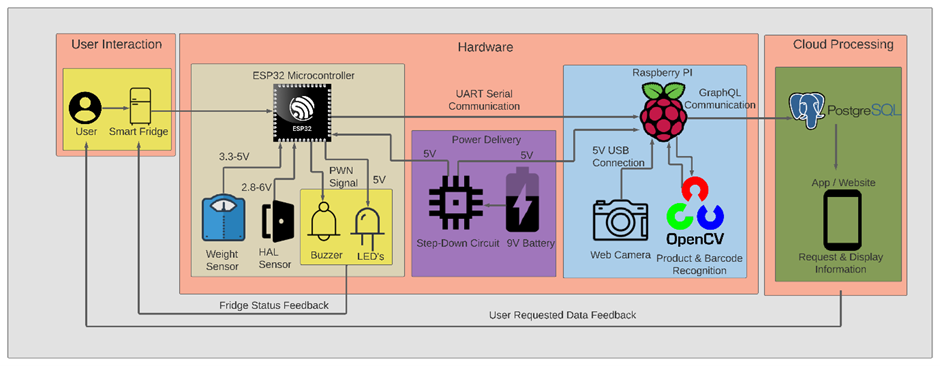
\includegraphics[width=1\textwidth]{Chapter 2/SystemOverview.png}
    \caption{System Overview Block Diagram}
    \label{fig:blockdia}
\end{figure} 

The project can be split into 3 main groups: the microprocessor group who will design the hardware which will collect the data, the Raspberry Pi group who will use OpenCV to detect the item and the cloud processing team who will deal with the server and website side of the design.
Within each group the tasks can be split between each member.
For example, in the microprocessor team, each member can be assigned to a different component and in the cloud processing team one member can focus on the front-end design and the other on the back end.
By splitting the project into smaller objectives, work can be completed independently and in parallel and the number dependencies between members can be reduced.
This will make the project run much more efficiently.
The individual teams will however need to communicate when planning on how to integrate the work together.
The sub systems and their dependencies have been outlined in table 'XXXXXXXXXXXXXX'.

\subsection{Dependency Table [IB]}
% Please add the following required packages to your document preamble:
% \usepackage{longtable}
% Note: It may be necessary to compile the document several times to get a multi-page table to line up properly
\small
\begin{longtable}[c]{|l|l|l|}
    \caption{Member Contributions and Goals}
    \label{tab:conrib}\\
    \hline
    Team Member &
      Contributions &
      Aims \\ \hline
    \endfirsthead
    %
    \endhead
    %
    Isaac Baglin - IB &
      \begin{tabular}[c]{@{}l@{}}Design Brief: Overview, SAGE assessment\\ form \\  \\ Project Work: Weight Sensor, Esp Camera\\ Module, Buzzer and Debugging  \\  \\ Final Report: System Overview, Smart\\ Fridge Dependency Table, Smart Fridge\\ MOSCOW Diagram, SWOT Analysis, Client\\ Brief Requirement Checklist, Phase Diagram\\ and Description, Weight Sensor Development,\\ Esp32-Wrover Dec-Board Camera\\ Development, Buzzer Development.\end{tabular} &
      \begin{tabular}[c]{@{}l@{}}My goal for this project was to develop\\ skills in systems engineering. To do this,\\ I put myself on the microprocessor team\\ so that I could plan, design, and integrate\\ subsystems.\end{tabular} \\ \hline
    \begin{tabular}[c]{@{}l@{}}Jamie \\ Gomez - JG\end{tabular} &
      \begin{tabular}[c]{@{}l@{}}Design Brief:  Project Management \\  \\ Project Work: Barcode detection, box design \\  \\ Final Report: Economic benefits, Barcode\\ detection, box design prototype 1\end{tabular} &
      \begin{tabular}[c]{@{}l@{}}My aim for this project was to develop my\\ teamwork skills. This was achieved mainly\\ when working on the box design where, \\ throughout the project, it was necessary\\ to listen to the requirements of each team\\ to design a box that best fitted everyone’s\\ needs. \\  \\ With barcode detection my aim was to find\\ and test suitable algorithms in order to\\ select the best one for this product.\end{tabular} \\ \hline
    \begin{tabular}[c]{@{}l@{}}Hamzah \\ Hasnain - HH\end{tabular} &
      \begin{tabular}[c]{@{}l@{}}Design Brief: Sustainability \\  \\ Project Work: Website Creation,\\ LEDs \\  \\ Final Report: Website, LEDs,\\ Sustainability, Circular Economy\end{tabular} &
      \begin{tabular}[c]{@{}l@{}}My goals for this project were to develop my\\ skills, specifically my skills in software and\\ programming. I took responsibility of creating\\ a website. Since I had not previously created\\ a website, there was a lot to learn. Learn how\\ web applications and hardware are integrated \\ I also wanted to gain experience with\\ programming hardware and understand\\ different methods of achieving a software-\\ hardware solution.\end{tabular} \\ \hline
    \begin{tabular}[c]{@{}l@{}}Ioanna \\ Papanikolaou - IP\end{tabular} &
      \begin{tabular}[c]{@{}l@{}}Design Brief: Technical Outline,Sustainability\\ discussion \\  \\ Project Work: \\ Object detection, character recognition,\\ model training  \\  \\ Final Report: Social, Economic and\\ Environmental impacts discussion, Software\\ Section\end{tabular} &
      \begin{tabular}[c]{@{}l@{}}My goals for this project were to develop my\\ software and team working skills. I was in the\\ software team with the aim of developing a \\ model that would classify the objects, acting\\ as an object recognition system. It was also\\ important for me to improve my teamwork\\ skills especially in software as so far I have\\ been mainly working on my own.\end{tabular} \\ \hline
    Yohan John - YJ &
      \begin{tabular}[c]{@{}l@{}}Design Brief: Technical Outline \\  \\ Project Work:  Architect the firmware code,\\ Hal Sensor Integration, Software – Timer\\ for buzzer feature. Comms between\\ raspberry pi and esp32, Debugging.\\ Designed Prototype 1. Designed and\\ built Prototype2 \\  \\ Final Report:  Hardware Outline, Firmware\\ Code, and Box Design and Build Prototyp2\end{tabular} &
      \begin{tabular}[c]{@{}l@{}}My goals for the group project included\\ developing my skills in both the technical\\ and management side. I wanted to take\\ more responsibility for organising the team\\ and architecting the software for the\\ microcontroller. I also aim to be an active\\ team member and contribute resources\\ when required.\end{tabular} \\ \hline
    \begin{tabular}[c]{@{}l@{}}Alexandre\\ Symeonidis-Herzig - ASH\end{tabular} &
      \begin{tabular}[c]{@{}l@{}}Design Brief: Appendices, Latex Compiling,\\ Revising document.  \\  \\ Project Work: Designed Pi Hat (PCB), Power\\ distribution board, Developed React Native\\ App and Created Supabase DB. \\  \\ Final Report: Tech background, Pi Hat PCB\\ design, Power distribution, Mobile App,\\ Supabase DB, Raspberry Pi Refactor\\ as well as compiling in LaTeX, editing\\ the document and formatting citations.\end{tabular} &
      \begin{tabular}[c]{@{}l@{}}To learn about and integrate all the \\ components for an app, from databases\\ and hosting to UI design and functionality.  \\   \\ Also, to focus on the learning the planning\\ required to get a more complicated project\\ from idea to prototype especially with a\\ larger team.\end{tabular} \\ \hline
    Alfie Walding - AW &
      \begin{tabular}[c]{@{}l@{}}Design Brief: Gantt Chart, Project\\ Management, Compiling and Revising\\ document.  \\  \\ Project Work: Raspberry Pi installation\\ and setup, Raspberry Pi camera setup,\\ Barcode detection development,\\ Raspberry Pi Serial communication,\\ Barcode detection integration, OCR code\\ integration, Product detection integration,\\ Supabase database integration and\\ Raspberry Pi refactoring. \\  \\ Final Report: Introduction, Pi Overview,\\ Pi camera, Pi serial input, Pi integration,\\ Pi refactoring as well as compiling and\\ revising the document.\end{tabular} &
      \begin{tabular}[c]{@{}l@{}}To successfully integrate and combine the \\ character, product, and barcode detection\\ code, onto the Raspberry Pi. The code should\\ function together flawlessly with compatibility\\ issues being fixed and required modules \\ imported. \\  \\ To receive data from the ESP and process it \\ into a format that can be communicated to \\ the database.  \\  \\ To successfully detect barcodes in images so\\ they can be sent to the database. \\  \\ To develop skills and knowledge of the\\ Raspberry Pi and the Linux operating system.\end{tabular} \\ \hline
\end{longtable}

\subsection{MOSCOW Diagram [IB]}
% Please add the following required packages to your document preamble:
% \usepackage{longtable}
% Note: It may be necessary to compile the document several times to get a multi-page table to line up properly
\small
\begin{longtable}[c]{|l|l|l|}
    \caption{Member Contributions and Goals}
    \label{tab:conrib}\\
    \hline
    Team Member &
      Contributions &
      Aims \\ \hline
    \endfirsthead
    %
    \endhead
    %
    Isaac Baglin - IB &
      \begin{tabular}[c]{@{}l@{}}Design Brief: Overview, SAGE assessment\\ form \\  \\ Project Work: Weight Sensor, Esp Camera\\ Module, Buzzer and Debugging  \\  \\ Final Report: System Overview, Smart\\ Fridge Dependency Table, Smart Fridge\\ MOSCOW Diagram, SWOT Analysis, Client\\ Brief Requirement Checklist, Phase Diagram\\ and Description, Weight Sensor Development,\\ Esp32-Wrover Dec-Board Camera\\ Development, Buzzer Development.\end{tabular} &
      \begin{tabular}[c]{@{}l@{}}My goal for this project was to develop\\ skills in systems engineering. To do this,\\ I put myself on the microprocessor team\\ so that I could plan, design, and integrate\\ subsystems.\end{tabular} \\ \hline
    \begin{tabular}[c]{@{}l@{}}Jamie \\ Gomez - JG\end{tabular} &
      \begin{tabular}[c]{@{}l@{}}Design Brief:  Project Management \\  \\ Project Work: Barcode detection, box design \\  \\ Final Report: Economic benefits, Barcode\\ detection, box design prototype 1\end{tabular} &
      \begin{tabular}[c]{@{}l@{}}My aim for this project was to develop my\\ teamwork skills. This was achieved mainly\\ when working on the box design where, \\ throughout the project, it was necessary\\ to listen to the requirements of each team\\ to design a box that best fitted everyone’s\\ needs. \\  \\ With barcode detection my aim was to find\\ and test suitable algorithms in order to\\ select the best one for this product.\end{tabular} \\ \hline
    \begin{tabular}[c]{@{}l@{}}Hamzah \\ Hasnain - HH\end{tabular} &
      \begin{tabular}[c]{@{}l@{}}Design Brief: Sustainability \\  \\ Project Work: Website Creation,\\ LEDs \\  \\ Final Report: Website, LEDs,\\ Sustainability, Circular Economy\end{tabular} &
      \begin{tabular}[c]{@{}l@{}}My goals for this project were to develop my\\ skills, specifically my skills in software and\\ programming. I took responsibility of creating\\ a website. Since I had not previously created\\ a website, there was a lot to learn. Learn how\\ web applications and hardware are integrated \\ I also wanted to gain experience with\\ programming hardware and understand\\ different methods of achieving a software-\\ hardware solution.\end{tabular} \\ \hline
    \begin{tabular}[c]{@{}l@{}}Ioanna \\ Papanikolaou - IP\end{tabular} &
      \begin{tabular}[c]{@{}l@{}}Design Brief: Technical Outline,Sustainability\\ discussion \\  \\ Project Work: \\ Object detection, character recognition,\\ model training  \\  \\ Final Report: Social, Economic and\\ Environmental impacts discussion, Software\\ Section\end{tabular} &
      \begin{tabular}[c]{@{}l@{}}My goals for this project were to develop my\\ software and team working skills. I was in the\\ software team with the aim of developing a \\ model that would classify the objects, acting\\ as an object recognition system. It was also\\ important for me to improve my teamwork\\ skills especially in software as so far I have\\ been mainly working on my own.\end{tabular} \\ \hline
    Yohan John - YJ &
      \begin{tabular}[c]{@{}l@{}}Design Brief: Technical Outline \\  \\ Project Work:  Architect the firmware code,\\ Hal Sensor Integration, Software – Timer\\ for buzzer feature. Comms between\\ raspberry pi and esp32, Debugging.\\ Designed Prototype 1. Designed and\\ built Prototype2 \\  \\ Final Report:  Hardware Outline, Firmware\\ Code, and Box Design and Build Prototyp2\end{tabular} &
      \begin{tabular}[c]{@{}l@{}}My goals for the group project included\\ developing my skills in both the technical\\ and management side. I wanted to take\\ more responsibility for organising the team\\ and architecting the software for the\\ microcontroller. I also aim to be an active\\ team member and contribute resources\\ when required.\end{tabular} \\ \hline
    \begin{tabular}[c]{@{}l@{}}Alexandre\\ Symeonidis-Herzig - ASH\end{tabular} &
      \begin{tabular}[c]{@{}l@{}}Design Brief: Appendices, Latex Compiling,\\ Revising document.  \\  \\ Project Work: Designed Pi Hat (PCB), Power\\ distribution board, Developed React Native\\ App and Created Supabase DB. \\  \\ Final Report: Tech background, Pi Hat PCB\\ design, Power distribution, Mobile App,\\ Supabase DB, Raspberry Pi Refactor\\ as well as compiling in LaTeX, editing\\ the document and formatting citations.\end{tabular} &
      \begin{tabular}[c]{@{}l@{}}To learn about and integrate all the \\ components for an app, from databases\\ and hosting to UI design and functionality.  \\   \\ Also, to focus on the learning the planning\\ required to get a more complicated project\\ from idea to prototype especially with a\\ larger team.\end{tabular} \\ \hline
    Alfie Walding - AW &
      \begin{tabular}[c]{@{}l@{}}Design Brief: Gantt Chart, Project\\ Management, Compiling and Revising\\ document.  \\  \\ Project Work: Raspberry Pi installation\\ and setup, Raspberry Pi camera setup,\\ Barcode detection development,\\ Raspberry Pi Serial communication,\\ Barcode detection integration, OCR code\\ integration, Product detection integration,\\ Supabase database integration and\\ Raspberry Pi refactoring. \\  \\ Final Report: Introduction, Pi Overview,\\ Pi camera, Pi serial input, Pi integration,\\ Pi refactoring as well as compiling and\\ revising the document.\end{tabular} &
      \begin{tabular}[c]{@{}l@{}}To successfully integrate and combine the \\ character, product, and barcode detection\\ code, onto the Raspberry Pi. The code should\\ function together flawlessly with compatibility\\ issues being fixed and required modules \\ imported. \\  \\ To receive data from the ESP and process it \\ into a format that can be communicated to \\ the database.  \\  \\ To successfully detect barcodes in images so\\ they can be sent to the database. \\  \\ To develop skills and knowledge of the\\ Raspberry Pi and the Linux operating system.\end{tabular} \\ \hline
\end{longtable}

\subsection{SWOT Analysis [IB]}
% Please add the following required packages to your document preamble:
% \usepackage{longtable}
% Note: It may be necessary to compile the document several times to get a multi-page table to line up properly
\small
\begin{longtable}[c]{|l|l|l|}
    \caption{Member Contributions and Goals}
    \label{tab:conrib}\\
    \hline
    Team Member &
      Contributions &
      Aims \\ \hline
    \endfirsthead
    %
    \endhead
    %
    Isaac Baglin - IB &
      \begin{tabular}[c]{@{}l@{}}Design Brief: Overview, SAGE assessment\\ form \\  \\ Project Work: Weight Sensor, Esp Camera\\ Module, Buzzer and Debugging  \\  \\ Final Report: System Overview, Smart\\ Fridge Dependency Table, Smart Fridge\\ MOSCOW Diagram, SWOT Analysis, Client\\ Brief Requirement Checklist, Phase Diagram\\ and Description, Weight Sensor Development,\\ Esp32-Wrover Dec-Board Camera\\ Development, Buzzer Development.\end{tabular} &
      \begin{tabular}[c]{@{}l@{}}My goal for this project was to develop\\ skills in systems engineering. To do this,\\ I put myself on the microprocessor team\\ so that I could plan, design, and integrate\\ subsystems.\end{tabular} \\ \hline
    \begin{tabular}[c]{@{}l@{}}Jamie \\ Gomez - JG\end{tabular} &
      \begin{tabular}[c]{@{}l@{}}Design Brief:  Project Management \\  \\ Project Work: Barcode detection, box design \\  \\ Final Report: Economic benefits, Barcode\\ detection, box design prototype 1\end{tabular} &
      \begin{tabular}[c]{@{}l@{}}My aim for this project was to develop my\\ teamwork skills. This was achieved mainly\\ when working on the box design where, \\ throughout the project, it was necessary\\ to listen to the requirements of each team\\ to design a box that best fitted everyone’s\\ needs. \\  \\ With barcode detection my aim was to find\\ and test suitable algorithms in order to\\ select the best one for this product.\end{tabular} \\ \hline
    \begin{tabular}[c]{@{}l@{}}Hamzah \\ Hasnain - HH\end{tabular} &
      \begin{tabular}[c]{@{}l@{}}Design Brief: Sustainability \\  \\ Project Work: Website Creation,\\ LEDs \\  \\ Final Report: Website, LEDs,\\ Sustainability, Circular Economy\end{tabular} &
      \begin{tabular}[c]{@{}l@{}}My goals for this project were to develop my\\ skills, specifically my skills in software and\\ programming. I took responsibility of creating\\ a website. Since I had not previously created\\ a website, there was a lot to learn. Learn how\\ web applications and hardware are integrated \\ I also wanted to gain experience with\\ programming hardware and understand\\ different methods of achieving a software-\\ hardware solution.\end{tabular} \\ \hline
    \begin{tabular}[c]{@{}l@{}}Ioanna \\ Papanikolaou - IP\end{tabular} &
      \begin{tabular}[c]{@{}l@{}}Design Brief: Technical Outline,Sustainability\\ discussion \\  \\ Project Work: \\ Object detection, character recognition,\\ model training  \\  \\ Final Report: Social, Economic and\\ Environmental impacts discussion, Software\\ Section\end{tabular} &
      \begin{tabular}[c]{@{}l@{}}My goals for this project were to develop my\\ software and team working skills. I was in the\\ software team with the aim of developing a \\ model that would classify the objects, acting\\ as an object recognition system. It was also\\ important for me to improve my teamwork\\ skills especially in software as so far I have\\ been mainly working on my own.\end{tabular} \\ \hline
    Yohan John - YJ &
      \begin{tabular}[c]{@{}l@{}}Design Brief: Technical Outline \\  \\ Project Work:  Architect the firmware code,\\ Hal Sensor Integration, Software – Timer\\ for buzzer feature. Comms between\\ raspberry pi and esp32, Debugging.\\ Designed Prototype 1. Designed and\\ built Prototype2 \\  \\ Final Report:  Hardware Outline, Firmware\\ Code, and Box Design and Build Prototyp2\end{tabular} &
      \begin{tabular}[c]{@{}l@{}}My goals for the group project included\\ developing my skills in both the technical\\ and management side. I wanted to take\\ more responsibility for organising the team\\ and architecting the software for the\\ microcontroller. I also aim to be an active\\ team member and contribute resources\\ when required.\end{tabular} \\ \hline
    \begin{tabular}[c]{@{}l@{}}Alexandre\\ Symeonidis-Herzig - ASH\end{tabular} &
      \begin{tabular}[c]{@{}l@{}}Design Brief: Appendices, Latex Compiling,\\ Revising document.  \\  \\ Project Work: Designed Pi Hat (PCB), Power\\ distribution board, Developed React Native\\ App and Created Supabase DB. \\  \\ Final Report: Tech background, Pi Hat PCB\\ design, Power distribution, Mobile App,\\ Supabase DB, Raspberry Pi Refactor\\ as well as compiling in LaTeX, editing\\ the document and formatting citations.\end{tabular} &
      \begin{tabular}[c]{@{}l@{}}To learn about and integrate all the \\ components for an app, from databases\\ and hosting to UI design and functionality.  \\   \\ Also, to focus on the learning the planning\\ required to get a more complicated project\\ from idea to prototype especially with a\\ larger team.\end{tabular} \\ \hline
    Alfie Walding - AW &
      \begin{tabular}[c]{@{}l@{}}Design Brief: Gantt Chart, Project\\ Management, Compiling and Revising\\ document.  \\  \\ Project Work: Raspberry Pi installation\\ and setup, Raspberry Pi camera setup,\\ Barcode detection development,\\ Raspberry Pi Serial communication,\\ Barcode detection integration, OCR code\\ integration, Product detection integration,\\ Supabase database integration and\\ Raspberry Pi refactoring. \\  \\ Final Report: Introduction, Pi Overview,\\ Pi camera, Pi serial input, Pi integration,\\ Pi refactoring as well as compiling and\\ revising the document.\end{tabular} &
      \begin{tabular}[c]{@{}l@{}}To successfully integrate and combine the \\ character, product, and barcode detection\\ code, onto the Raspberry Pi. The code should\\ function together flawlessly with compatibility\\ issues being fixed and required modules \\ imported. \\  \\ To receive data from the ESP and process it \\ into a format that can be communicated to \\ the database.  \\  \\ To successfully detect barcodes in images so\\ they can be sent to the database. \\  \\ To develop skills and knowledge of the\\ Raspberry Pi and the Linux operating system.\end{tabular} \\ \hline
\end{longtable}

\subsection{Client Requirements [IB]}
% Please add the following required packages to your document preamble:
% \usepackage{longtable}
% Note: It may be necessary to compile the document several times to get a multi-page table to line up properly
\small
\begin{longtable}[c]{|l|l|l|}
    \caption{Member Contributions and Goals}
    \label{tab:conrib}\\
    \hline
    Team Member &
      Contributions &
      Aims \\ \hline
    \endfirsthead
    %
    \endhead
    %
    Isaac Baglin - IB &
      \begin{tabular}[c]{@{}l@{}}Design Brief: Overview, SAGE assessment\\ form \\  \\ Project Work: Weight Sensor, Esp Camera\\ Module, Buzzer and Debugging  \\  \\ Final Report: System Overview, Smart\\ Fridge Dependency Table, Smart Fridge\\ MOSCOW Diagram, SWOT Analysis, Client\\ Brief Requirement Checklist, Phase Diagram\\ and Description, Weight Sensor Development,\\ Esp32-Wrover Dec-Board Camera\\ Development, Buzzer Development.\end{tabular} &
      \begin{tabular}[c]{@{}l@{}}My goal for this project was to develop\\ skills in systems engineering. To do this,\\ I put myself on the microprocessor team\\ so that I could plan, design, and integrate\\ subsystems.\end{tabular} \\ \hline
    \begin{tabular}[c]{@{}l@{}}Jamie \\ Gomez - JG\end{tabular} &
      \begin{tabular}[c]{@{}l@{}}Design Brief:  Project Management \\  \\ Project Work: Barcode detection, box design \\  \\ Final Report: Economic benefits, Barcode\\ detection, box design prototype 1\end{tabular} &
      \begin{tabular}[c]{@{}l@{}}My aim for this project was to develop my\\ teamwork skills. This was achieved mainly\\ when working on the box design where, \\ throughout the project, it was necessary\\ to listen to the requirements of each team\\ to design a box that best fitted everyone’s\\ needs. \\  \\ With barcode detection my aim was to find\\ and test suitable algorithms in order to\\ select the best one for this product.\end{tabular} \\ \hline
    \begin{tabular}[c]{@{}l@{}}Hamzah \\ Hasnain - HH\end{tabular} &
      \begin{tabular}[c]{@{}l@{}}Design Brief: Sustainability \\  \\ Project Work: Website Creation,\\ LEDs \\  \\ Final Report: Website, LEDs,\\ Sustainability, Circular Economy\end{tabular} &
      \begin{tabular}[c]{@{}l@{}}My goals for this project were to develop my\\ skills, specifically my skills in software and\\ programming. I took responsibility of creating\\ a website. Since I had not previously created\\ a website, there was a lot to learn. Learn how\\ web applications and hardware are integrated \\ I also wanted to gain experience with\\ programming hardware and understand\\ different methods of achieving a software-\\ hardware solution.\end{tabular} \\ \hline
    \begin{tabular}[c]{@{}l@{}}Ioanna \\ Papanikolaou - IP\end{tabular} &
      \begin{tabular}[c]{@{}l@{}}Design Brief: Technical Outline,Sustainability\\ discussion \\  \\ Project Work: \\ Object detection, character recognition,\\ model training  \\  \\ Final Report: Social, Economic and\\ Environmental impacts discussion, Software\\ Section\end{tabular} &
      \begin{tabular}[c]{@{}l@{}}My goals for this project were to develop my\\ software and team working skills. I was in the\\ software team with the aim of developing a \\ model that would classify the objects, acting\\ as an object recognition system. It was also\\ important for me to improve my teamwork\\ skills especially in software as so far I have\\ been mainly working on my own.\end{tabular} \\ \hline
    Yohan John - YJ &
      \begin{tabular}[c]{@{}l@{}}Design Brief: Technical Outline \\  \\ Project Work:  Architect the firmware code,\\ Hal Sensor Integration, Software – Timer\\ for buzzer feature. Comms between\\ raspberry pi and esp32, Debugging.\\ Designed Prototype 1. Designed and\\ built Prototype2 \\  \\ Final Report:  Hardware Outline, Firmware\\ Code, and Box Design and Build Prototyp2\end{tabular} &
      \begin{tabular}[c]{@{}l@{}}My goals for the group project included\\ developing my skills in both the technical\\ and management side. I wanted to take\\ more responsibility for organising the team\\ and architecting the software for the\\ microcontroller. I also aim to be an active\\ team member and contribute resources\\ when required.\end{tabular} \\ \hline
    \begin{tabular}[c]{@{}l@{}}Alexandre\\ Symeonidis-Herzig - ASH\end{tabular} &
      \begin{tabular}[c]{@{}l@{}}Design Brief: Appendices, Latex Compiling,\\ Revising document.  \\  \\ Project Work: Designed Pi Hat (PCB), Power\\ distribution board, Developed React Native\\ App and Created Supabase DB. \\  \\ Final Report: Tech background, Pi Hat PCB\\ design, Power distribution, Mobile App,\\ Supabase DB, Raspberry Pi Refactor\\ as well as compiling in LaTeX, editing\\ the document and formatting citations.\end{tabular} &
      \begin{tabular}[c]{@{}l@{}}To learn about and integrate all the \\ components for an app, from databases\\ and hosting to UI design and functionality.  \\   \\ Also, to focus on the learning the planning\\ required to get a more complicated project\\ from idea to prototype especially with a\\ larger team.\end{tabular} \\ \hline
    Alfie Walding - AW &
      \begin{tabular}[c]{@{}l@{}}Design Brief: Gantt Chart, Project\\ Management, Compiling and Revising\\ document.  \\  \\ Project Work: Raspberry Pi installation\\ and setup, Raspberry Pi camera setup,\\ Barcode detection development,\\ Raspberry Pi Serial communication,\\ Barcode detection integration, OCR code\\ integration, Product detection integration,\\ Supabase database integration and\\ Raspberry Pi refactoring. \\  \\ Final Report: Introduction, Pi Overview,\\ Pi camera, Pi serial input, Pi integration,\\ Pi refactoring as well as compiling and\\ revising the document.\end{tabular} &
      \begin{tabular}[c]{@{}l@{}}To successfully integrate and combine the \\ character, product, and barcode detection\\ code, onto the Raspberry Pi. The code should\\ function together flawlessly with compatibility\\ issues being fixed and required modules \\ imported. \\  \\ To receive data from the ESP and process it \\ into a format that can be communicated to \\ the database.  \\  \\ To successfully detect barcodes in images so\\ they can be sent to the database. \\  \\ To develop skills and knowledge of the\\ Raspberry Pi and the Linux operating system.\end{tabular} \\ \hline
\end{longtable}

\subsection{Phase Diagram [IB]}

\begin{figure}[H]        
    \centering
    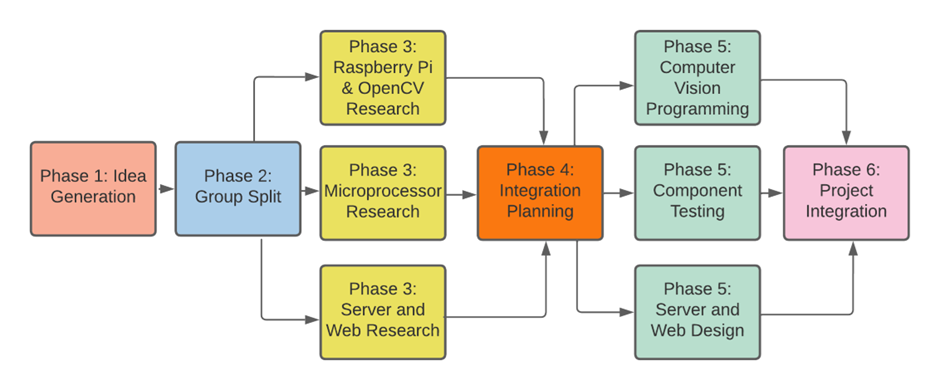
\includegraphics[width=1\textwidth]{Chapter 2/PhaseDiagram.png}
    \caption{Phase Diagram}
    \label{fig:phasediag}
\end{figure} 

The first phase of the project was to generate ideas for the project which followed the specification and vote on which idea to put forward.
Phase 2 is when the group discusses the individual members strengths and weaknesses and decides who is best suited to each team.
Phase 3 is the research phase, and it involves looking into what software and components could be used whilst considering their feasibility.

At the end of this phase a plan should be formed to start designing and testing the tasks of each group as well as ordering the required parts.
Phase 4 is aimed at coming together as a group and forming a plan to integrate the individual teams work together.
This includes discussions of dependencies that each sub team have on each other.
Phase 5 is when the individual teams build and test their work and phase 6 is when the work of the 3 teams is integrated together.

\section{Hardware}
\subsection{Hardware Overview}

Hardware aims to work with the software to help the user track what is in the fridge and how long the door is kept open.
The weight sensor tracks the direction of the object in and out of the Smart-Fridge.
The Hal Switch is aware of when the door is open and closed.
The tasks mentioned before run on the ESP-32 microcontroller by Espressif.


This section will also discuss how each of these works in detail, with a record of their power distribution.


\subsection{Power Distribution [ASH]}

The Smart Fridge consists of microcontrollers, logic boards and various sensors which all need to be powered at the appropriate voltage and possible current draw.
Below is a table with all power requirements.


% Please add the following required packages to your document preamble:
% \usepackage{longtable}
% Note: It may be necessary to compile the document several times to get a multi-page table to line up properly
\small
\begin{longtable}[c]{|l|l|l|}
    \caption{Member Contributions and Goals}
    \label{tab:conrib}\\
    \hline
    Team Member &
      Contributions &
      Aims \\ \hline
    \endfirsthead
    %
    \endhead
    %
    Isaac Baglin - IB &
      \begin{tabular}[c]{@{}l@{}}Design Brief: Overview, SAGE assessment\\ form \\  \\ Project Work: Weight Sensor, Esp Camera\\ Module, Buzzer and Debugging  \\  \\ Final Report: System Overview, Smart\\ Fridge Dependency Table, Smart Fridge\\ MOSCOW Diagram, SWOT Analysis, Client\\ Brief Requirement Checklist, Phase Diagram\\ and Description, Weight Sensor Development,\\ Esp32-Wrover Dec-Board Camera\\ Development, Buzzer Development.\end{tabular} &
      \begin{tabular}[c]{@{}l@{}}My goal for this project was to develop\\ skills in systems engineering. To do this,\\ I put myself on the microprocessor team\\ so that I could plan, design, and integrate\\ subsystems.\end{tabular} \\ \hline
    \begin{tabular}[c]{@{}l@{}}Jamie \\ Gomez - JG\end{tabular} &
      \begin{tabular}[c]{@{}l@{}}Design Brief:  Project Management \\  \\ Project Work: Barcode detection, box design \\  \\ Final Report: Economic benefits, Barcode\\ detection, box design prototype 1\end{tabular} &
      \begin{tabular}[c]{@{}l@{}}My aim for this project was to develop my\\ teamwork skills. This was achieved mainly\\ when working on the box design where, \\ throughout the project, it was necessary\\ to listen to the requirements of each team\\ to design a box that best fitted everyone’s\\ needs. \\  \\ With barcode detection my aim was to find\\ and test suitable algorithms in order to\\ select the best one for this product.\end{tabular} \\ \hline
    \begin{tabular}[c]{@{}l@{}}Hamzah \\ Hasnain - HH\end{tabular} &
      \begin{tabular}[c]{@{}l@{}}Design Brief: Sustainability \\  \\ Project Work: Website Creation,\\ LEDs \\  \\ Final Report: Website, LEDs,\\ Sustainability, Circular Economy\end{tabular} &
      \begin{tabular}[c]{@{}l@{}}My goals for this project were to develop my\\ skills, specifically my skills in software and\\ programming. I took responsibility of creating\\ a website. Since I had not previously created\\ a website, there was a lot to learn. Learn how\\ web applications and hardware are integrated \\ I also wanted to gain experience with\\ programming hardware and understand\\ different methods of achieving a software-\\ hardware solution.\end{tabular} \\ \hline
    \begin{tabular}[c]{@{}l@{}}Ioanna \\ Papanikolaou - IP\end{tabular} &
      \begin{tabular}[c]{@{}l@{}}Design Brief: Technical Outline,Sustainability\\ discussion \\  \\ Project Work: \\ Object detection, character recognition,\\ model training  \\  \\ Final Report: Social, Economic and\\ Environmental impacts discussion, Software\\ Section\end{tabular} &
      \begin{tabular}[c]{@{}l@{}}My goals for this project were to develop my\\ software and team working skills. I was in the\\ software team with the aim of developing a \\ model that would classify the objects, acting\\ as an object recognition system. It was also\\ important for me to improve my teamwork\\ skills especially in software as so far I have\\ been mainly working on my own.\end{tabular} \\ \hline
    Yohan John - YJ &
      \begin{tabular}[c]{@{}l@{}}Design Brief: Technical Outline \\  \\ Project Work:  Architect the firmware code,\\ Hal Sensor Integration, Software – Timer\\ for buzzer feature. Comms between\\ raspberry pi and esp32, Debugging.\\ Designed Prototype 1. Designed and\\ built Prototype2 \\  \\ Final Report:  Hardware Outline, Firmware\\ Code, and Box Design and Build Prototyp2\end{tabular} &
      \begin{tabular}[c]{@{}l@{}}My goals for the group project included\\ developing my skills in both the technical\\ and management side. I wanted to take\\ more responsibility for organising the team\\ and architecting the software for the\\ microcontroller. I also aim to be an active\\ team member and contribute resources\\ when required.\end{tabular} \\ \hline
    \begin{tabular}[c]{@{}l@{}}Alexandre\\ Symeonidis-Herzig - ASH\end{tabular} &
      \begin{tabular}[c]{@{}l@{}}Design Brief: Appendices, Latex Compiling,\\ Revising document.  \\  \\ Project Work: Designed Pi Hat (PCB), Power\\ distribution board, Developed React Native\\ App and Created Supabase DB. \\  \\ Final Report: Tech background, Pi Hat PCB\\ design, Power distribution, Mobile App,\\ Supabase DB, Raspberry Pi Refactor\\ as well as compiling in LaTeX, editing\\ the document and formatting citations.\end{tabular} &
      \begin{tabular}[c]{@{}l@{}}To learn about and integrate all the \\ components for an app, from databases\\ and hosting to UI design and functionality.  \\   \\ Also, to focus on the learning the planning\\ required to get a more complicated project\\ from idea to prototype especially with a\\ larger team.\end{tabular} \\ \hline
    Alfie Walding - AW &
      \begin{tabular}[c]{@{}l@{}}Design Brief: Gantt Chart, Project\\ Management, Compiling and Revising\\ document.  \\  \\ Project Work: Raspberry Pi installation\\ and setup, Raspberry Pi camera setup,\\ Barcode detection development,\\ Raspberry Pi Serial communication,\\ Barcode detection integration, OCR code\\ integration, Product detection integration,\\ Supabase database integration and\\ Raspberry Pi refactoring. \\  \\ Final Report: Introduction, Pi Overview,\\ Pi camera, Pi serial input, Pi integration,\\ Pi refactoring as well as compiling and\\ revising the document.\end{tabular} &
      \begin{tabular}[c]{@{}l@{}}To successfully integrate and combine the \\ character, product, and barcode detection\\ code, onto the Raspberry Pi. The code should\\ function together flawlessly with compatibility\\ issues being fixed and required modules \\ imported. \\  \\ To receive data from the ESP and process it \\ into a format that can be communicated to \\ the database.  \\  \\ To successfully detect barcodes in images so\\ they can be sent to the database. \\  \\ To develop skills and knowledge of the\\ Raspberry Pi and the Linux operating system.\end{tabular} \\ \hline
\end{longtable}

As can be seen on the table above, the RPI and ESP-32 consume most of the power and the total system power draw will be around 17W.
However, we will require two separate voltage rails to power the various components, one at 5V and one at 3.3V.
The initial plan to achieve this was to use the adjustable variants of the LM2596.
Using these we could output voltages in the range of 1.2V to 37V at up to 3A with a typical efficiency of 73% [TI DATA SHEET].
We could then power the Smart Fridge's logic components using a 9V power supply which will feed into the two power regulators.
The schematic for these power supplies can be seen below in Figure [X].
Only one power supply is shown in the schematic, as we would use variable resistors to fine-tune the exact voltage in this prototype.


Our 3.3V power supply would be used to power the ESP-32, which has a maximum power draw of 1.65W meaning we will need to input 2.26W (as 2.26* 73% = 1.65W).
At our input voltage of 9V, we would need a minimum current of 0.25A.
Our 5V power supply would be used to power the remaining components, primarily the Raspberry Pi 3B+.
This has a maximum power draw of 15.0525W or roughly 15W.
Meaning we would need to input 22.55W (as 22.55* 73% = 15W) to the power regulator.
At 9V this means we would need an input current of at least 2.28A.
This means for both our power supplies we would need to provide 2.53A at 9V.
To add a safety margin (and due to power supply availability) we would use a 9V power supply capable of providing up the 3A.



Unfortunately, this initial design was not able to be realized due to LM2596 being unavailable.
Availability of this component was not checked before PCB was designed and ordered; this flaw is further discussed in the PCB section.
Fortunately powering the device via other means was also possible, as both the RPI and ESP32 boards have power regulation built in.
This means we can power the RPI using its Micro USB port and power supply capable of delivering the desired 2.5A and then use the GPIO pins 5V output to power the ESP32.
The ESP32 will create a 3.3V output using its built-in power regulator.
The other components listed in table [] above can then be powered using the logic boards outputs and the webcam will still be powered by the RPI as would have been the case originally.



This method is simpler than our previously proposed solution, however there are two major drawbacks; lower efficiency and lower overall power.
Our initial plan used switch-mode power supplies, which adjusts voltage using high-frequencies switching to achieve a high efficiency, however using the onboard voltage regulator of the RPI will give us much lower efficiencies, ranging from 30% to 60%, as they function as variable resistors and turn excess voltage into heat.
These lower efficiencies pose a few problems, first is that the device will draw more power as all times which goes against sustainability targets and may lower a product's energy efficiency rating.
Furthermore, the extra heat may damage the esp32 board, though this is unlikely at our power range, and may cause the RPI to throttle its clock-speed to prevent it from overheating, reducing performance which may be critical for computer vision tasks.
The other drawback is that the total available power to our system, even before inefficiencies, is reduced from 27W to 15W.
This is still enough power for all our systems, as table [] above lists the maximum desired currents, and the minimum power is much lower.
Reduced overall power could lead to power becoming intermittent especially to the webcam and ESP which are downstream from the PI.
However, the RPI documentation states that this should not be an issue as it can pass through around 5W to its GPIO and USB devices, and in practice we found this to hold true however the lack of margin is undesirable.


Overall, the power management did not go as planned due to, in part, the ongoing semiconductor shortage as well as poor planning on the component acquisition side.
However, we were able to pivot to provide a suitable solution and, given more time to order components or redesigning to use a different IC, could make use of the research that went into the original design.


\subsection{PI HAT [ASH]}

In order to securely connect and hold together the various components that make up the Smart Fridge, we designed a printed circuit board.
Using a PCB reduces the chance of connections coming loose, makes the design more compact and increases sturdiness.
In the case of the Smart Fridge, many of our components already come with their own boards (such as the ESP32 dev board or the RPI board) which is why our PCB is designed is designed more as a “motherboard” to hold and connect all the boards.
As the RPI is the largest component of the Smart Fridge the board will be designed as a RPI “Hat” (Hardware Attached on Top) which is a header board specification designed by the Raspberry Pi foundation [RPI GITHUB].
The specifications primairly consist of mechanical specifications, about size, rounding and screw-holes in the PCB, requirements for the 40-pin header used to attach to the RPI, and inclusion of an EEPROM (read only memory) with data about the HAT.
By following these specifications, we ensure that the PCB will fit atop the Raspberry PI and be recognized as HAT.
Our goals for this PCB were to create a board that can, compactly, fit together our various board and sensors, provide them with power and meet the RPI HAT specification.



The PCB was designed in KiCAD which is an open-source and free EDA (Electronic Design Automation) software suite.
KiCAD was chosen as I had previous experience in the software as well as the desire to ensure that anyone on the team be able to open, read and even edit the files using any computer as the software is readily available.
Furthermore KiCAD has a template for RPI HATs that ensure we achieve the desired specifications.
The first step involved placing all of the required components, which consisted mostly of components for the power distribution and connectors for the ESP and other sensors.
Then the appropriate connections where made, as provided by the Hardware team and the power distribution schematics.
A full schematics diagram can be seen on in the appendix [list section].
After this schematic was created the components all had to be given appropriate footprints and then placed on a board.
This completed design can be seen below in Figure [X].



This PCB was then ordered from JLBPCB and assembly began almost immediately of the available components.
Unfortunately there where some problems, firstly, as mentioned in the Power Distribution section the LM2596 were unavailable in our time frame meaning the full board could not be assembled.
Another problem came with the ESP32, as the exact model we ended up using was not the one communicated during the design of PCB and features different pin spacing than most ESP32s, meaning it was too wide to fit on the board.
Initially a “converter” board was considered to allow our new ESP to fit on the PCB, however due to the other problem a different solution was used.
The PCB was also larger than expected due to an export error when sending the files to the manufacturer.
These issues all compounded to leave us with a design that was not fit for function and was therefor abandoned for another solution, the progress up until this point can be seen in the picture below in figure [X].
The created files for the PCB could however easily be updated for a second version had time allowed.



Instead of the PCB, a perfboard was used.
This board was designed using the schematics created for the PCB, as all the connection remained relevant however the EEPROM and Power Distribution section where omitted due to time constraints and redesign respectively.
This board kept the form factor of being mounted atop the RPI, but due to the dropped EEPROM and dimension change can not be considered a PI HAT.
This solution however still serves the original purpose, and manged to provide much of the desired sturdiness and compactness of the original PCB design.


\subsection{Weight Sensor [IB]}

As mentioned previously, the purpose of the weight sensor is to determine whether an item is being placed into the fridge or taken out.
This can be determined if the weight increases, an item is being added and if the weight decreases, an item must be being removed.
The change in weight value will be assigned a direction variable which is communicated to the pi in order to remove or add an item.
For this process to work, the weight value doesn't need to be accurate, however, it must increase or decrease with a change in weight.

The weight sensor which will be used is the HX711 Load Cell.
A load cell contains strain gauges which convert tension on a beam into an electrical signal.
The HX711 contains an 8cm load cell with the strain gauges already attached.
There is also a A/D convertor to convert the tension signal into a usable digital signal for the esp32 to process.
The HX711 Load Cell was chosen specifically because it has libraries available on the Arduino IDE and is compatible with the Esp-32 board.
Figure 1 shows how the Load Cell, A/D convertor and Esp-32 are connected.

\begin{figure}[H]        
    \centering
    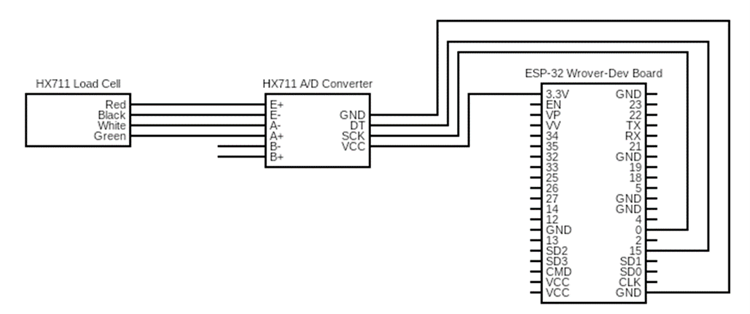
\includegraphics[width=1\textwidth]{Chapter 3/Weight Sensor/LoadCellCircuitDiagram.png}
    \caption{Load Cell Circuit Diagram}
    \label{fig:lccircuit}
\end{figure} 

On the load cell there are 4 holes, 2 on either side which allow us to secure a custom-made platform above and below the load cell.
Because the screws are off cantered, the load cell will be strained when an item is placed on it.
Our load cell is said to support up to 10kg.

\begin{figure}[H]        
    \centering
    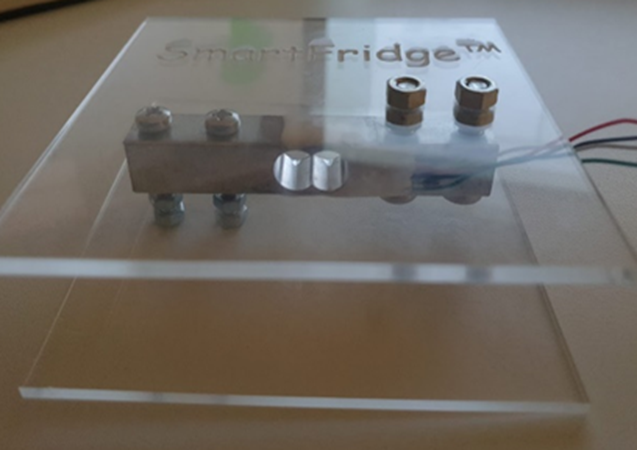
\includegraphics[width=1\textwidth]{Chapter 3/Weight Sensor/WeightSensorPicture.png}
    \caption{Load Cell Prototype}
    \label{fig:lcproto}
\end{figure} 

The HX711 load cell has an Arduino library which contains the necessary functions to calculate the mass in Kg.
Within the setup function, values for calibration\_factor and currentOffset are set.
These helps calibrate the weight to a reasonable value.
Within the loop the function get\_units is used to calculate the mass using the current currentOffset and calibration\_factor values.

\begin{figure}[H]        
    \centering
    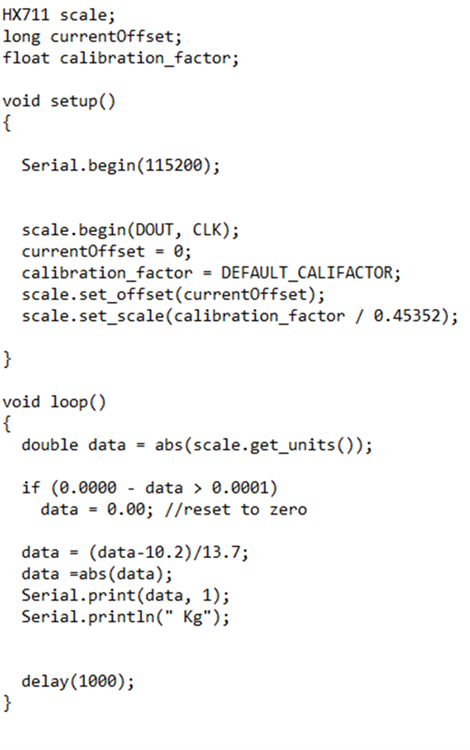
\includegraphics[width=.5\textwidth]{Chapter 3/Weight Sensor/WeightSensorCalibrationCode.png}
    \caption{Load Cell Calibration Code}
    \label{fig:lccode}
\end{figure} 

Often when nothing is placed on the load cell a negative mass is displayed due to an upward force from the table acting in opposition to the weight of the load cell.
To avoid this the mass will be set to zero if it goes negative.
Some manual calibrations are required to offset the fact that the weight can be affected by the weight of the platform as well as how tight the screws are.
Once the load cell has been fitted within the smart fridge these offset values will remain constant after resets.

During the earlier weeks of the project, the load cell platform hadn't been created yet and to test the load cell, it was balanced on a pair of books.
This meant that the strain gauge wasn't being strained correctly as the items were being placed directly on top of it rather than on the correct platform.
This meant that the values were incorrect and couldn't be calibrated correctly.
This resulted in many hours being wasted trying to figure out if something wasn't connected properly or trying to produce elaborate Arduino functions to automatically calibrate the load cell upon the program initializing.

Once a test platform was produced in week 7 using scrap pieces of acrylic, the load cell was able to be calibrated correctly and output accurate results.
An issue which occurred during testing was that the value of the mass continuously fluctuated around its true value.
This was not ideal as the main reason for the weight sensor was to detect changes in weight.
To solve this problem, the mass converted to Kg and given only 1 decimal place.
This meant that the output value didn't fluctuate at all because it output to the nearest 100g.
The trade-off is that the item placed in the fridge must exceed 100g for the weight sensor to detect a difference.
Almost all fridge items are above 100g therefore this wasn't an issue.

\begin{figure}[H]        
    \centering
    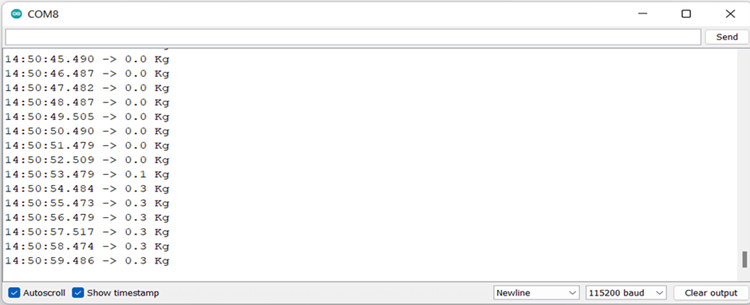
\includegraphics[width=1\textwidth]{Chapter 3/Weight Sensor/LoadCellTestTerminal.png}
    \caption{Load Cell Terminal}
    \label{fig:lcterminal}
\end{figure} 

To test the load cell, it was connected to a terminal and the weight values were printed in the serial monitor.
As expected, when nothing was placed on the load cell, the value was 0kg.
When a 270g weight was placed on the sensor the output value was rounded to 0.3kg whereas a 100g weight output 0.1Kg.
When both items were placed on the senor the combined weight was correctly 0.4kg.

\begin{figure}[H]        
    \centering
    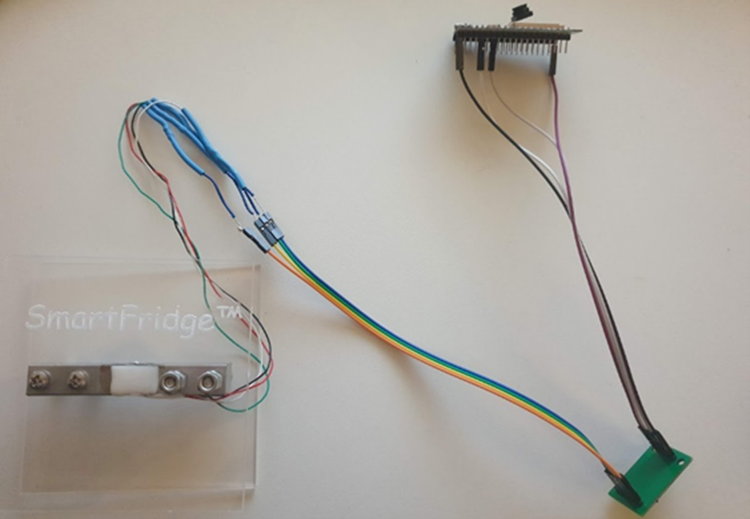
\includegraphics[width=1\textwidth]{Chapter 3/Weight Sensor/WeightSensorWiredImage.png}
    \caption{Load Cell Fully Wired}
    \label{fig:lcwired}
\end{figure} 

It was found that the mass value takes about 2 seconds to stabilise therefore when the code is added to the repository, there should be a 2 second delay between measurements.
When the code was added to the repository, the code in the loop was put in a function which gets the weight of the sensor when called and the setup function was put in a function to setup the sensor.
This meant the entire operation of the weight sensor could be controlled with 2 function calls.

\subsection{ESP-32 Wrover Dev-Board Camera [IB]}

To scan the item, a camera must be placed within the door to detect incoming and outcoming items.
One of the main reasons the Esp-32 Wrover Dev-Board was chosen was due to it having a camera connected directly to a microprocessor.
Typically, external esp cameras require over a dozen connections to the microprocessor.
This would greatly increase the complexity of the build and could result in extensive soldering which could lead to errors such as poor connections and information loss.
Also, by having the camera connected directly to the board, there is now more pins available to connect the other components to.
The board contains 2 cores, this allows the processor to run multiple tasks at the same time instead of unnecessarily waiting.

There is an Arduino IDE library called 'esp\_camera.h' which contains functions that control the operation of the camera.

\begin{figure}[H]        
    \centering
    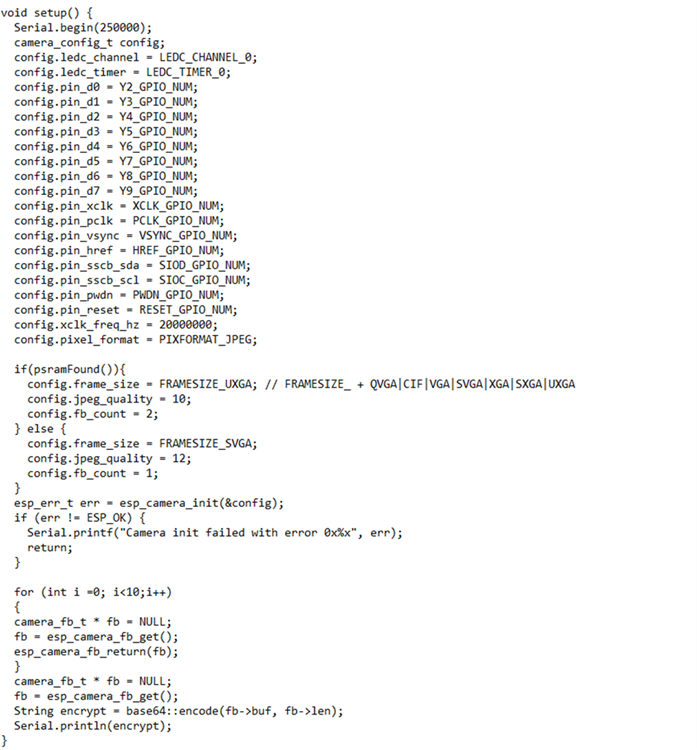
\includegraphics[width=0.75\textwidth]{Chapter 3/ESP-32 Wrover Dev Board/ESP32Camera.png}
    \caption{ESP Camera Code}
    \label{fig:espcamcode}
\end{figure} 

A config object needs to be created so that the pins can be assigned.
Given that the camera is connected directly to the board, the pin configuration is defined on the board's datasheet.
The quality of the jpeg is determined by the member variable jpeg\_quality.
It is crucial that the jpeg quality is maximised so that a clear image is sent to the OpenCV program to read the barcode.
To take a photo the buffer variable fb must be set to null.
The function esp\_camera\_fb\_get() is used to take the photo and store in fb.

The image will be packaged with the weight and the ON/Off state and sent via serial to the raspberry pi to be processed.
A major issue that was faced was that jpeg images can't be sent over the serial to the raspberry pi, only Integers, strings etc.
To fix this issue, a base64 encoder was used to encode the image as a base64 string.
This string can be sent via the serial and decoded back into a jpeg in the raspberry pi.
A base 64 string is around 170 thousand characters and can be captured and sent via serial in around 1 second.
Considering the weight sensor takes a similar amount of time, threading will be easier as they can both start and finish their tasks simultaneously and be sent together without excess delay.

\begin{figure}[H]        
    \centering
    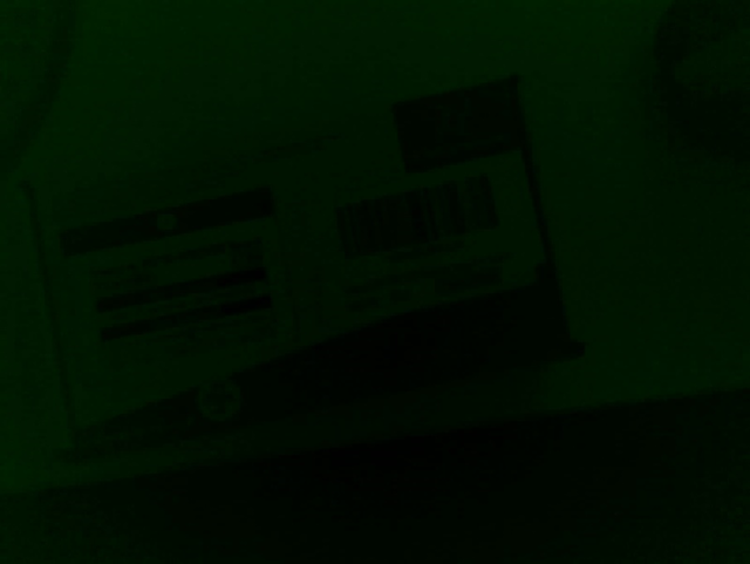
\includegraphics[width=1\textwidth]{Chapter 3/ESP-32 Wrover Dev Board/ESP32Picture.png}
    \caption{First Picture from ESP Camera}
    \label{fig:espcamfp}
\end{figure} 

When the code was uploaded to the board, the program would crash due to there being no more room for the buffer.
At first it was believed that this error was because the size of the buffer was too big.
To reduce the file size, the jpeg quality was reduced by making the variable jpeg\_quality smaller.
Even after this change, the same error occurred.
It was then found that the issue wasn't the size of the buffer but the fact that it wasn't reset after the photo was taken.
This was causing the memory to leak.
The function esp\_camera\_fb\_return(fb) was used after each photo to return the buffer and the jpeg quality was changed back to the maximum value.

Once this error had been fixed a 170 thousand character string was printed to the serial whenever a photo was taken.
The next problem faced was that the photo which was taken was very dark and had a green filtered look.
This can be seen in figure 10.

At first it was thought that this issue was due to data loss by encoding and decoding an image in base64 however it was found that when using base64 on random jpeg images from the internet, this green distortion wasn't found.
Typically, this camera module is used to stream 30fps video to a server, therefore it goes against the original function of the module to take isolated photos.
After extensive research it was found that multiple images need to be taken to “warm up” the camera before saving the final photo.
To do this, a ten iteration for loop was added before the final capture to take and delete “warm up” photos.
This process effectively simulates the first 333ms of a video recording as the camera begins operation.
After integrating this into the code a photo was output which no longer had a green look to it.

\begin{figure}[H]        
    \centering
    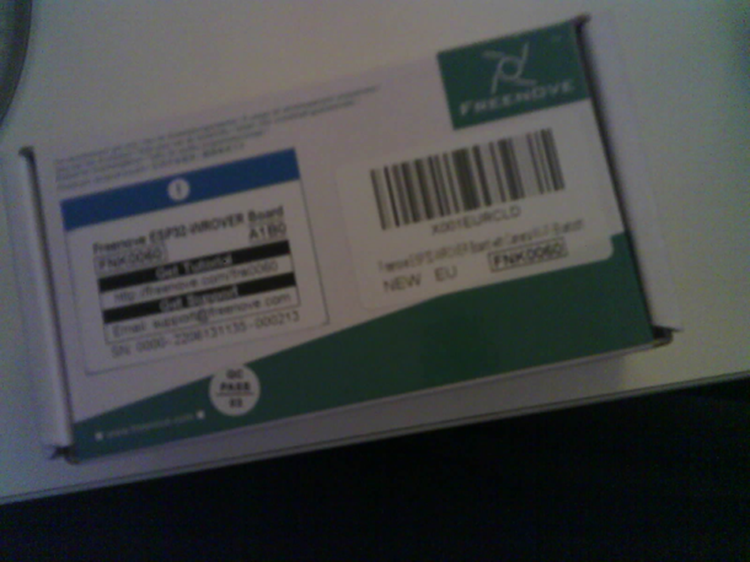
\includegraphics[width=1\textwidth]{Chapter 3/ESP-32 Wrover Dev Board/ESP32BetterPicture.png}
    \caption{Better Picture from ESP CAM}
    \label{fig:espcambetterpic}
\end{figure} 

The number of warm up photos taken was altered to identify the effect and it was found that 10 is the number where the quality doesn't get noticeably any better.

The base64 image was sent to the raspberry pi to use the OpenCV code to detect the barcode on the image.
Unfortunately, the code was unable to detect the barcode in the image.
Dozens of images were tested, each with different angles, distances and focuses and in not one example was the program able to detect the barcode.
It was concluded that the camera resolution wasn't high enough to accurately detect the thin lines of the barcodes.
Given that the resolution of the camera was already maximised, there was very little that could be done to improve it.
Lots of time could be spent trying to find the perfect conditions to take the photo however in the final product the camera will be fitted within the fridge therefore there will be no control over things like angle and distance without heavily disrupting the user experience.

With time and the customer in mind, it was decided that the esp camera was no longer going to be used.
Instead, a web camera will be connected directly to the raspberry pi.
This will ensure a high-quality image is sent to the OpenCV program as well as simplify the product by not needing to encode and decode the image across the serial.
When tested, the program was able to accurately detect the barcode.
Given that the rest of the hardware was built around this esp board, it will continue to be used however the camera module will be disconnected.

\subsection{Buzzer [IB]}

Once the fridge door is open, a timer will start.
Once this timer has reached a certain time a buzzer will activate to remind the user to shut the fridge door.
The 85dB Panel Mount Continuous Internal Piezo Buzzer will be used due to its small size and its low price.
The tone of the buzzer is determined by the frequency set via the esp pin.
Two connections are required for this buzzer, a pin connection and ground.

\begin{figure}[H]        
    \centering
    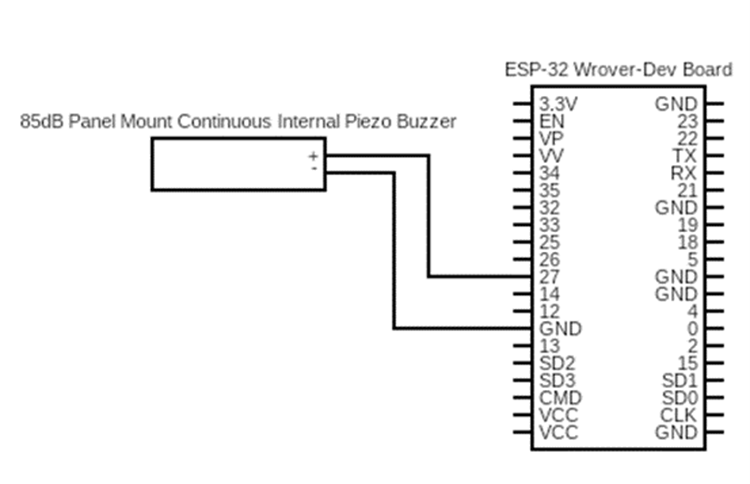
\includegraphics[width=1\textwidth]{Chapter 3/Buzzer/BuzzerCircuitDiagram.png}
    \caption{Buzzer Circuit Diagram}
    \label{fig:buzzcircuit}
\end{figure} 

The tone will be set to 1kHz and sound on and off every second.
Pin 27 is assigned as an output pin and will send 1 kHz signal to the buzzer using the function called 'tone'.
A 1 second delay will keep the buzzer on using the function called 'delay'.
The buzzer will then be turned off using 'noTone'.
A further delay was added to keep the buzzer off for 1 second before the loop begins again.
When tested, the buzzer produced a loud 1kHz alarm that sounded on and off every second.
After some experimenting, it was found that decreasing the frequency and increasing the delay made the buzzer sound less alarming whereas increasing the frequency and decreasing the delay made the sound from the buzzer sound too irritating to listen to and it therefore might harm the user's experience.
The frequency and delays were kept at 1kHz and 1 second.
The code was then wrapped in a function and added to the repository to be called when the fridge door timer runs out.


\subsection{HAL Sensor [YJ]}

Fridges need to know when the door is open or when the door is closed.
There are numerous ways to do this, a mechanical switch or implementing a HAL effect sensor.
Our Product uses the latter.
All fridges use magnets to create a soft close door feature and to hold the door closed.

\begin{figure}[H]        
    \centering
    
\includegraphics[width=1\textwidth]{Logo.png}
    \caption{Place Holder: Magnet Pic}
    \label{fig:placeholder}
\end{figure} 

The Hall effect switch will turn on in the presence of a south magnetic field on its face or a north magnetic field on the opposite side.
It will turn off when the magnet is not in range.

\begin{figure}[H]        
    \centering
    
\includegraphics[width=1\textwidth]{Logo.png}
    \caption{Place Holder: HAL Code}
    \label{fig:placeholder}
\end{figure} 

We can monitor the sensor readings as shown above, and if there is a change in the state, we know when the door is open or closed.
In our feature, the sensor returns True when the doors are open and False when the doors are closed.



\section{Software}
\subsection{ESP32 Firmware Code[YJ]}

The following sections below will provide the reader with knowledge of Firmware code.
By doing so, the reader will understand how all the pieces of software fit together and the intensive testing done to test the features.
Throughout this section, the reader will learn how the raw sensor values received help produce meaningful behavior on the product side.
I will discuss the knowledge and skills I gained during this process.

The hardware controller chosen for this project was from the ESP-32 family.
The system was architected to have its operating system using FreeRTOS.
The system uses software timers to calculate how long the door has been kept open.
The calibrated sensor values, the door and alarm states are packaged as a JSON document and transmitted to the Raspberry Pi through serial communication.
The code development and integration started after proof that the individual sensors would behave and operate as designed during our initial testing.
The tasks and timers created matched the design specification that was agreed upon by the group.

Attached below is the system-level diagram for the microcontroller.
The weight values are stored and used as a comparison again for the next reading to determine the object's direction.

\begin{figure}[H]        
    \centering
    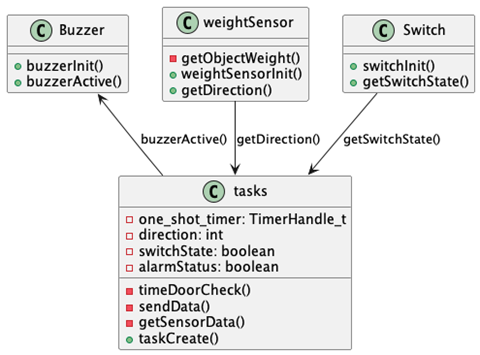
\includegraphics[width=.66\textwidth]{Chapter 4/Firmware Code ESP32/ESP32ClassDiagram.png}
    \caption{UML for System Machine}
\end{figure} 

\subsubsection{RTOS [YJ]}

RTOS is commonly known as Real Time Operating System.
It is an operating system with key features such as predictability and determinism.
An operating system is a computer program that supports a computer's fundamental functions and provides services to other programs that run on the computer.
RTOS creates tasks based on priority while keeping the context switching to the minimum.
Context switching is storing the current state of the thread that is resumed later at a different point in time.
It allows multiple processes to share the same CPU, which is the core feature of multitasking operations.
\cite{RTOS:1} \cite{RTOS:2}

The RTOS kernel used in this project is FreeRTOS.
FreeRTOS is small and light to run on small microcontrollers.
It is preferable because most microcontrollers do not have enough RAM and flash storage.
FreeRTOS also makes it easy to connect IoT( Internet Of Things) devices to the AWS( Amazon Web Services )services by Amazon.

Espressif Systems is a privately held fabless semiconductor company.
They provide wireless communications and Wi-Fi chips in mobile devices and the Internet of Things applications.
The Smart-Fridge uses the ESP-32-Wroom-32 microcontroller.
The Software Development Kit provided by Espressif has a different version of FreeRTOS with slight variations from the vanilla FreeRTOS natively used.
It allows us to freely call the API functions of the FreeRTOS without having to download or include any library.

For this project, to keep in mind simplicity and rapid prototyping and testing requirements, I have designed the tasks system as follows.

The threads generated using "xTaskCreate" are getSensorData and sendData.
The data shared between these two tasks is handled through a message queue buffer.
It prevents memory corruption where one thread reads while the other writes simultaneously.
This message queue is made by "xQueueCreate".
The data collected in the "getSensorData" task is sent to the message queue by "xQueueSend", and the "sendData" receives the latest data on this message stack by “xQueueReceive".

I initially struggled to get the tasks to run on the microcontroller as I was dealing with dangerous memory access errors.
After reading the documentation provided on the FreeRTOS website, I was able to debug the solution and solve the issue.
To understand the timing difference and priority between the two threads, I wanted to provide the lowest delay possible for the sensors so that the system would not miss any event that occurred.
The delay on the data transfer is at 1 second.
It gives time for the processor to average the raw readings and provides accurate results.

\subsubsection{Software Timer [YJ]}

A software timer is a function that executes after a pre-defined period.
The task called after the timer should perform simple short tasks such as toggling a state or changing a variable so that the system does not hang in this state or accidentally trigger the watchdog and reset the microcontroller.
The function executed by the timer is called the timer's callback function.

As the name suggests, the software timer calculates the time by the operating system and does not rely on the hardware.
The advantages of the software timer are that they do not add any processing overhead and take up minimal space on the applications binary.

In our application, we first declare the software timer and define its duration along with if it is a timer to be repeated automatically by the system or manually triggered by a set condition.
The Timer callback function changes the state of the "alarmState", which activates the buzzer till the door of the fridge is closed.

\subsubsection{ESP-Pi Communication [YJ]}

The ESP-Firmware must communicate with the Raspberry Pi.
The messages to the pi are on an agreed-upon pre-defined data table mentioned below.
The table mentioned below tells the Pi the current state of the fridge regarding the alarm, door and objects entering and leaving the fridge.

% Please add the following required packages to your document preamble:
% \usepackage{longtable}
% Note: It may be necessary to compile the document several times to get a multi-page table to line up properly
\begin{longtable}[c]{|l|l|l|l|}
    \caption{ESP to PI Comms}
    \label{tab:yohan}\\
    \hline
    Number &
      Message &
      Value &
      Purpose \\ \hline
    \endfirsthead
    %
    \endhead
    %
    1 &
      DIRECTION\_NO\_CHANGE &
      0 &
      \begin{tabular}[c]{@{}l@{}}Object weight leaving and\\ entering the fridge is the same\end{tabular} \\ \hline
    2 &
      DIRECTION\_LEAVE\_FRIDGE &
      1 &
      \begin{tabular}[c]{@{}l@{}}Object left the fridge as weight\\ drops to 0\end{tabular} \\ \hline
    3 &
      \begin{tabular}[c]{@{}l@{}}DIRECTION\\ \_ENTER\_FRIDGE\end{tabular} &
      2 &
      \begin{tabular}[c]{@{}l@{}}New Object enters the fridge\\ as weight is different to\\ previous object\end{tabular} \\ \hline
    4 &
      DOOR\_OPEN &
      1 &
      \begin{tabular}[c]{@{}l@{}}HAL sensor returns HIGH state\\ hence door is open\end{tabular} \\ \hline
    5 &
      DOOR\_CLOSE &
      0 &
      \begin{tabular}[c]{@{}l@{}}HAL sensor returns LOW as\\ magnet is in contact with the\\ sensor hence door is closed\end{tabular} \\ \hline
    6 &
      ALARM\_ACTIVE &
      1 &
      \begin{tabular}[c]{@{}l@{}}Door kept open longer than\\ predefined safe limit hence\\ ALARM is activated\end{tabular} \\ \hline
    7 &
      ALARM\_INACTIVE &
      0 &
      \begin{tabular}[c]{@{}l@{}}Door kept open longer than\\ predefined safe limit hence ALARM\\ is activated\end{tabular} \\ \hline
    \end{longtable}

Three states tell the direction of the object, they are no changes in the path, an item is leaving the fridge, and an item is entering the smart fridge.
The other values are booleans that tell the Pi if the door is open and if the alarm has been raised for the door being open for too long.

Communication between the ESP32 and the Pi happens through the UART protocol.
A JSON packet is packaged with the three states, as seen below and sent to the Pi.
JSON serialisation is favourable to transferring data as the system can send all the information in a single message packet.
The drawback of this system is that there is only one-way communication between the two boards using one UART serial port.

The fix is to utilise the second set of UART pins on the Esp32 if the ports are unused.

The ArduinoJSON library determined how the messages were packed on a JSON document and sent via the serial port.
The JSOC document requires a key that maps to a value.
I struggled with sending the JSON document through the second UART port on the development board.
The board's documentation sheet mentioned that there were two sets of UART pins enabled on the development board but only able to transmit and receive.
I tested this by connecting the pins to an Arduino UNO board running a deserialisation script that printed NULL but printed the values using the default pins for Transmit and receives on the ESP-32 board.

\begin{figure}[H]        
    \centering
    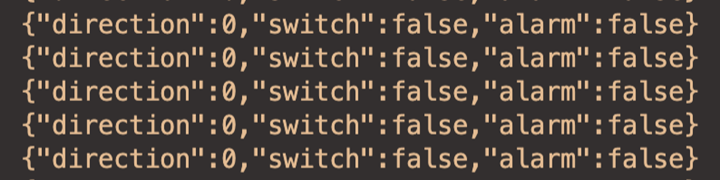
\includegraphics[width=1\textwidth]{Chapter 4/EspToPiCommunication/JSONPACKET.png}
    \caption{JSON Packet Sample}
\end{figure} 

\begin{figure}[H]
    \begin{subfigure}{.5\textwidth}
      \centering
      
\includegraphics[width=.8\linewidth]{Logo.png}
    \end{subfigure}%
    \begin{subfigure}{.5\textwidth}
      \centering
      
\includegraphics[width=.8\linewidth]{Logo.png}
    \end{subfigure}
    \caption{PLACEHOLDER: Serialisation and Deserialisation Scripts}
\end{figure}

\subsection{Raspberry Pi Overview [AW]}

As mentioned in the system overview, the Raspberry Pi receives a JSON packet from the ESP-32 which will alter the response of the Pi and change the data to be sent to the database.
The JSON itself is discussed at further length in the Pi Serial Input section.
The Raspberry Pi also handles the camera, the computer vision calculations, and the networking to the database.
These are the features that will be explored in this section, starting with the different computer vision methods utilized.

\subsubsection{Pi Object and character recognition [IB]}

There are two tasks that utilize object and character recognition.
The first one is the expiration date which is implemented using a OpenCV and a python library and the output gives the characters, in this case the numbers of the expiration date.
The second task is to take an image of the product and using an already trained model, the product will be classified and return its class.
	

\subsubsection{Expiration Date - Character Recognition [IP]}

The implementation of the expiration date recognition requires loading an image and then processing it to be able to use a function that will extract the digits detected.
The function that identifies and extracts the characters comes from a library called PyTesseract.
PyTesseract is a python tool used for optical character recognition, that recognizes and extracts characters on an image [pypiPytesseract].
The code written can be found in a repository on github.
In the code implemented, the image is loaded using the OpenCV library's image read function (imread) and then converted from BGR to RGB channel ordering, again using an OpenCV library function.
The function named image\_to\_string from PyTesseract tool is then called which takes in the rgb image and stored in a variable.
The variable holds the text of the characters extracted and is the output of the code.

A virtual environment was used to run the code in which the PyTesseract was installed, as well as the rest of the necessary libraries such as OpenCV.

The PyTesseract tool is an engine that functions by following a series of stages that include finding and nesting the outlines, organising into text lines, and then the recognition follows using an adaptive classifier.
The first step is inspecting the nesting of the general outlines as well as the smaller ones.
The outlines are assembled into objects which are then organised into text lines.
The next step includes testing whether the test lines are fixed pitch, and the text lines are divided into words according to the spacing between them.
Recognition of the text is the next process that takes place, which is done by firstly recognising each word and then passing it into a classifier.
The process is repeated for the case where the classification didn't successfully recognize words [TesseractOverview].

The performance of the expiration date detection was tested using images initially with just numbers and then of more complicated images, meaning the products with expiration date on them.
In the images with just numbers taken from google, the average performance was satisfactory as the output of the code returned the number that was embedded on the image.
The images that contained the products had a poorer performance as the majority of the images were not as clear regarding the intensity of the image and the shape of the characters.
Initially, this was a major drawback as other than the images used for testing from the internet, images were captured from the ESP32 camera but failed the tests, as they were very blurry and unfocused.
This was discussed with the rest of team, and it was decided that the ESP32 camera wouldn't be used, and a web camera would replace it.
Images captured from the webcam were then tested and had a much-improved performance.
The lighting when the image is captured is highly important as it can zero the possibility of the function's ability to read and extract the characters.

\subsubsection{Product detection – Object recognition [IP]}

The product detection was implemented by training a convolutional neural network using a public dataset.
The dataset included images of grocery items of 43 different classes, that included mainly vegetables and fruits, as well as other products.
There are a total of 5,571 images that are used for training, testing and validation sets.
The model is trained on this dataset, and then the image captured from the fridge is tested on the model.

\subsubsection{Background theory on design implementation [IP]}

A convolutional neural network (CNN) was used as it is considered as one of the most efficient algorithms for image classification.
In this case, a simple architecture of a CNN was designed with the addition of using a pre-trained model, using transfer learning.
A model consists of layers in which the training of the data takes place.
The first layers of a model train the data on more generic features such as shapes, edges, and colours, whereas the higher layers learn more complex and specific features.
A more efficient way to train the data would be to use a model that has been pre-trained in the more generic task features and complete training only for the more complex task features.
The pre-trained model used is the VGG16 architecture which consists of 16 layers that hold the learnable parameters (weights), 3 convolutional layers, 5 max pooling layers and 3 dense layers, in total 21 layers [VGG16overview].
The convolutional layers use filters, or kernels with the purpose of performing the convolution operation on the input and give an output of a feature map that comprises the features detected.
The max pooling layers perform an operation that takes the maximum value of a specified region on the feature map with the aim to reduce its dimension.
Lastly, the dense layers contain the neurons that are connected to the ones in the previous convolutional layers with the aim to perform the classification.
The architecture of the VGG16 architecture is shown in figure [update].

\begin{figure}[H]        
    \centering
    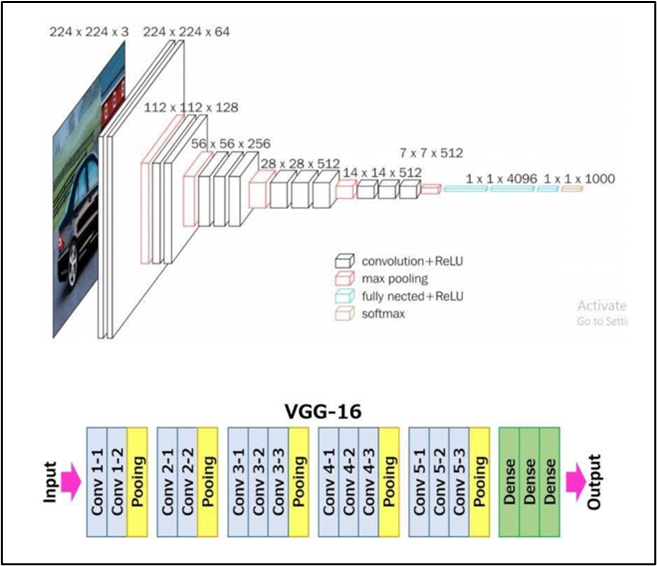
\includegraphics[width=.66\textwidth]{Chapter 4/CNN/VGG-16.png}
    \caption{VGG16 Architecture}
    \label{fig:cnn}
\end{figure} 

\subsubsection{Pre-processing of the dataset [IP]}

The dataset that is used as the input to train the model required processing into the appropriate train, test, and validation sets.
The training and validation sets contain the data based on which the model is trained on, and the test set contains the data used to test the performance of the trained model.

The dataset consists of 3 main categories, which were vegetables, fruits, and packages.
Within each of these three categories, there were subcategories which resulted in 43 classes in total from all categories.
The goal of the classifier is to classify what the product is, so between these 43 classes, and not to which generic group/category they belong to.
Therefore, the 3 categories were removed, and all 43 classes were put under the same folder, for all three training, testing and validation sets.
The dataset had already completed the splitting between the sets.
The dataset was taken from a repository \cite{dataset} and was used for a research paper.

\subsubsection{Model architecture [IP]}

For the model architecture, as mentioned before in the background theory, a VGG16 pre-trained model was used for which the features learned were stored in some filed, known as the bottleneck files.
The bottleneck files were created for all three tests (training, testing and validation) and were loaded to be used as the according data.
The labels for each class were generated using the ImageDataGenerator, a TensorFlow pre-processing function and were transform the data to a binary class matrix before passing it to the model.
After the data and the labels for each set were prepared, the model architecture was designed.
A sequential model was initialised, as the following layers used are in a linear stack.
The first layer, which is a Flatten layer, contains the data that has been taken from the bottleneck files.
The dense layers contained the activation function that determined the values that the neurons would hold.
The dropout layers randomly neutralise some neurons during the training with the aim of preventing overfitting, meaning the model not being able to generalise and only being able to accurately predict the already trained data.
A SoftMax activation function was used to compute the probabilities for the output for all the classes.
After the model's architecture design, the data was fitted in the model and the training occurred.
A batch size and number of epochs was specified.
After the training, the weights of the model were saved, and an accuracy and loss score were printed.


\subsubsection{Expiration Date Evaluation [IP]}
The performance of the expiration date detection was tested using images initially with just numbers and then of more complicated images, meaning the products with expiration date on them.
In the images with just numbers taken from google, the average performance was satisfactory as the output of the code returned the number that was embedded on the image.
The images that contained the products had a poorer performance as the majority of the images were not as clear regarding the intensity of the image and the shape of the characters.
Initially, this was a major drawback as other than the images used for testing from the internet, images were captured from the ESP32 camera but failed the tests, as they were very blurry and unfocused.
This was discussed with the rest of team, and it was decided that the ESP32 camera wouldn't be used, and a web camera would replace it.
Images captured from the webcam were then tested and had a much-improved performance.
The lighting when the image is captured is highly important as it can zero the possibility of the function's ability to read and extract the characters.

\subsubsection{Product Detection Evaluation [IP]}
For the testing part of the product detection, two functions were created, one to read the image and another to predict the class of the image based on the model.
The first function that reads the image, converts it to an array of values and normalises by dividing values by 255 for the computation to be faster.
The second function loads the trained model and weights and stores them in a variable named reconModel, for reconstructed model.
After all the possible classes are defined, the image reading function is called and then the image is used to perform the prediction.
After testing the model with a test set, the model had a poor performance, but this was expected as there was a class imbalance within the training set.
This is not something that can be handled within the scope of this project, as it would require adding images and labelling them accordingly to their class.
Therefore, a better architecture of the model was attempted to be completed for a newly trained model that would take into consideration trying to reduce overfitting.
Additionally, the framework used was TensorFlow, and the process of using the pre-trained model to predict the class of the image was taking longer than expected, hence another approach was changing to PyTorch framework.


For the testing part of the product detection, two functions were created, one to read the image and another to predict the class of the image based on the model.

\subsubsection{Barcode Detection [JG]}

An important feature of the smart fridge was to identify the products placed inside it.
One of the ways in which we sought to achieve this was using a barcode detection system.
The idea for this was to find and decode barcodes found within the image received from the camera.
This would then be sent to the server to identify the product.
The code for barcode detection would be written in Python, using the OpenCV library to search the image for the barcodes, as well as any other libraries required to efficiently complete this task.
It was decided that we would use an 'off-the-shelf' algorithm as inspiration which we could later adapt to suit our needs.
Overall, three algorithms were tested in order to arrive at the best option for our product.
They were tested using three images containing barcodes.

The first image was the back of a notebook.
The idea was that this image would be the simplest as the barcode would be located on a flat, smooth surface.
A chosen algorithm would be expected to correctly detect and decode this barcode.
The second image was a barcode on a jar.
This image was intended to be more challenging as the surface of the barcode, although smooth, was no longer flat as it followed the curve of the jar.
A chosen algorithm would again be expected to detect this barcode, albeit with a lower success rate.
The third was of a barcode on a bottle.
This image was selected to be the most challenging of the three as the surface of the barcode was neither flat nor smooth.
A chosen algorithm was not required to successfully detect or decode the barcode in this image as its purpose was mainly to test the limits of each algorithm.

The first algorithm [Detecting Barcodes in Images with Python and OpenCV] only detected barcodes and did not decode them.
However, this was chosen as a starting point as [1] explained the workings of the algorithm clearly and in detail.
The algorithm begins by converting the image to greyscale using the Sobel function found within the OpenCV library.
From this the x and y gradients from the Scharr operator are subtracted which gives the regions of the image which have the largest horizontal gradients and the lowest vertical gradients as these are most likely to contain barcodes within them.
The next step was to blur the image and to threshold the image, so that, pixels in which it was decided that a barcode is unlikely to be, could be set to black and pixels where a barcode was likely to be, could be set to white.
This would reduce the noise of the image in order to make the following steps easier and more effective.
The code up to this point is shown in the image below.

\begin{figure}[H]        
    \centering
    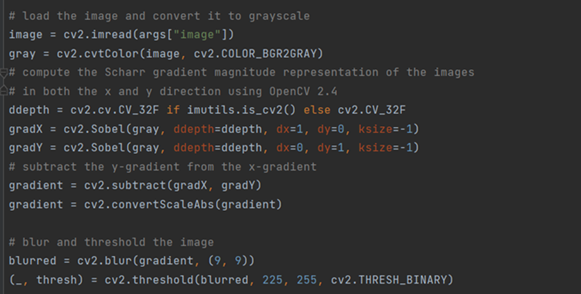
\includegraphics[width=0.5\textwidth]{Chapter 4/Barcode Detection/Figure1.png}
    \caption{Greyscaling and Blurring Code}
    \label{fig:bc1}
\end{figure} 

However, this previous step would also create gaps within the actual barcode.
Therefore, it was necessary to perform morphological operations using a rectangular kernel, once to close gaps between bars in the barcodes, and again to close any gaps within these bars.
These were then followed by four iterations of dilations which aimed to remove any remaining gaps in the barcode.
The next step was to find the largest contour in the image as this is likely the region which contains the barcode.
The code for this is shown below.

\begin{figure}[H]        
    \centering
    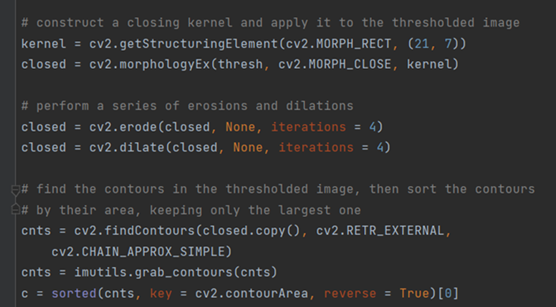
\includegraphics[width=0.5\textwidth]{Chapter 4/Barcode Detection/Figure2.png}
    \caption{Gap Closing and Contour Finding Code}
    \label{fig:bc2}
\end{figure} 

This algorithm's performance on the three test images exceeded expectations.
It was able to correctly detect the barcodes on both the notebook and the jar, however, the algorithm was also able to detect the barcode on the bottle.
Therefore, the only disadvantage of this algorithm was the missing functionality for decoding barcodes.
Due to the quality of the results, this functionality was added and tested.
Unfortunately, it was not possible for this to be implemented in a way that kept the results of the barcode detection within the time that was allocated for this algorithm.

The second algorithm [Barcode-Reader] added onto the first in that it included functionality for both detecting and decoding barcodes.
The sections of code dedicated to detecting the barcodes were very similar as the same method was used, with most differences being due to the use of different libraries.
However, the code for decoding the barcodes was new and therefore, the most interesting section.

As with detecting the barcode, the first step to reading the barcode was to convert the image to greyscale.
The image was then thresholded in order to identify the individual bars within the barcode.
Following this, a similar method to the previous algorithm is used to remove gaps from the barcode.
The code for this is shown below.

\begin{figure}[H]        
    \centering
    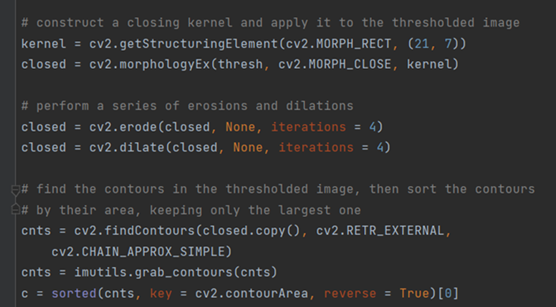
\includegraphics[width=0.5\textwidth]{Chapter 4/Barcode Detection/Figure3.png}
    \caption{Greyscaling, Thresholding and Cleaning Code}
    \label{fig:bc3}
\end{figure} 

Following this the algorithm is then able to extract the binary code from the barcode.
This is done using a separate function within the program, getBinary().
This function works by first calculating the exact boundaries of the barcode.
These are then used to iterate over the barcode as the program finds the average value of the pixels in each bar.
Then, if the average value is high, the bar is read as a '1', otherwise, the bar is read as a '0'.
In the decodeBarcode() function, the barcode is then converted from binary into the appropriate number.
The code for this is shown below.

\begin{figure}[H]        
    \centering
    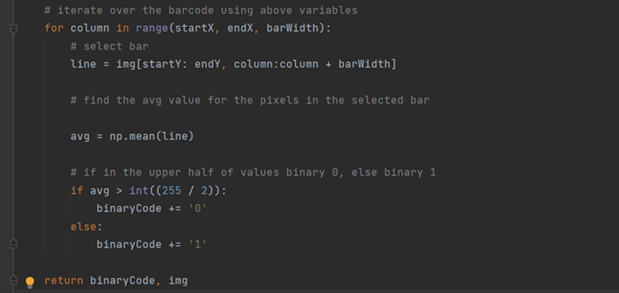
\includegraphics[width=0.5\textwidth]{Chapter 4/Barcode Detection/Figure4.png}
    \caption{Binary Extracting Code}
    \label{fig:bc4}
\end{figure} 

This algorithm's performance on the test images fell below expectations as it failed to either detect or decode the barcode in any of the three images.
It was suspected that there may have been an error in the code which caused this.
Therefore, the algorithm was tested using the test image provided by [Barcode-Reader].
When tested with this image the algorithm functioned properly, detecting the barcode and decoding it correctly.
In order to test whether one section of the code was working worse than the other, the barcode decoding sections of the code were implemented with the barcode detection of the previous algorithm.
However, this did not improve its performance.
Therefore, this algorithm was discarded as an option.

The third algorithm [How to Make a Barcode Reader in Python] also provided functionality for both detecting and decoding barcodes.
However, this algorithm achieved this using the pyzbar library, which was designed for detecting and decoding barcodes.
As a result, the code for this third algorithm is much more condensed and easier to read.
For example, when using the pyzbar library, detecting and decoding a barcode is done with one line of code.
This is shown in the image below.

\begin{figure}[H]        
    \centering
    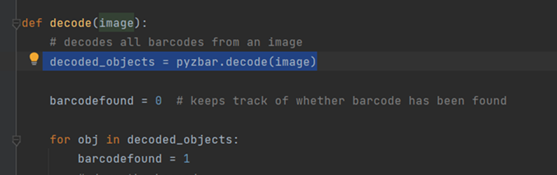
\includegraphics[width=0.5\textwidth]{Chapter 4/Barcode Detection/Figure5.png}
    \caption{Barcode Detection and Decoding Code (highlighted)}
    \label{fig:bc5} 
\end{figure} 

The program then used the glob library to iterate through files of the name “barcode*” where '*' is a number and added them to a list.
From here the program could iterate through the list, decoding the barcodes in each of these images.

This algorithm performed as expected on the tests.
It was able to both read and decode the barcode on both the notebook and the jam.
Despite this, the algorithm was unable to either detect or decode the barcode on the bottle, however, given the challenging condition of that barcode, this was not a requirement for an algorithm to be chosen.
The results for each test are shown below.

\begin{figure}[H]        
    \centering
    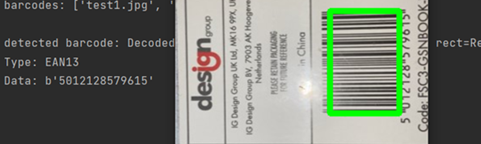
\includegraphics[width=.66\textwidth]{Chapter 4/Barcode Detection/Figure6.png}
    \caption{First Result}
    \label{fig:bc6} 
\end{figure} 

\begin{figure}[H]        
    \centering
    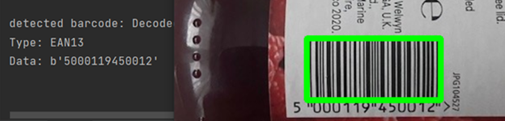
\includegraphics[width=.66\textwidth]{Chapter 4/Barcode Detection/Figure7.png}
    \caption{Second Result}
    \label{fig:bc7} 
\end{figure} 

\begin{figure}[H]        
    \centering
    
\includegraphics[width=.66\textwidth]{Chapter 4/Barcode Detection/Figure8.png}
    \caption{Third Result}
    \label{fig:bc8} 
\end{figure} 


Given the results shown in figures 6-8, this algorithm was chosen for use in our product.
In its original state, the algorithm already satisfied most of the product's needs as it could decode barcodes from an image.
However, it was necessary to add an error message for cases where the barcode could not be decoded.
The first step was to declare a variable, 'barcodefound', at the start of the decode() function and set it equal to 0.
This variable would later tell us whether a barcode had been decoded.
Then, in the for loop within the same function, this variable would be changed to 1.
This worked because the program would only enter the loop if there were items in the decoded\_objects list.
As each item in this list was a barcode, if this list was empty, a barcode was not found within the image and, therefore, the 'barcodefound' variable would remain unchanged.
However, if there was at least one item in the list, 'barcodefound' was changed to 1.
This was then followed by an if statement to check the value of 'barcodefound'.
If this was still equal to 0, a message was printed to the terminal.
This can be seen in figure 8, with the code shown below.

\begin{figure}[H]        
    \centering
    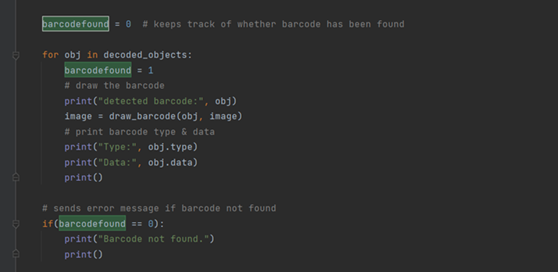
\includegraphics[width=.66\textwidth]{Chapter 4/Barcode Detection/Figure9.png}
    \caption{Error Checking Code}
    \label{fig:bc9} 
\end{figure} 

\subsubsection{Pi Camera [AW]}

A USB camera is plugged into the Raspberry Pi.
Using the OpenCV library to access the camera, pictures can be taken and then analyzed by the previously discussed computer vision methods.
The webcam being used is not perfect but is suitable for a first prototype.
It is unable to have its focus adjusted programmatically so the camera will have to be focused manually when being fitted into the enclosure.

This is fine for now but in the future, it would be appropriate to replace the webcam with a different camera that allows for focus to be adjusted automatically and is more suited to fitting within the housing of a fridge.
By doing this, the reliability of extracting barcodes and expiration dates would increase due to having higher clarity images.

\begin{figure}[H]        
    \centering
    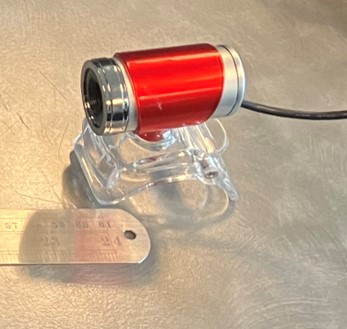
\includegraphics[width=0.5\textwidth]{Chapter 4/Pi Camera/ImageOfWebcam.jpg}
    \caption{Webcam}
    \label{fig:webcam} 
\end{figure} 

The images are stored in a bitmap image file, known as BMP for short.
This is done to maintain a high-resolution image as opposed to the JPEG file format.
Figure [IMAGE OF PI BARCODE] shows an image from the camera on the raspberry pi.

Since the original design intended for an ESP32 camera to be used, the webcam was a backup idea that had to be utilized with the time left.
Fortunately, the Pi is perfectly suited to handling the camera since the open cv library is already a requirement and the goal was to transfer the image from the ESP-32 to the Pi regardless.
Ultimately, it has increased the complexity of the wiring while decreasing the complexity of the ESP-32 and Raspberry Pi code.

\begin{figure}[H]        
    \centering
    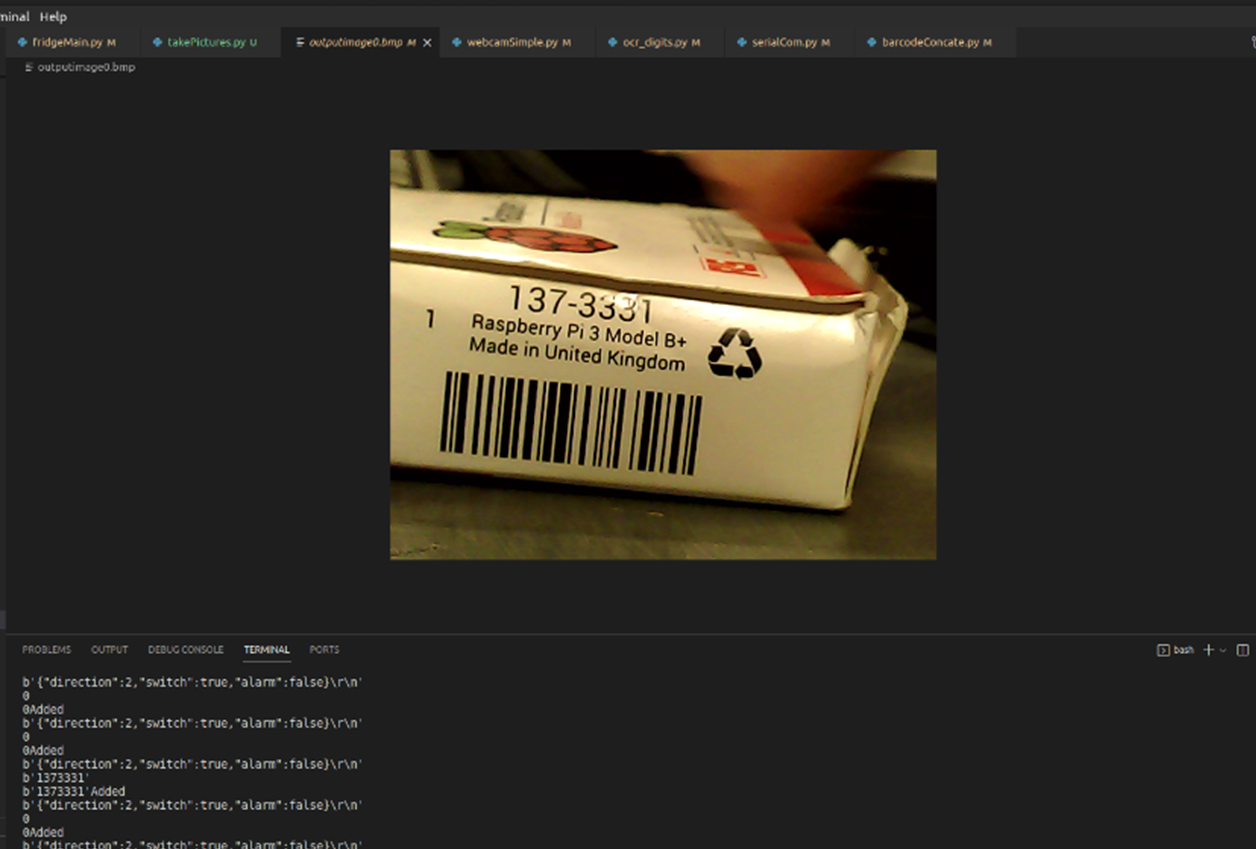
\includegraphics[width=.66\textwidth]{Chapter 4/Pi Camera/PiBoxTakenByCamera.png}
    \caption{Picture from Webcam}
    \label{fig:webcampic} 
\end{figure} 

In figure [FIGURE IMAGE OF RASP PI BOX] a picture taken by the webcam of the Raspberry Pi box barcode can be seen.
In the terminal the byte value of b'1373331' is detected which matches the number written on the box.

\subsubsection{Pi Serial Input [AW]}

To communicate between the ESP-32 and Raspberry Pi, the serial RX and TX pins are connected.
As seen on the pinout [RASPBBERRY \_PI\_DOCUMENTATION\_REFERENCE], the GPIO 14 (TXD) pin is used to transmit data and the GPIO 15 (RXD) pin is used to receive data.

\begin{figure}[H]        
    \centering
    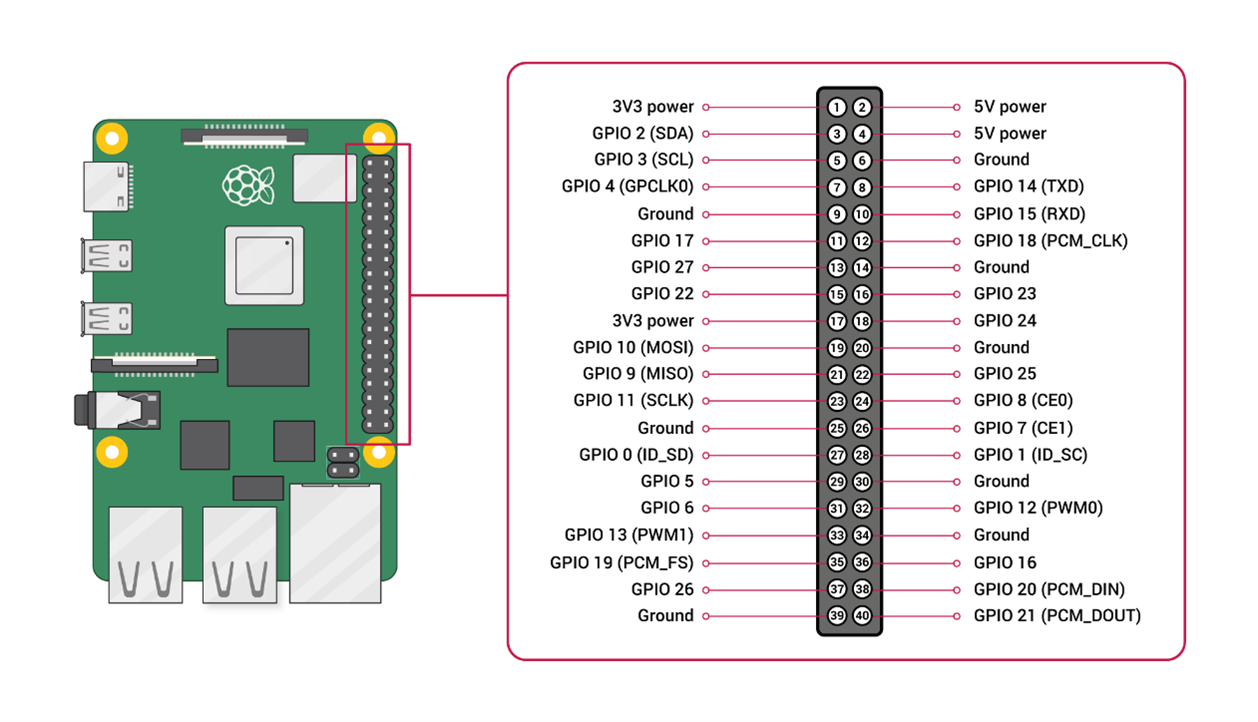
\includegraphics[width=.66\textwidth]{Chapter 4/Serial Input/PiPinout.png}
    \caption{GPIO of the RPI}
    \label{fig:rpigpio} 
\end{figure} 

The information received will be a JSON file containing the status of the door, the direction of movement and if the alarm is sounding.
The JSON format table can be seen in figure [FIGURE NUMBER OF TABLE IN EARLIER SECTION].

The ESP-32 was connected to the Raspberry Pi by using two jumper wires to test if the serial input was functional and as seen in [FIGURE 2, JSONSERIALINPUT]

\begin{figure}[H]        
    \centering
    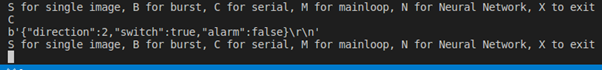
\includegraphics[width=1\textwidth]{Chapter 4/Serial Input/SerialRead.png}
    \caption{Serial Data from ESP}
    \label{fig:rpiserial} 
\end{figure} 

The message received was: “b'{“direction”:2,”switch”:true,”alarm”:false} r n”

Which means that an item is entering the fridge, while the door is open and the alarm is not sounding.

\subsubsection{Pi Communications [ASH]}

For the PI to function it needs to read known items from the database as well as add and remove instances of the items from people's inventory.
Supabase, our back-end, provides a python API to interact with the tables as well as the handle user authentication.
However for ease of use for the Pi Software team multiple functions where designed to simplify and abstract the database commands and manage the database connection the background.
These key functions allow the PI to: retrieve items, add items to inventory, remove items from the inventory and log the user in.

This was done by creating a class that expands on the provided “Client” class from the Supabase python API.
The Client class exposes the same commands as the JS commands and allows the user to perform various actions, however for the RPI side of the communication we are only concerned with interacting with the database.
The commands exposed by Supabase require syntax similar to the SQL command used to drive the database directly, however as mentioned we wanted to abstract these so the SQL commands and code required to package items as JSON have been wrapped into simple commands to getItemID, addItem, and removeItem.
The class also deals with logging the user in, ensuring we can access the users data and subsequently terminating the upon deletions.
All these functions were tested with simple unit test that would login, check items, add items, remove items, get a barcode and logout.

As with the rest of the code base, the communication section was created entirely separately to the main code base meaning that the initial structure was rather different and integration was required.
These changes were later unified in the code refactor.
After this refactor the database code worked well with the rest of the code base, and, as the API is similar in python and JavaScript, the experience of writing this code was easily transferred to creating the App.

\subsubsection {Pi Integration [AW]}

The main bulk of integration is sitting down with the team members who worked on their individual sections while moving the python code to the Raspberry Pi environment.
This ensures that the transition is smooth and that issues are solved as quickly as possible.

% Please add the following required packages to your document preamble:
% \usepackage{longtable}
% Note: It may be necessary to compile the document several times to get a multi-page table to line up properly
\small
% Please add the following required packages to your document preamble:
% \usepackage{longtable}
% Note: It may be necessary to compile the document several times to get a multi-page table to line up properly
\begin{longtable}[c]{|l|l|l|}
\caption{Overview of Python Libraries}
\label{tab:libraries}\\
\hline
Module/Library &
  Section &
  Function \\ \hline
\endfirsthead
%
\endhead
%
serial &
  Serial Communication &
  \begin{tabular}[c]{@{}l@{}}Enables Serial communication on\\ the GPIO 14 pin for transmitting\\ and GPIO 15 pin for receiving.\end{tabular} \\ \hline
cv2 &
  \begin{tabular}[c]{@{}l@{}}Barcode, Optical character\\ recognition\end{tabular} &
  \begin{tabular}[c]{@{}l@{}}Cv2 is the Open CV library for python.\\ It lays the foundation for computer\\ vision code in the project as well as\\ the image handling.\end{tabular} \\ \hline
io &
  \begin{tabular}[c]{@{}l@{}}Barcode, Serial Communication, \\ Optical character recognition\end{tabular} &
  \begin{tabular}[c]{@{}l@{}}The io module provides pythons\\ main methods for dealing with inputs\\ and outputs.\end{tabular} \\ \hline
time &
  CNN, Barcode &
  \begin{tabular}[c]{@{}l@{}}The time library is used to add delay\\ during the image processing.\end{tabular} \\ \hline
json &
  Serial Communication &
  \begin{tabular}[c]{@{}l@{}}The JSON library is used to convert\\ the JSON received from the ESP\\  into readable values.\end{tabular} \\ \hline
pyzbar &
  Barcode &
  \begin{tabular}[c]{@{}l@{}}Pyzbar is the library that handles\\ decoding and detecting barcodes in \\ images.\end{tabular} \\ \hline
pytesseract &
  Optical character recognition &
  \begin{tabular}[c]{@{}l@{}}Pytesseract is the library that handles\\ decoding and detecting characters in \\ images.\end{tabular} \\ \hline
pandas &
  CNN product recognition &
  \begin{tabular}[c]{@{}l@{}}The pandas library is used for data\\ analysis.\end{tabular} \\ \hline
numpy &
  CNN product recognition &
  \begin{tabular}[c]{@{}l@{}}The NumPy module allows python\\ to use high level mathematical functions \\ and operate with large multi-dimensional\\ arrays and matrices.\end{tabular} \\ \hline
shutil &
  CNN product recognition &
  \begin{tabular}[c]{@{}l@{}}Shutil allows the python program to \\ do high level operations on files.\end{tabular} \\ \hline
itertools &
  CNN product recognition &
  \begin{tabular}[c]{@{}l@{}}The Itertools module implements \\ functions to increase the efficiency \\ of loops in the code.\end{tabular} \\ \hline
tensorflow &
  CNN product recognition &
  \begin{tabular}[c]{@{}l@{}}The TensorFlow module used to prepare\\ and load data for machine learning.\end{tabular} \\ \hline
keras &
  CNN product recognition &
  \begin{tabular}[c]{@{}l@{}}Keras provides an open-source software\\ library that acts as an interface for \\ TensorFlow.\end{tabular} \\ \hline
sklearn &
  CNN product recognition &
  \begin{tabular}[c]{@{}l@{}}Sklearn (or scikit-learn) features\\ classification, regression, and clustering\\ algorithms to be used with machine learning.\end{tabular} \\ \hline
\end{longtable}

These modules were installed using “pip install” on the Linux environment on the Pi.

Once all the required modules were installed, the code from other group members must be compiled into a main loop to run on the Pi.
On the other hand, each part must be tested individually first.
This was done by creating a simple loop that asks the user which section they want to run.

\begin{figure}[H]        
    \centering
    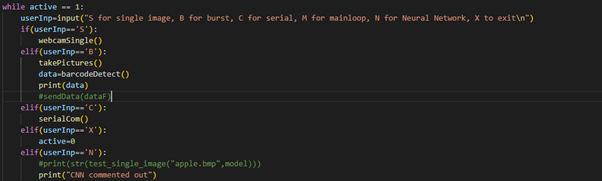
\includegraphics[width=1\textwidth]{Chapter 4/Pi Integration/PiTestLoop.png}
    \caption{Test Loop Code}
    \label{fig:tlcode}
\end{figure} 

As seen in figure \ref{fig:tlcode} the letter S can be input to take a single image and check for barcodes, the letter B to check a burst of images for barcodes, the letter C to test the serial input from the ESP-32, N to test the neural network on an image and X to cancel the program and exit.
This allows the core base functionality to be tested individually before the final implementation.

\subsubsection {Code Refactor [ASH, AW]}

As is inevitable when code is written by many different people, especially when the overall design is not determined before coding begins, our code base was somewhat inconsistent, poorly formatted and used different conventions.
To allows us to iterate and improve the code faster once the different sections, such as the barcode recognition, produce detection, and database iterations, were combined, we took the time to refactor the code into something of a more unified and thought out design.

The first step in the refactor was simply to remove all the unused code (including imports), debug images, and other files left behind from testing.
This alone already made large improvements to readability of the code and allowed us to start making decision like what format to use and how to restructure the code.
Other, more superficial changes, such as setting up a “.gitignore” file to clean up the repository and a requirements file to help set up the requirements on new machines were also made.

After this initial clean-up, we decided to rework the code in a more object orientent style, similar to how the Supabase communication section was initally written.
While doing this we also tried to adopt a more consistent naming scheme for both function and member variables.
This was done in order to unify the style of each of the section, making the code much easier to understand and edit.
We settled for the design seen below in Figure \ref{fig:oocd}, table [x] provides more detail on these member functions and variables.

\begin{figure}[H]        
    \centering
    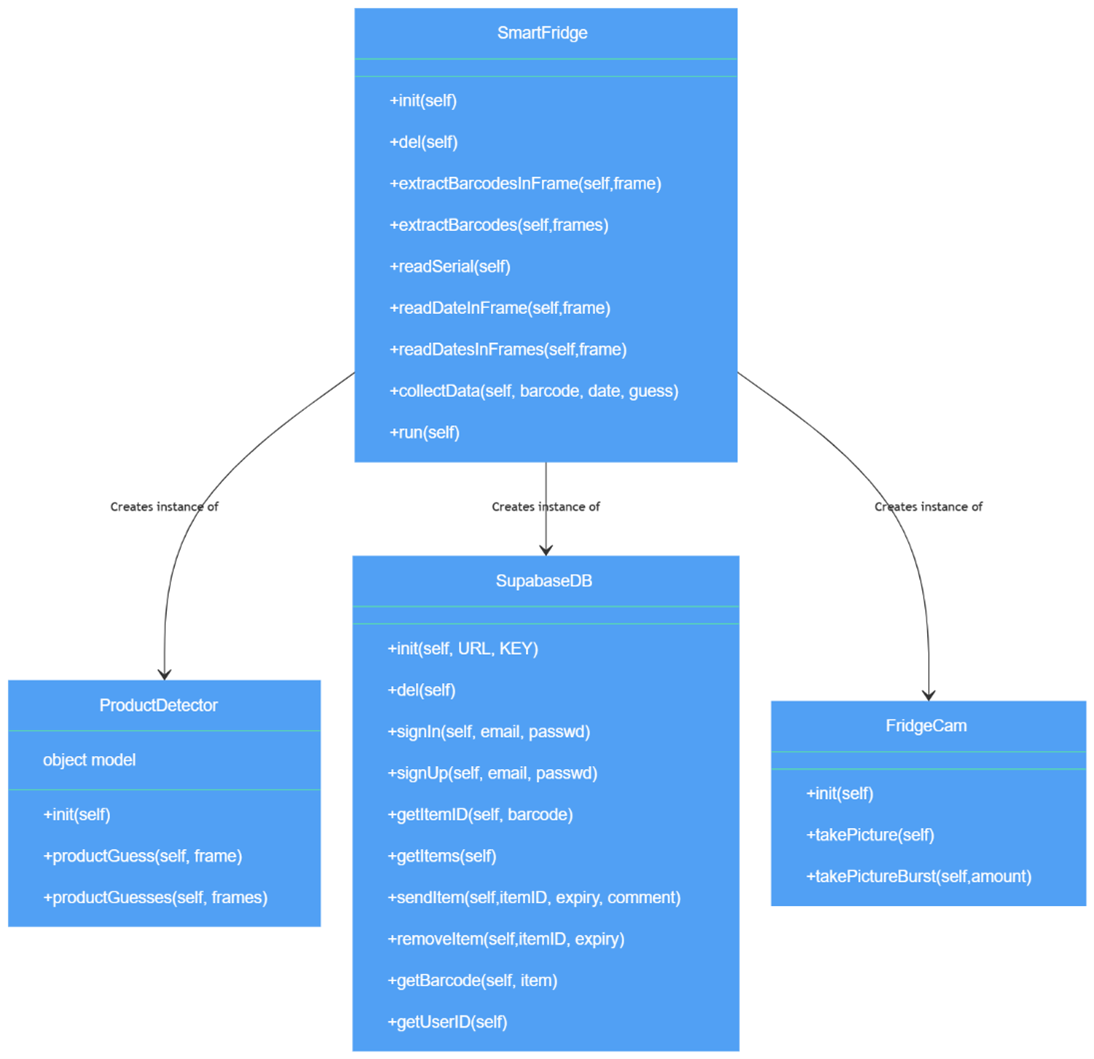
\includegraphics[width=.66\textwidth]{Chapter 4/Code Refactor/Class Diagram.png}
    \caption{Object Oriented Class Diagram}
    \label{fig:oocd}
\end{figure} 

Now the fridges core operations where encompassed in a single object, which itself contains instance of the of objects that simplify and abstract the usage of the CNN product detector, Supabase database connection, and camera.
After this major refactor, we also changed the layout of the python files them selves, placing them in a Smart Fridge directory with an “\_\_init\_\_.py” file which is required for the code to show up as a module.
This allows us to cleanly import all our code into a short run file which will start everything we need for the Smart Fridge's local operation.

While it would have been preferably to have never needed a refactor, this would have slowed initial programming down and would have required many assumption about what choices would be made by other people in the team.
As effort would have been required to integrate the code regardless, doing this refactor allowed us examine our code as well as improve it as we went along.
Testing for this was rather simple, as the end goal was essentially to maintain the same functionality as before, meaning the same test could be run.
This refactor was a success as we managed to improve the code slightly with some optimizations all the while making it much more readable and easier to set-up on another device.

% Please add the following required packages to your document preamble:
% \usepackage{longtable}
% Note: It may be necessary to compile the document several times to get a multi-page table to line up properly
\begin{longtable}[c]{|l|l|}
    \caption{Python Class and Method Overview}
    \label{tab:piview}\\
    \hline
    \textbf{Method/Class} &
      \textbf{Explanation} \\ \hline
    \endfirsthead
    %
    \endhead
    %
    \textbf{ProductDetector Class} &
      \textbf{\begin{tabular}[c]{@{}l@{}}Class that handles the neural network \\ algorithm.\end{tabular}} \\ \hline
    init(self) &
      \begin{tabular}[c]{@{}l@{}}Initializes the neural network by loading\\  in the weights, and  layers of the model.\end{tabular} \\ \hline
    productGuess(self,frame) &
      \begin{tabular}[c]{@{}l@{}}Runs the neural network on the image (frame) \\ passed into the method and returns the name \\ of the product guessed.\end{tabular} \\ \hline
    productGuesses(self, frames) &
      \begin{tabular}[c]{@{}l@{}}Runs productGuess on all the images (frames) \\ passed into the  method.\end{tabular} \\ \hline
    FridgeCam Class &
      Class that handles taking pictures on the webcam. \\ \hline
    init(self) &
      \begin{tabular}[c]{@{}l@{}}Initializes the camera so it can be accessed by\\ open cv.\end{tabular} \\ \hline
    takePicture(self) &
      Takes a picture and returns it. \\ \hline
    takePictureBurst(self, amount : int) &
      \begin{tabular}[c]{@{}l@{}}Takes several pictures equal to the value of\\ amount.\end{tabular} \\ \hline
    \textbf{SupabaseDB Class} &
      \textbf{\begin{tabular}[c]{@{}l@{}}Connects to the supabase database and sends\\ data to it.\end{tabular}} \\ \hline
    init(self, URL, KEY) &
      Initializes the user key and user ID. \\ \hline
    del(self) &
      Signs out the user. \\ \hline
    signIn(self, email, passwd) &
      Log into existing user. \\ \hline
    signUp(self, email, passwd) &
      Create a new user. \\ \hline
    getItemID(self, barcode) &
      \begin{tabular}[c]{@{}l@{}}Takes in a barcode as an argument and\\ returns the item ID that  represents that item.\end{tabular} \\ \hline
    getItems(self) &
      Gets all the user’s items in the fridge. \\ \hline
    sendItem(self, itemID, expiry, comment) &
      \begin{tabular}[c]{@{}l@{}}Sends an item to be stored in the database\\ by using the item ID,   the expiry date, and an\\ additional comment.\end{tabular} \\ \hline
    removeItem(self, itemID, expiry) &
      \begin{tabular}[c]{@{}l@{}}Removes an item from the database, taking\\ itemID and expiry data  as parameters.\end{tabular} \\ \hline
    getBarcode(self,item) &
      \begin{tabular}[c]{@{}l@{}}Returns the barcode value based on the item\\ parameter (itemID).\end{tabular} \\ \hline
    getUserID(self) &
      Returns UserID of the current fridge user \\ \hline
    \textbf{SmartFridge Class} &
      \textbf{\begin{tabular}[c]{@{}l@{}}Contains the main loop for the fridge and\\ connects all the other  sections/modules.\end{tabular}} \\ \hline
    init(self) &
      \begin{tabular}[c]{@{}l@{}}Initialize instance of ProductDetector,\\ FridgeCam and SupabaseDB, declare the\\ baud rate to match the ESP32 and set the\\ options for the optical character recognition.\end{tabular} \\ \hline
    del(self) &
      Closes the serial port. \\ \hline
    extractBarcodesInFrame(self, frame) &
      \begin{tabular}[c]{@{}l@{}}Takes in a frame (image) as a parameter\\ and identifies and reads  any barcodes in\\ the image. Returns the barcodes at the\\ end of the method.\end{tabular} \\ \hline
    extractBarcodes(self,frames) &
      \begin{tabular}[c]{@{}l@{}}Takes in frames (multiple images) as a\\ parameter and calls extractBarcodesInFrame\\  on each of them. It then returns a list of\\ found barcodes.\end{tabular} \\ \hline
    readSerial(self) &
      \begin{tabular}[c]{@{}l@{}}Reads data sent from the ESP-32 on the\\ serial pins and converts it from JSON into\\ an object with several string attributes.\end{tabular} \\ \hline
    readDateInFrame(self,frame) &
      \begin{tabular}[c]{@{}l@{}}Searches the passed in frame(image) for\\ readable text (optical character recognition)\\ and then returns a list of found strings.\end{tabular} \\ \hline
    readDatesInFrame(self,frames) &
      \begin{tabular}[c]{@{}l@{}}Runs readDateInFrame on each individual\\ frame (image) passed into  the method. \\ Returns a list of strings.\end{tabular} \\ \hline
    collectData(self,barcode,data,guess) &
      \begin{tabular}[c]{@{}l@{}}Constructs a list made up of the passed \\ in barcode value, date,  and guess. \\ Returns the new list.\end{tabular} \\ \hline
    run(self) &
      Contains the main loop of the SmartFridge \\ \hline
    \end{longtable}


\subsection{Back-End [ASH]}

To present the user with the content of their Smart Fridge in the app and/or website the data needs to be stored somewhere that is always accessible.
Whilst this data could be stored and transmitted locally from the Smart Fridge, this would either require that the user to be on their local area network to access the data, which is rather restrictive, or for that the Smart Fridge to be accessible beyond the local area network, which requires more complicated networking and could cause network security risks.
Furthermore, the client brief requires data transmission to “a known free secure location” leading us to use a cloud solution.

We chose to use Supabase, a platform utilizing open-source technologies for creating mobile and web applications, which integrates a cloud database, user authentication, easy APIs and more.
Supabase's database is a relational database, which consists of various tables where every entry has a unique ID.
Supabase was chosen as if offers easier migrations, as well as the option of self-hosting, when compared to competitors, such as AWS Amplify and Firebase, as the underlying software is open source.
Furthermore the a relation database was preferred to No-SQL approach taken by Firebase.

For the Smart Fridge we made use of three tables; the first table contains a list of possible items, each of them with a unique ID, the barcode value, item name, comment and an image.
This table is used by the Raspberry Pi in the Smart Fridge to look up what items it has scanned.
Every user has read access to these values and for this prototype the table will be populated by us with common items.
The second table contains the details of each user (we have one user per fridge), which consists of their email and user ID, as well as some of the last login date and time.
As well as a password hash used for login.
Besides for login, users can not access this data and for this prototype only “dummy” users with fictional emails are used.
This table is also part of Supabase's built in “auth” scheme.
Our third, and primary, table is where we store the actual inventory of the users.
The table contains instances of the items, where each row has the item's id from the previous table, the associated user ID, expiry data and possible comment.
We have set up Supabase database rules, using Row Level Security, to ensure users can only request rows (which represent the individual items) from this table when the user ID column matches their users ID, ensuring that people cannot access other people's data.
Tables one and three create our public scheme and can be seen below in Figure \ref{fig:DB_Diagram}.

\begin{figure}[H]        
    \centering
    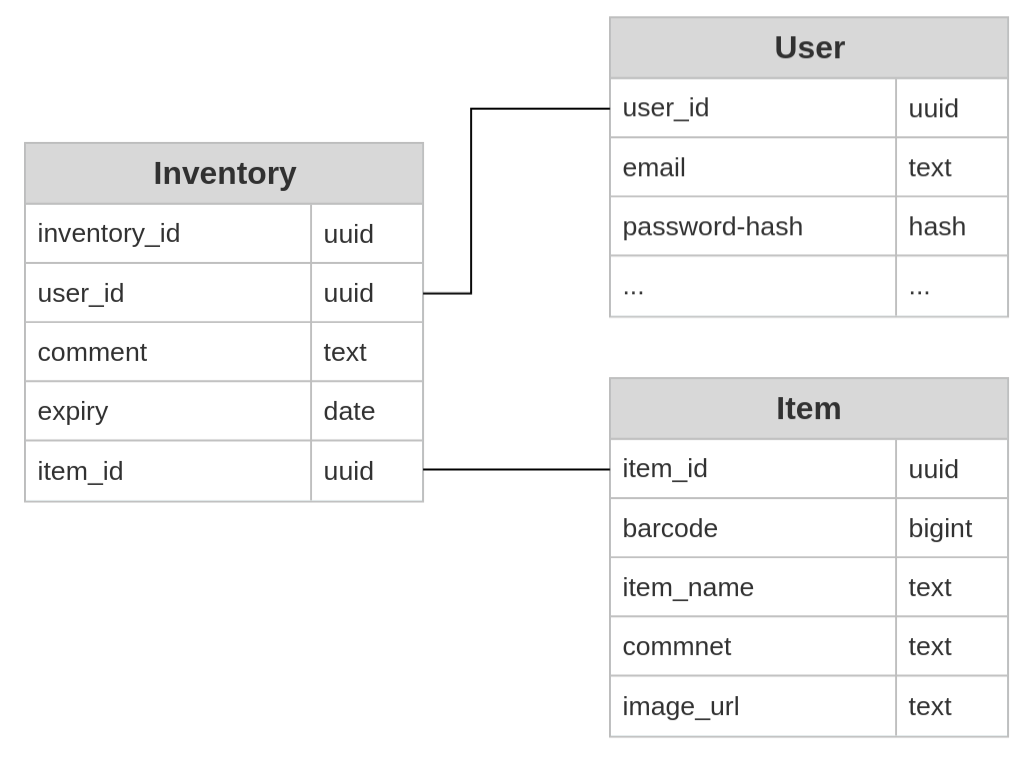
\includegraphics[width=1\textwidth]{Chapter 3/alexandre/db.png}
    \caption{DB Diagram}
    \label{fig:DB_Diagram}
\end{figure} 

Using Supabase made our database easy to set up and use, and the API provided both in JavaScript and python made interaction simple for both the Smart Fridge itself as well as the website and app.
However one disadvantage of Supabase is the lack of hosting for our Front Ends, meaning that we need to host them separately.
This aside, the back end worked exactly as intended and provided a secure location to transmit data to.

\subsection{App [ASH]}

Smartphones are owned by over 80\% \cite{stat} of all UK adults and with that apps have become the way people interact with many facets of modern life.
This why we decided to also allow the user to access the Smart Fridge via an app, along side the website, both of these services provide the user with the inventory of their Fridge and feed into APIs to provide insights.
While much of the core functionality overlaps with a website, the app needs to be designed very differently to work on a smartphone however the medium also provides opportunities such as sending notification the user as well as having a camera connected directly to the device.
With this in mind we planned to create an app that had all the core functionality of the website of viewing the inventory, making updates to the inventory, seeing insights about the inventory such as recipe recommendations and nutritional data and as well as dealing with user authentication.
The app will also expand on this by providing notifications based on expires, informing the user when the fridge is left open, and allowing the user to use their phone camera to scan in them when the Smart Fridge misses them.

React Native, Meta's mobile app development platform using the extremely popular React JavaScript user interface framework, was our natural choice for an app.
This is because React Native is used to create mobile apps for countless companies, ranging from Fortune 500s and start-ups \cite{react}, meaning it powerful and versatile enough to create anything we require.
Having prior experience in React also reduced the learning curve required to make this app.
Furthermore, as React Native is based on React, often used to create websites, code between the app and website could have been shared.
Eventually however, the decision was made to have the website written in python, regardless React Native can still render as a website meaning we also have an alternative website.

The core functionality of the app is is mostly supported by two external systems, the Supabase library that allows for quick and easy connection to our back-end and the Edamam API.
The Supabase library allows us easily create a connection to the database, allowing to to handle user logins and database looks-ups and updates.
There is also functionality to subscribe to events on the database, meaning the app will update without needing a manual refresh when and item is added to the Fridge.
Login also supports the “oauth” standard, allowing users to connect using a long list of accounts such as their Google or Facebook login, however this was disabled for the prototype as we only used dummy accounts with passwords.
The Edaman API provides the nutritional analysis and recipe search functionality of the app.
The API is very powerful and claims to contain the nutritional data of close to 900,000 foods and to have over 2.3 million recipes \cite{edman}.
More information about the API is in the section covering the website.
This along side the natural language processing on their end allows us to send over a list of the user items, as well as attached comments containing further information about the item such as brand or unit, and receive high quality data as a response.
These response can then be displayed to the user.

The Smart Fridge app consists of three primary screen, pictured below in figure \ref{fig:app}.

\begin{figure}[H]
    \begin{subfigure}{.33\textwidth}
      \centering
      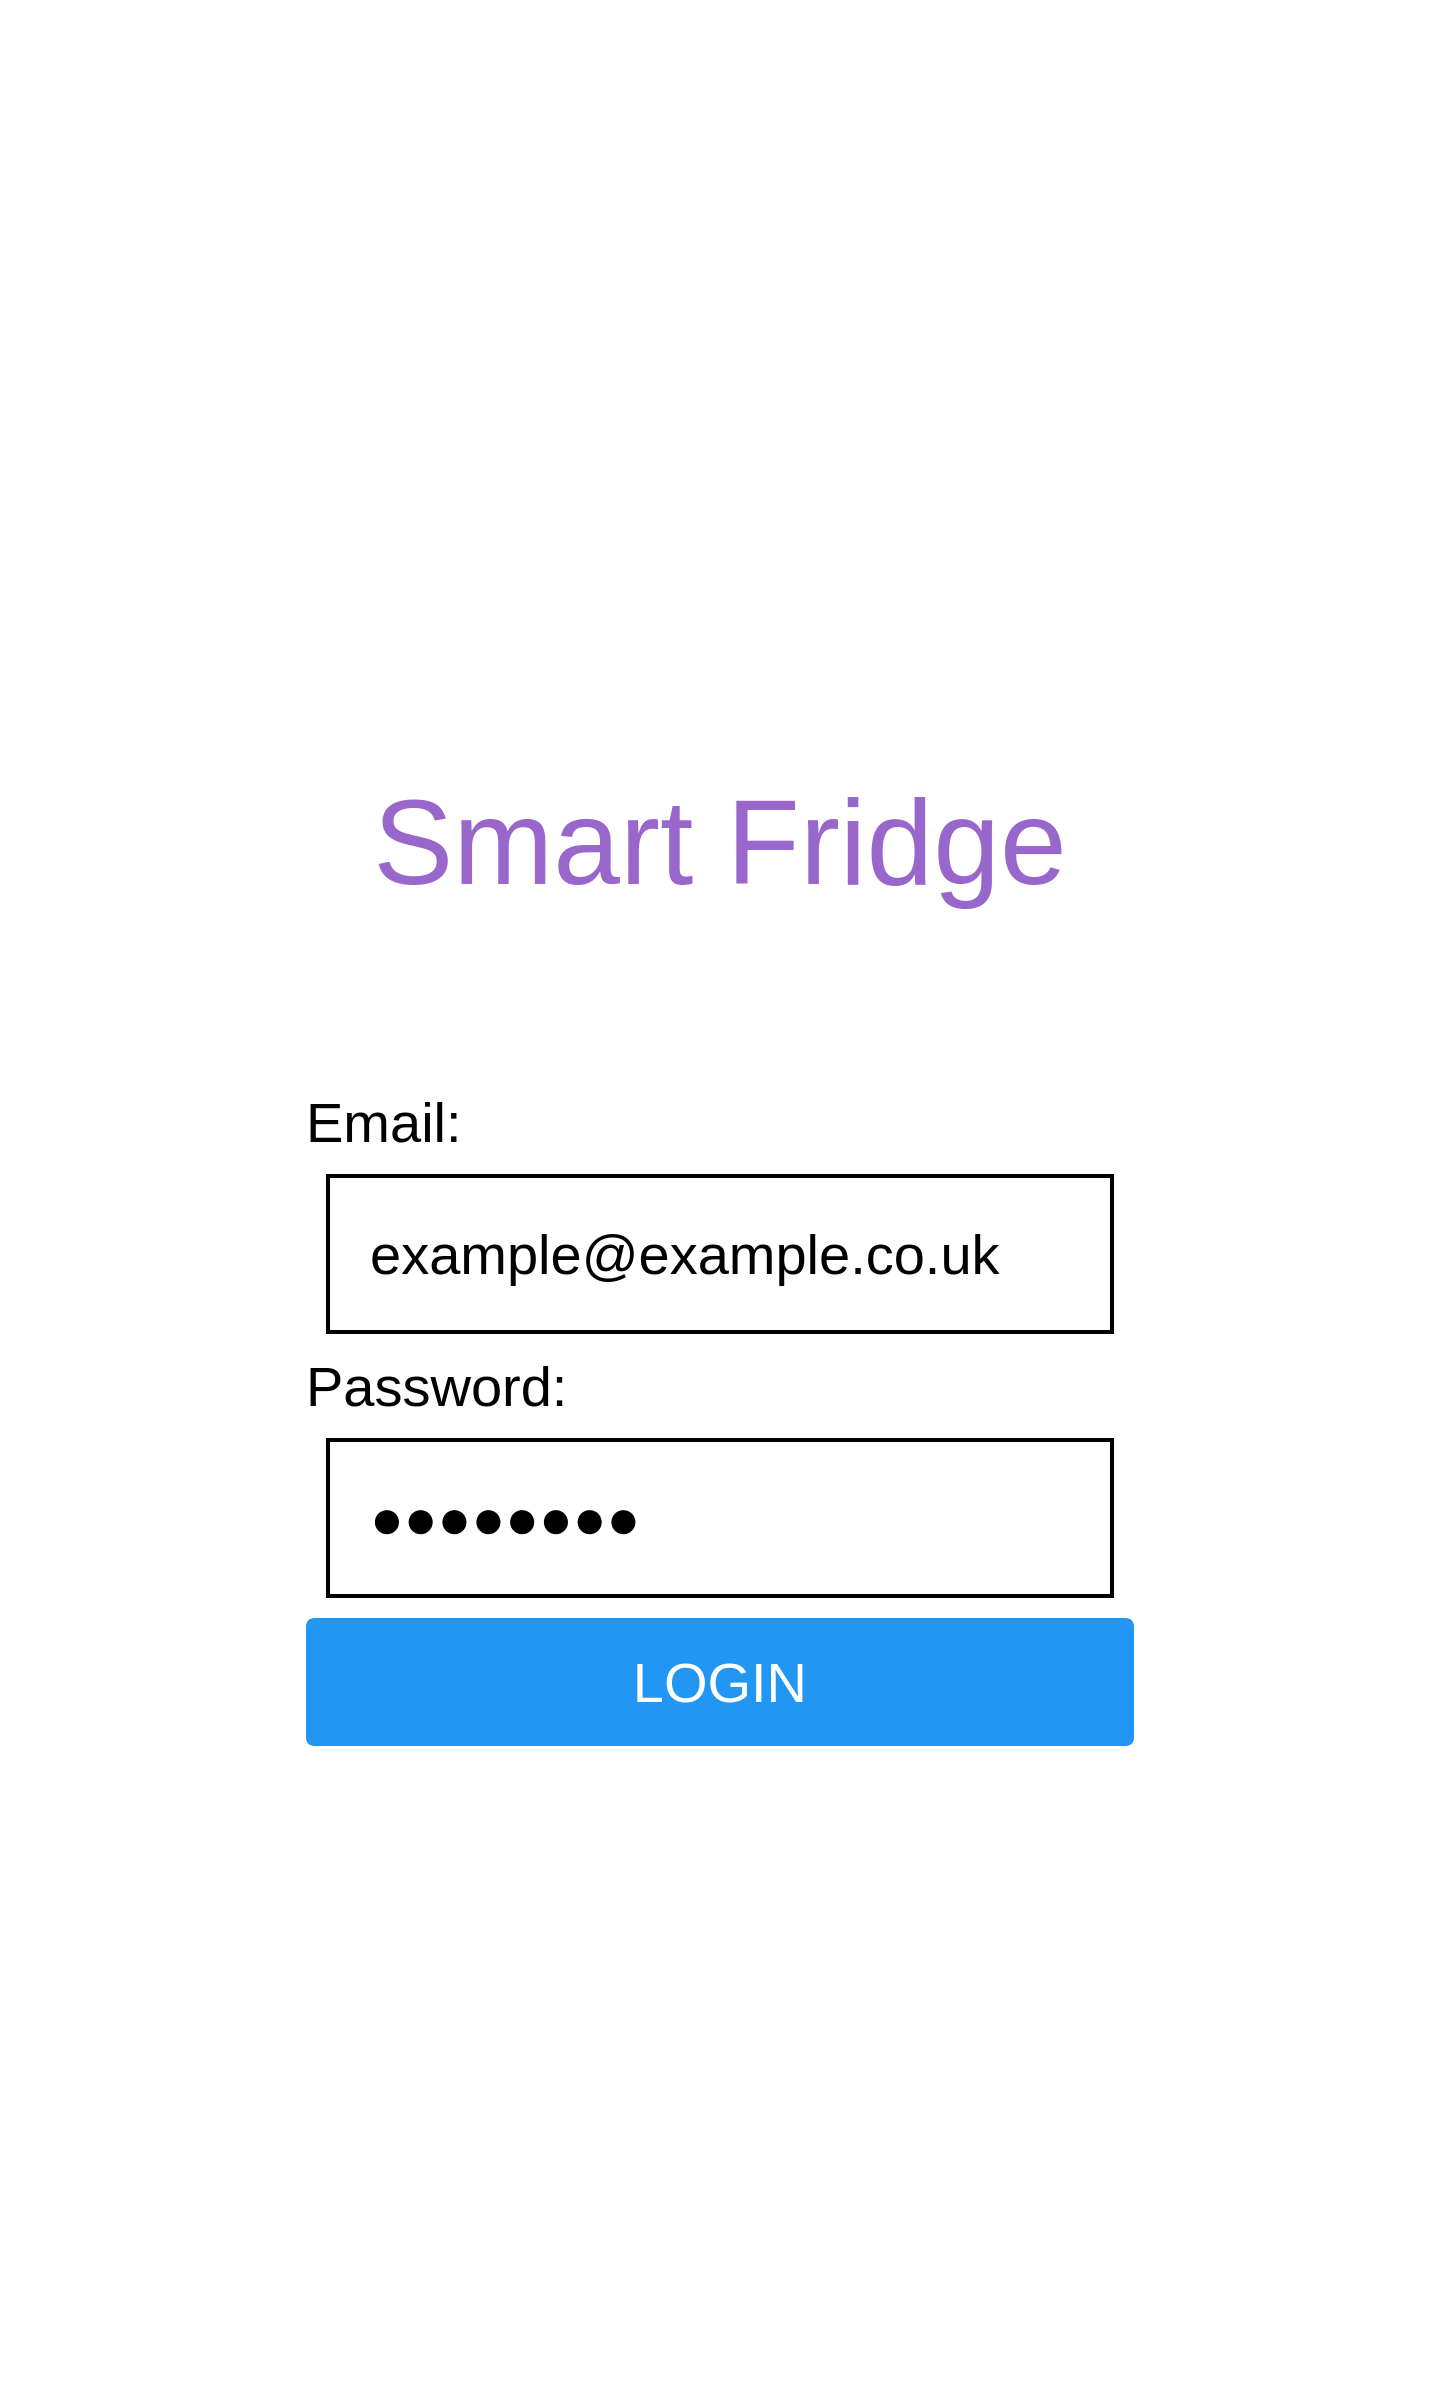
\includegraphics[width=.8\linewidth]{Chapter 4/app_pic/Login.png}
    \end{subfigure}%
    \begin{subfigure}{.33\textwidth}
      \centering
      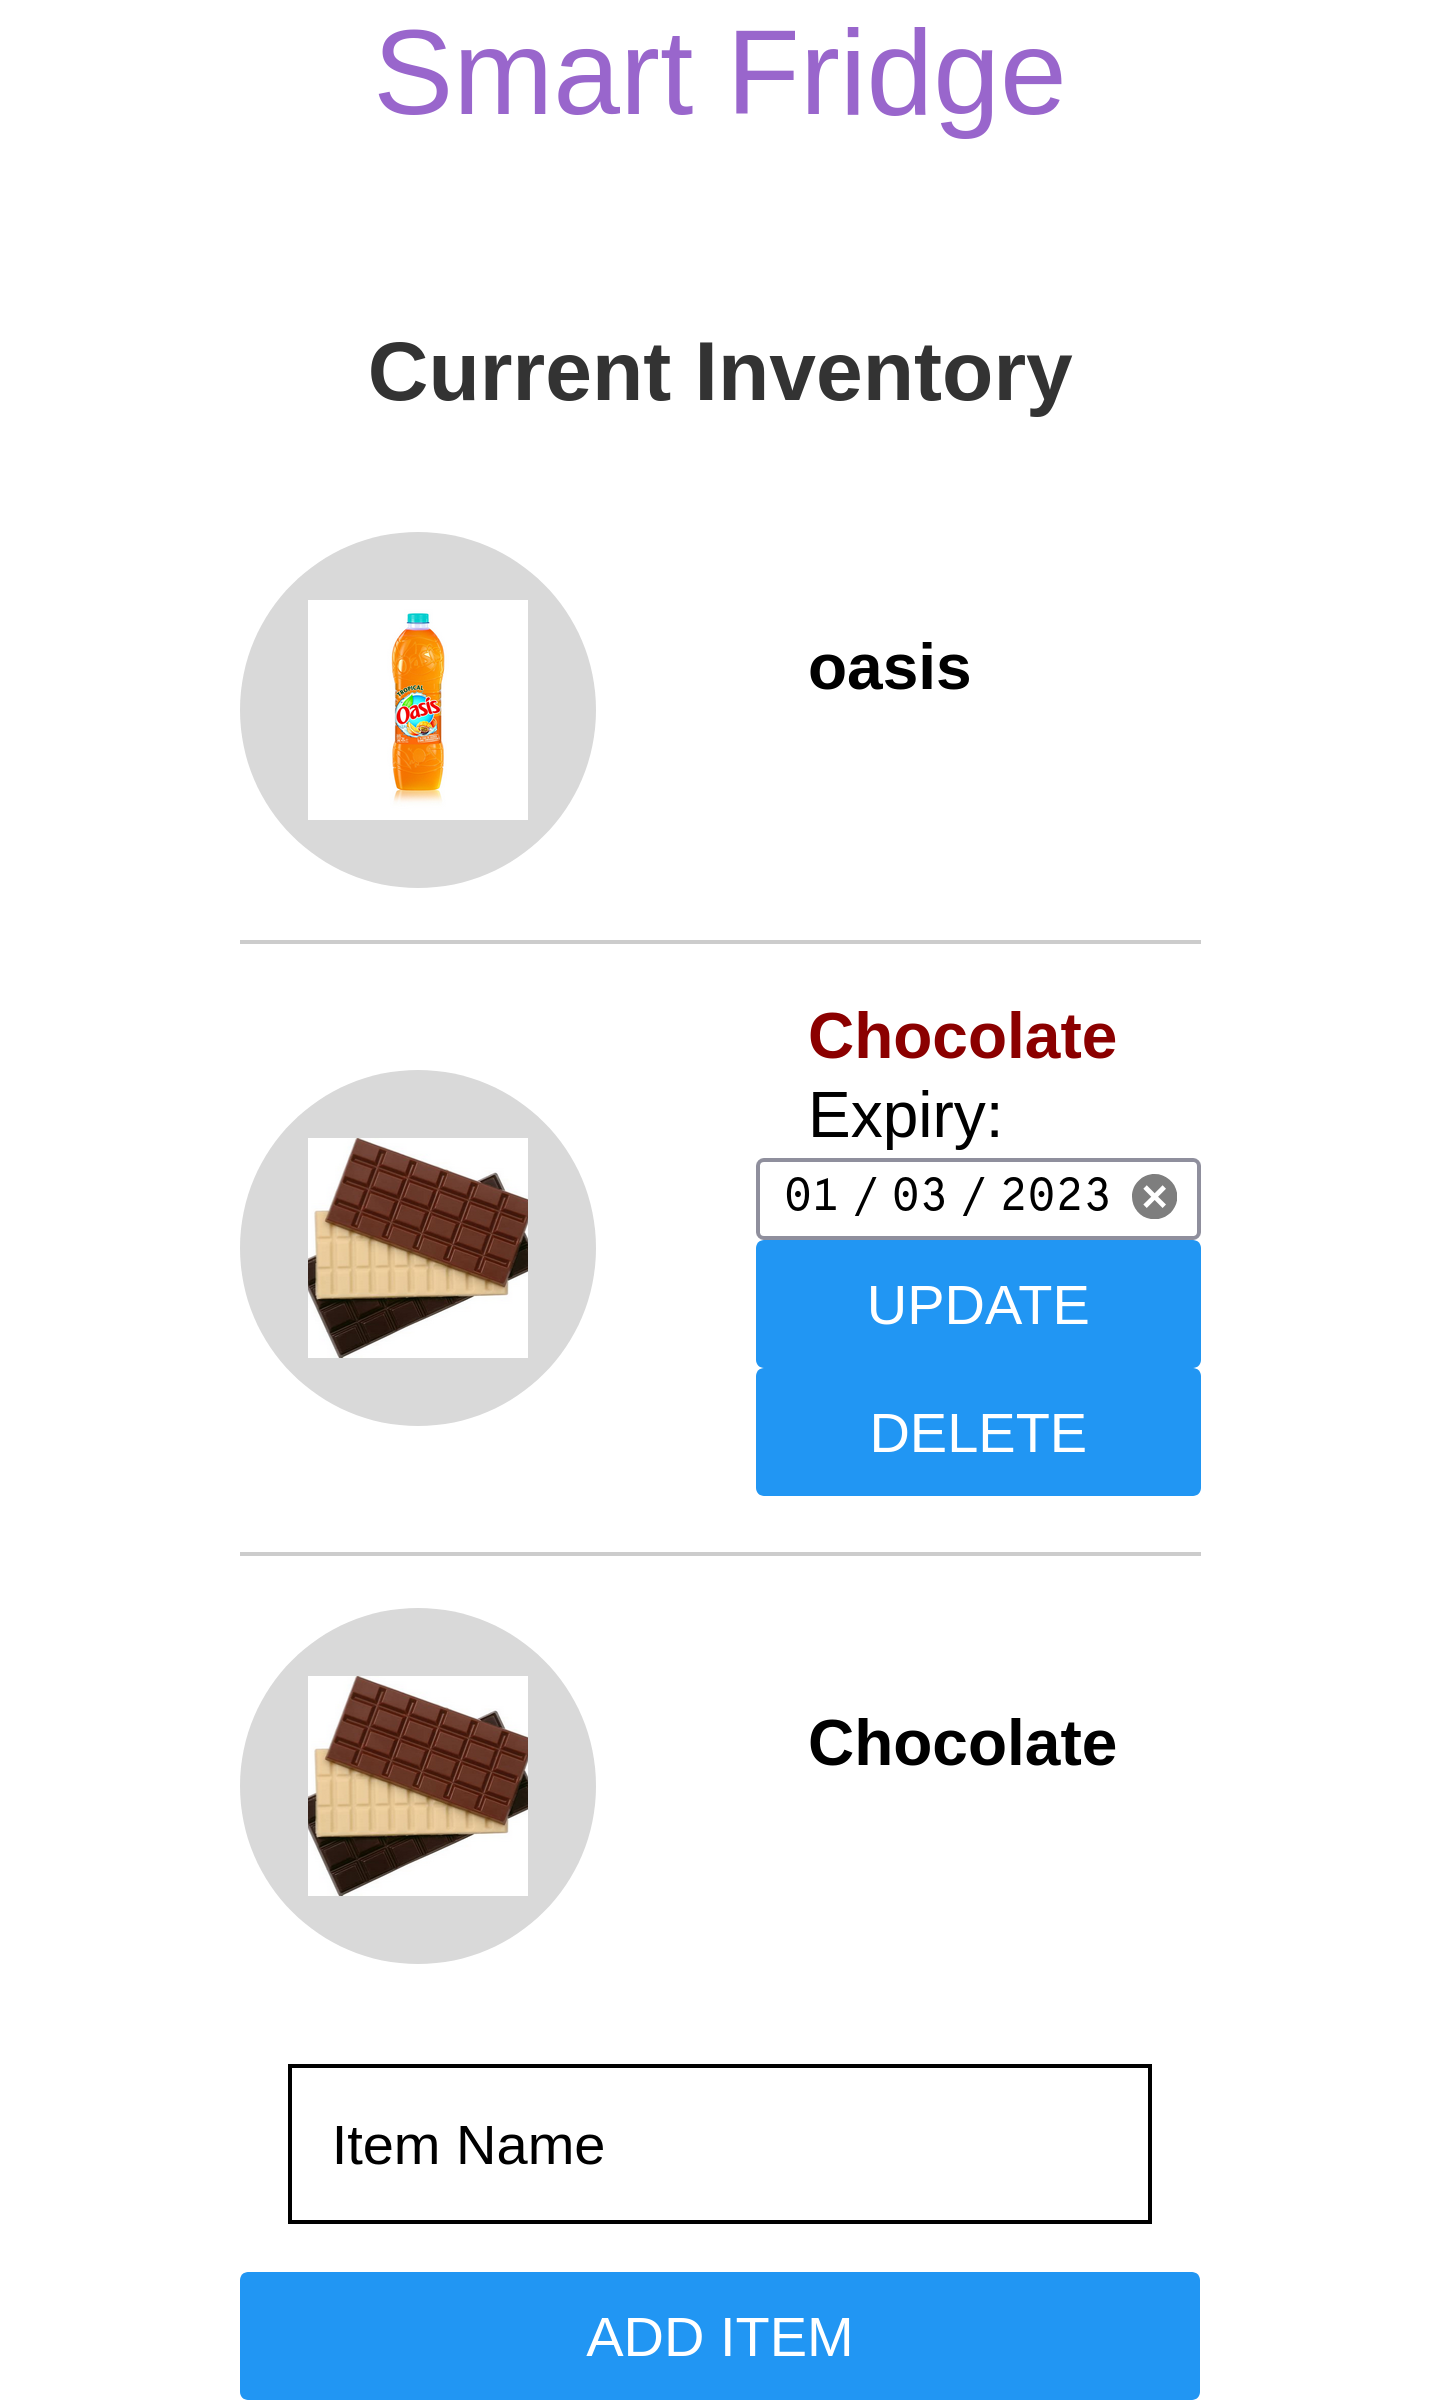
\includegraphics[width=.8\linewidth]{Chapter 4/app_pic/Inv.png}
    \end{subfigure}
    \begin{subfigure}{.33\textwidth}
        \centering
        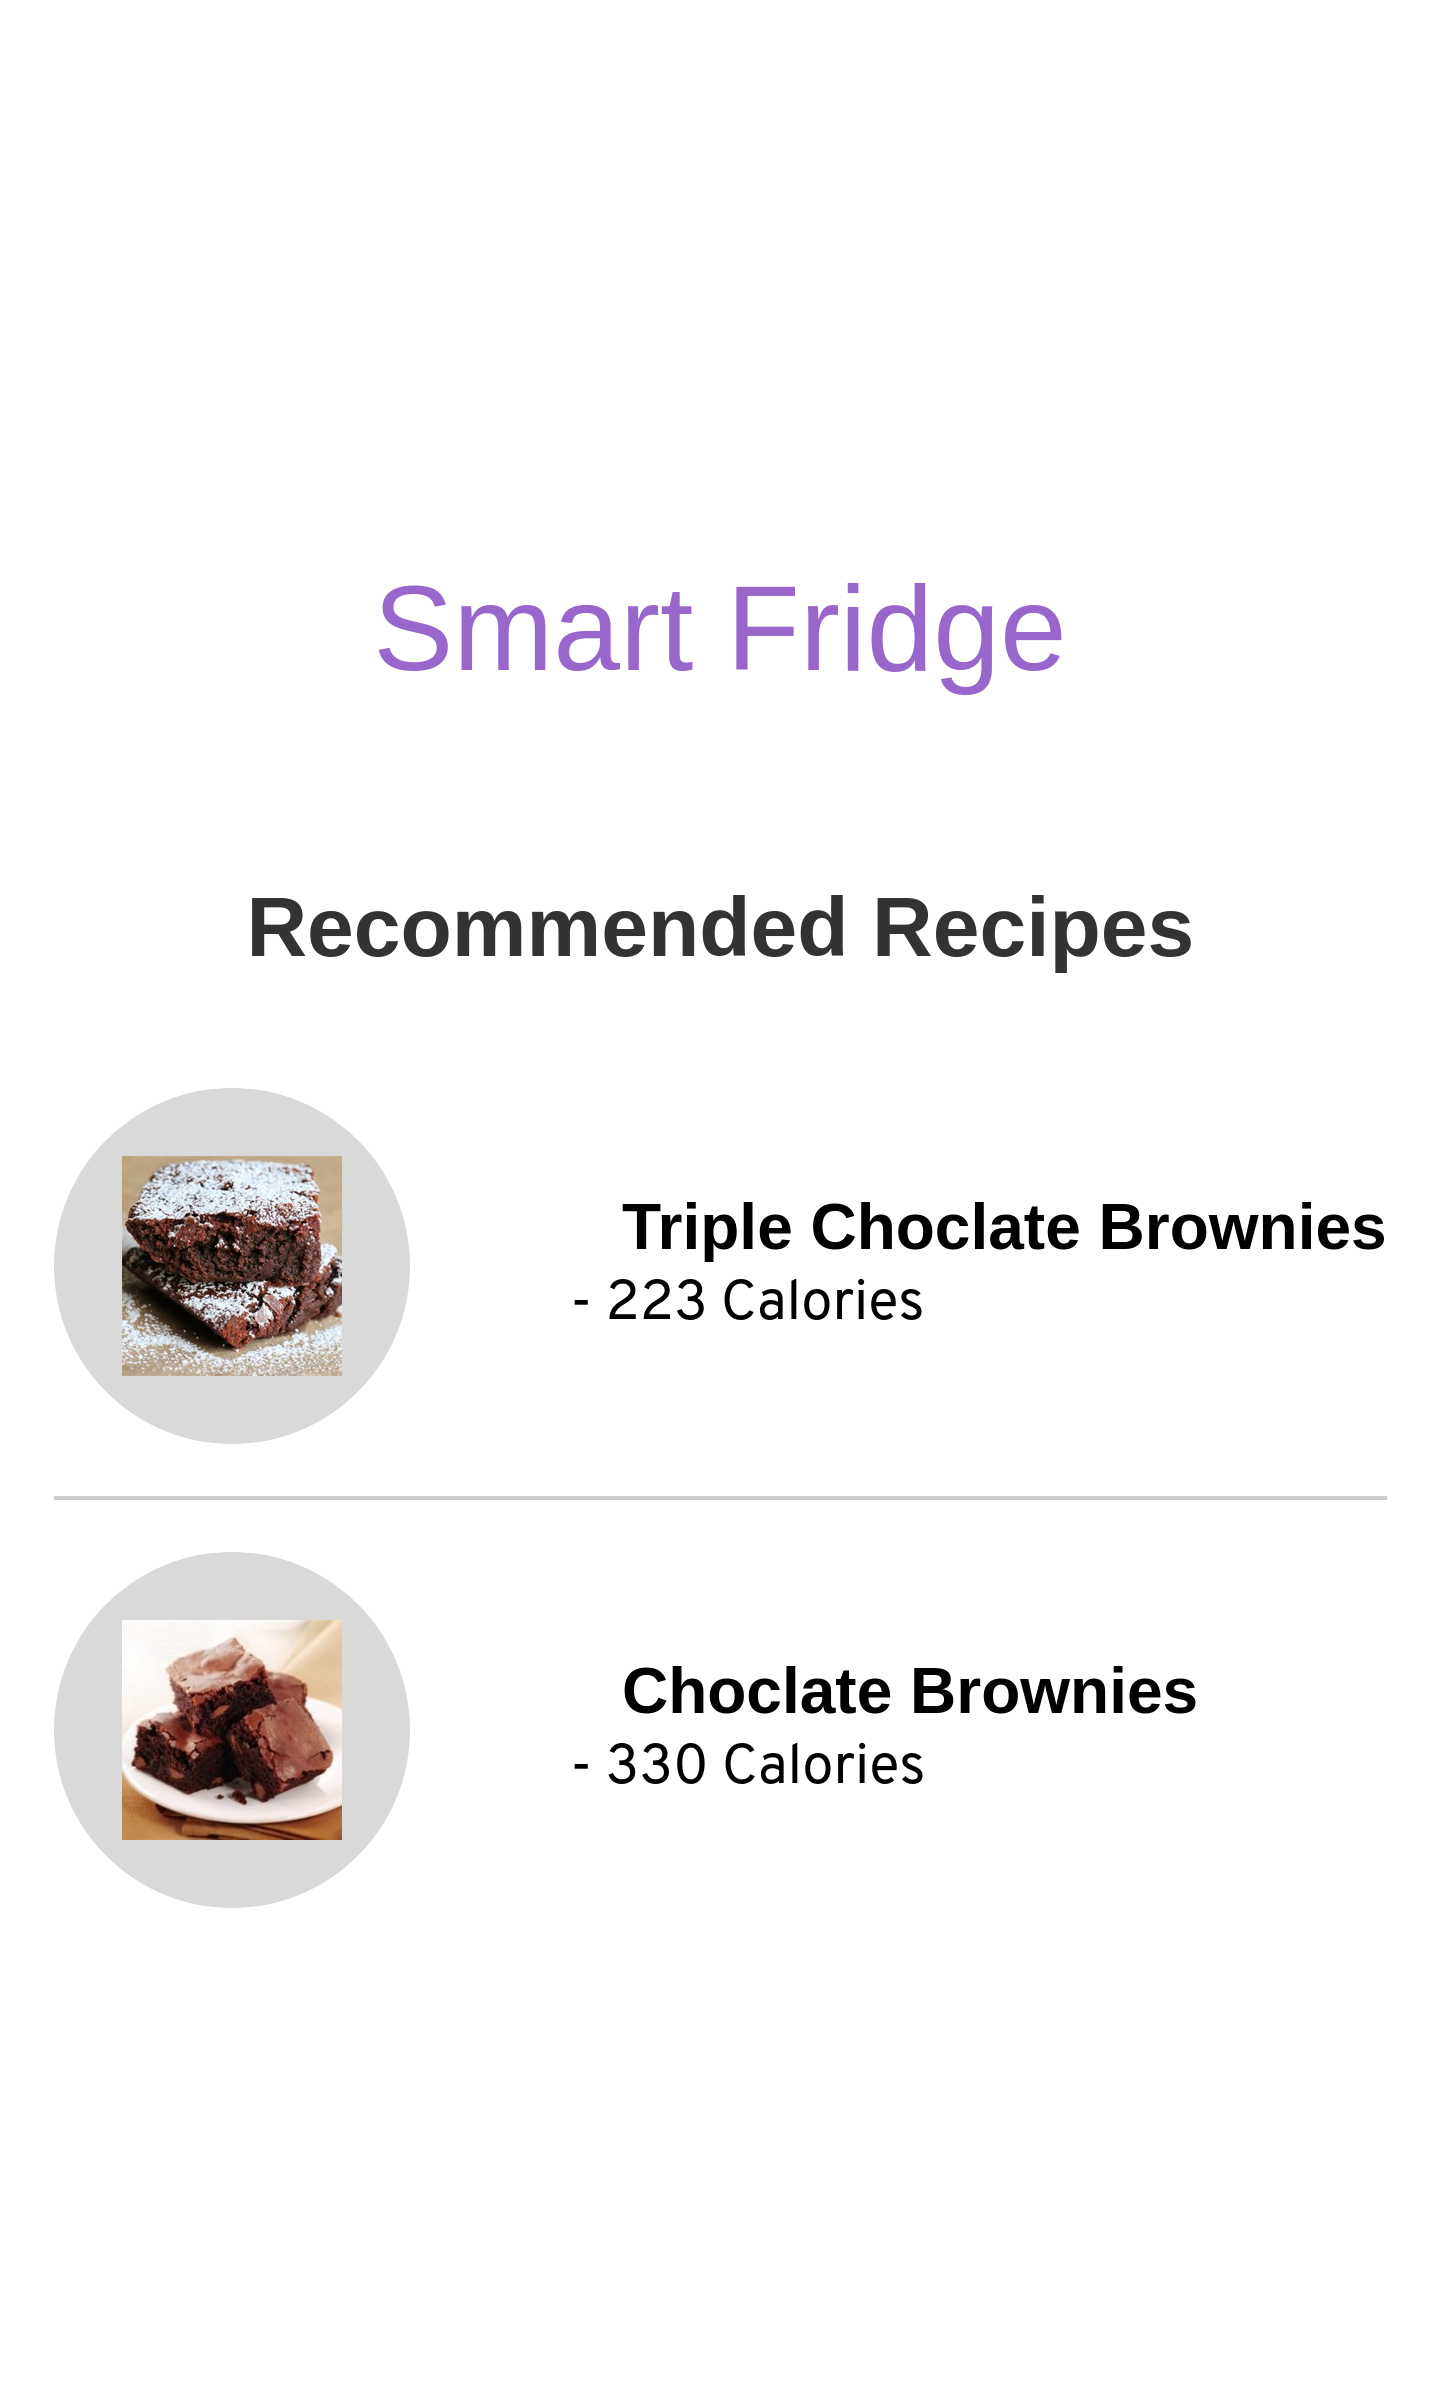
\includegraphics[width=.8\linewidth]{Chapter 4/app_pic/Rec.png}
    \end{subfigure}
    \caption{Screenshots of App.
Left to Right: Login, inventory, Recipes}
    \label{fig:app}
\end{figure}

The left image shows the Login-In screen, pictured filled with our dummy login details, where the user has to enter their username and password to login and gain access.
This will only have to be done once, as the login will then stores unless the user clears their App data.
The middle shows the primary inventory screen, this is the main screen where the user can view the inventory, seeing the name and expiry date of each of their items as well as a little picture provided by us to represent the item.
They can also manage the inventory, if need be, either by tapping an item to modify the expiry date or remove item.
The button below can be used to add an item by name.
The right image contains the recipe screen presenting the recipes from the API to the user, this screen can be reached by swiping right on the inventory and refreshed by pulling down.
To access a website the user simply clicks anywhere on the entry.

Testing the core functionality of the app was done throughout development, as a “Minimum Viable Product” approach was taken.
Meaning that the app began as a very bare-bone, but fully functional product which only showed the inventory.
By slowing adding to this base, and constantly testing the core feature, we were able to create a more complicated app whose core features had been thoroughly tested by the end of this initial development.
The app could have been improved with more solid test cases, simply to ensure every case was tested consistently.
However even without this method the end result meets all the set out goals and the app serves as a useful way for the user to view the collected data.

\subsection{Website [HH]}

The website  for the smart fridge was created to serve as a resource for managing the fridge inventory and searching for recipes.
It was built in Python using the Streamlit framework.
The Edamam API was utilised for its extensive database of quality recipes with a thorough nutritional breakdown.

The inventory data is hosted on Supabase, a cloud database service that provides an interface to access and manage data from external applications.
Supabase offers client libraries for several languages, including Python the language of the Smart Fridge website.

\subsubsection{User Login [HH]}

Upon visiting the website, users are prompted to log in or create a new account.
When the correct details are entered, the user can access the main page - the Smart Fridge.
Users remain logged in even after leaving the website thanks to a persistent web cookie.
Passwords are hashed before being stored to protect against unauthorized access.
Users can log out at any time by clicking the "Logout" button in the sidebar.
New accounts can be created by opening an expander.
Session states are used to temporarily store sensitive data that is required while the website is running.


\begin{figure}[H]
    \begin{subfigure}{.5\textwidth}
        \centering
        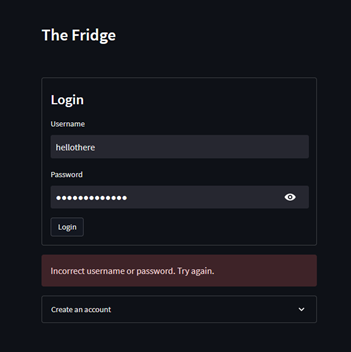
\includegraphics[width=.66\textwidth]{Chapter 4/Hamzah Website/UserLogin/Fig1.png}
        \caption{Demonstration of Login page showing error response}
    \end{subfigure}%
    \begin{subfigure}{.5\textwidth}
        \centering
        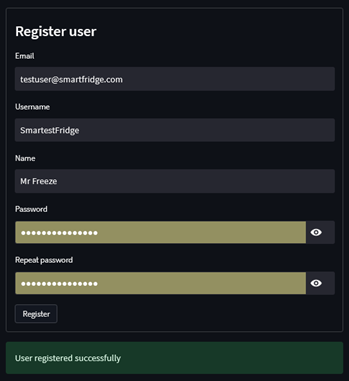
\includegraphics[width=.66\textwidth]{Chapter 4/Hamzah Website/UserLogin/Fig2.png}
        \caption{Registration demonstration}
    \end{subfigure}
    \caption{Login Screens}
\end{figure}

\subsubsection{Home Page [HH]}

The main page displays the user's inventory with useful options below.
The sidebar can be opened by clicking the arrow in the top left corner, where users can log out and access settings.

\begin{figure}[H]
    \begin{subfigure}{.5\textwidth}
        \centering
        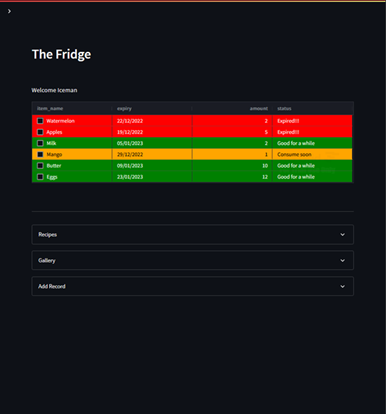
\includegraphics[width=.66\textwidth]{Chapter 4/Hamzah Website/HomePage/Fig3.png}
        \caption{The main page showcasing the inventory}
    \end{subfigure}%
    \begin{subfigure}{.5\textwidth}
        \centering
        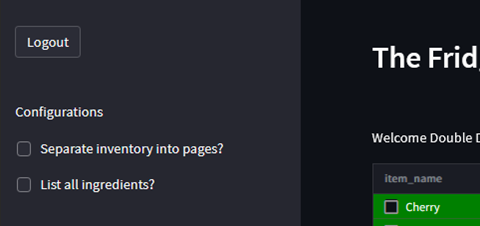
\includegraphics[width=.66\textwidth]{Chapter 4/Hamzah Website/HomePage/Fig4.png}
        \caption{The sidebar options}
    \end{subfigure}
    \caption{Home Page}
\end{figure}

\subsubsection{Fetching Data [HH]}

The website connects to the database using the Supabase client library and authenticates the connection with a URL and key.
SQL statements are used to retrieve and modify data stored in the database.
To retrieve the inventory data, an SQL select statement is used to specify the columns to show to the user, with a condition to only access data that belongs to the current user.

\begin{figure}[H]        
    \centering
    
\includegraphics[width=1\textwidth]{Chapter 4/Hamzah Website/FetchingData/Fig5.png}
    \caption{SQL statement to retrieve the fridge inventory from Supabase}
\end{figure} 

\subsubsection{Inventory table [HH]}

To display the inventory, we chose to use a table.
Tables are readable and suited for displaying large data sets.

\begin{figure}[H]        
    \centering
    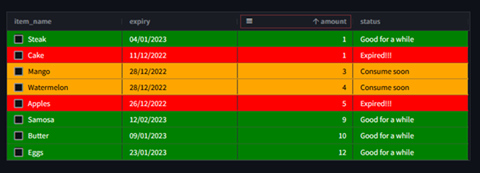
\includegraphics[width=.66\textwidth]{Chapter 4/Hamzah Website/InventoryTable/Fig6.png}
    \caption{Inventory sorted by quantity}
\end{figure} 

The table includes columns for the item name, expiration date, quantity, and status of each item in the inventory.
These columns were chosen because they convey the most relevant and useful information to the user.
Each row is highlighted in a colour corresponding to their expiration status.
Green is for food that is good for a while, orange if only a few days remain until expiration, and red for expired food items that should be handled with caution.

The table can be sorted by clicking on any column, which allows users to easily find specific items or view their inventory in different ways.
For example, they could sort by expiration date to see which items need to be used up first.

In addition to sorting, the table allows users to rearrange columns by dragging them to a new position or hide columns by dragging them outside of the table.
Users can also filter values in a column by clicking on the hamburger icon that appears when hovering over a column.

\begin{figure}[H]        
    \centering
    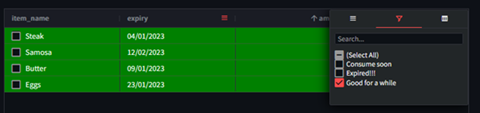
\includegraphics[width=.66\textwidth]{Chapter 4/Hamzah Website/InventoryTable/Fig7.png}
    \caption{Filtering option inside the hamburger menu}
\end{figure} 

An option to paginate the table exists in the sidebar.
Pagination separates rows into different pages to make it easier to navigate.
This is especially useful when the inventory contains a large number of items.

\begin{figure}[H]        
    \centering
    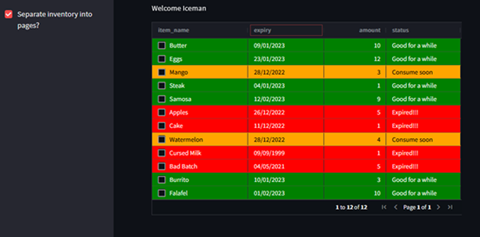
\includegraphics[width=.66\textwidth]{Chapter 4/Hamzah Website/InventoryTable/Fig8.png}
    \caption{Pagination option}
\end{figure} 

The data from Supabase was stored using the Pandas DataFrame and presented using an AgGrid.
The DataFrame is a flexible and mutable two-dimensional table, while the grid was designed to be used in web applications.
The AgGrid JavaScript-based grid type that has useful applications such as allowing us to execute useful commands (such as JavaScript code), but is not as flexible within Python.
Using Pandas alongside the AgGrid grants access to the useful qualities of both.

Since the expiration status is not stored in the database, the website must be able to determine it based on known information.
I created a function which returns the difference in days between an input date and the current day.
The parser function can extract a date from a string containing a date in a many different formats, (such as the different regional date formats like, or different delimiters such as '/' and '-').This is also done for the today date to prevent a ValueError exception that would occur if the expiration date was in a different format to the standard 'datetime' format'.

\begin{figure}[H]        
    \centering
    \includegraphics[width=.66\textwidth]{Chapter 4/Hamzah Website/HowItWasCoded/fig9.png}
    \caption{Function that calculates the difference in days, regardless of format}
\end{figure} 

For each date in the table, the difference in days was calculated and stored in a list.
If the difference in days is negative, then it indicates that the food is already expired.
Otherwise, the food is still safe to eat.
Based on the comparisons shown in \ref{fig:awefulcode}, the specified string of text is stored in a new column of the table, reflecting the status of each item.


\begin{figure}[H]
    \begin{subfigure}{.5\textwidth}
        \centering
        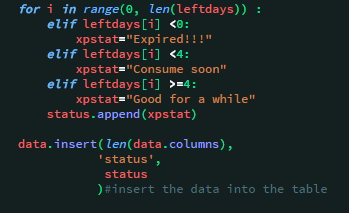
\includegraphics[width=.66\textwidth]{Chapter 4/Hamzah Website/HowItWasCoded/fig10.png}
        \caption{Code that evaluates expiration status and inserts it to the table.}
        \label{fig:awefulcode}
    \end{subfigure}%
    \begin{subfigure}{.5\textwidth}
        \centering
        \includegraphics[width=.66\textwidth]{Chapter 4/Hamzah Website/HowItWasCoded/fig11.png}
        \caption{JavaScript code that changes appearance of a grid based on expiration evaluation, and code that creates and configures the grid.}
        \label{fig:badcode}
    \end{subfigure}
    \caption{Code Snippets}
\end{figure}

The grid configurations are set before it is displayed.

In Fig \ref{fig:badcode} Line 203 to 224 shows the JavaScript code (JsCode) used to modify the colour of the grid.
The status column on the grid will contain one of the three conditional values, and so will be red, orange or green depending on its expiration status.

To execute the JsCode, we must use an AgGrid.
As we transfer the data from the DataFrame to the grid, we also configure the grid to use checkboxes (facilitating record deletion) and allow JsCode.

Line 228 allows the grid to be edited by clicking a cell and typing on a keyboard.
This showcases a potential method to directly edit the values to the database.

\subsubsection{Adding Records [HH]}

To add new items to the inventory, users can enter the name, expiration date, and quantity in the "Add Record" tab.
The expiration date can be chosen from a calendar input widget or entered manually.

\begin{figure}[H]        
    \centering
    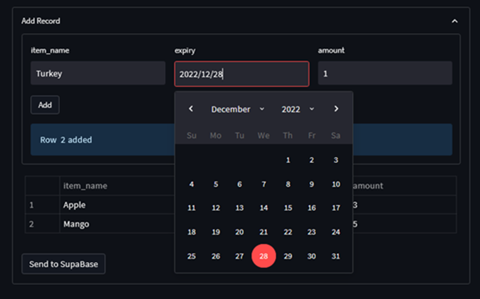
\includegraphics[width=.66\textwidth]{Chapter 4/Hamzah Website/AddingRecords/Fig12.png}
    \caption{Interface to add new items to the database}
\end{figure} 

Calendar widget used for date entry.

When the "Send to SupaBase" button is clicked, the data in the table is converted into a list of dictionaries.
This format allows multiple items to be inserted correctly using an SQL insert statement.
The inventory table is then automatically updated, and the "Add Record" table is reset for adding more items.

Three columns for data input are created, based on the Pandas DataFrame existing in the session state.
An array stores the inputs until the records are submitted.

When new records are sent to the Supabase, they must be assigned a username key, otherwise it will not be recognised to be part of the current user's inventory.
Since the DataFrame already needs to be converted into a list of dictionaries , adding a new key and value is simple.
Now the data can be inserted into the database with the SQL insert statement on line 567.

\begin{figure}[H]
    \begin{subfigure}{.5\textwidth}
        \centering
        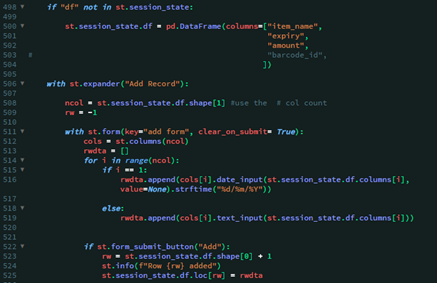
\includegraphics[width=.66\textwidth]{Chapter 4/Hamzah Website/AddingRecords/Fig13.png}
        \caption{Code for creating and accepting data inputs}
    \end{subfigure}%
    \begin{subfigure}{.5\textwidth}
        \centering
        \includegraphics[width=.66\textwidth]{Chapter 4/Hamzah Website/AddingRecords/Fig14.png}
        \caption{Code designated the ownership of new items to the user that added them}
    \end{subfigure}
    \caption{Code Snippets 2}
\end{figure}


\subsubsection{Deleting Records [HH]}

To delete items from the inventory, users can select multiple items using the checkboxes and confirm deletion with a prompt.
The selected items are then removed from the database using an SQL delete statement.



\begin{figure}[H]        
    \centering
    \includegraphics[width=.66\textwidth]{Chapter 4/Hamzah Website/AddingRecords/Fig12.png}
    \caption{Demonstration of how items are deleted from the table using checkboxes}
\end{figure} 

When the grid was configured, I created a response that returns the values selected by the user.
I programmed the 'Delete' button to appear only if items are selected.
When clicked, the grid is converted into a list, and processed into an SQL statement which deletes item with the matching details.

The 'in' method allows a list to be specified.

\begin{figure}[H]        
    \centering
    \includegraphics[width=.66\textwidth]{Chapter 4/Hamzah Website/AddingRecords/Fig12.png}
    \caption{Converting selected items into a suitable format for SQL deletion}
\end{figure} 

\subsubsection{Searching for Recipes [HH]}

Recipes can be found based on items in the fridge.
Recipes can also be filtered based on dietary requirements such as Kosher, low-sugar and vegan, or by the calories per serving.
Drop down menus are used to select the ingredients and dietary requirements.
The nutritional options (calories, carbohydrates and sugar) can be specified by keyboard input or the positive and negative buttons on the box.
The  value can be left at 0 if the user does not wish to specify a requirement.

\begin{figure}[H]
    \begin{subfigure}{.5\textwidth}
        \centering
        \includegraphics[width=.66\textwidth]{Chapter 4/Hamzah Website/SearchingForRecipes/Fig17.png}
        \caption{Fig demonstrating the recipe interface with generated recipes showing nutritional information}
    \end{subfigure}%
    \begin{subfigure}{.5\textwidth}
        \centering
        \includegraphics[width=.66\textwidth]{Chapter 4/Hamzah Website/SearchingForRecipes/Fig18.png}
        \caption{Recipes with the ingredients listed}
    \end{subfigure}
    \caption{Recipe Display}
\end{figure}

After the search button has been clicked, the Edamam API returns the available recipes.
If there are no available recipes, then the website will prompt the user to reconsider the search parameters.

For each recipe, a link to the original website is displayed, along with additional data such as nutritional information based on servings, preparation time, and the ingredients needed for the recipe.
For a more compact view, the recipe list can be disabled from the sidebar.

A URL is used to interact with the Edamam API.
It is composed of an application ID and key (received when signing up), ingredients, and optional parameters such as dietary requirements.

\begin{figure}[H]        
    \centering
    \includegraphics[width=.66\textwidth]{Chapter 4/Hamzah Website/SearchingForRecipes/Fig19.png}
    \caption{the URL format accepted by Edamam API}
\end{figure} 

When the user selects their choice of ingredients and dietary requirements, they are stored in a list.

Ingredients and dietary requirements are formatted slightly differently in the Edamam URL.
In both cases, the 'join' function concatenates each element of the list with the string specified in inverted commas.

The API returns recipe data in the JSON format which is convenient to parse.
At this point, the recipes are evaluated against the nutritional conditions set by the user.
The recipes that meet the criteria, they are displayed with the aforementioned information.

\begin{figure}[H]
    \begin{subfigure}{.5\textwidth}
        \centering
        \includegraphics[width=.66\textwidth]{Chapter 4/Hamzah Website/SearchingForRecipes/Fig20.png}
        \caption{Code showing how the user choices are formatted into an Edamam query.}
    \end{subfigure}%
    \begin{subfigure}{.5\textwidth}
        \centering
        \includegraphics[width=.66\textwidth]{Chapter 4/Hamzah Website/SearchingForRecipes/Fig21.png}
        \caption{Code showing how the JSON data received by Edamam API is processed and displayed to the user.}
    \end{subfigure}
    \caption{Code Snippets 3}
\end{figure}

\subsubsection{Developments [HH]}

My first prototype started with reading a CSV file and displaying them on the screen.
The aim of this was to demonstrate how data could be displayed.
The CSV file was read and parsed into a DataFrame.
It was imperative to use a cloud-hosted database solution, so the website soon transitioned over.

When I first used the Supabase library to insert the items, the result were less than ideal: the items were added as a 'dictionary' and were all contained in one cell.

I then switched to another SQL module in python, known as Psycopg2.
I was able to insert items correctly.
I extracted the values from the Dataframe, concatenated them into a single string and then inserted them into the database.
Psycopg2 uses a 'server cursor' which is an “object that enables traversal over the rows of a result set”.

While it was an effective solution, there was a caveat.
An additional database password would have to be created and stored somewhere; without a password Psycopg2 is unable to connect.
This is not inherently a big issue, but since we executed other SQL statements with the Supabase client library, it made sense to use it where possible.

By examining the Pandas documentation \cite{pd}, I discovered some useful data manipulation functions.
The DataFrame could be converted into a dictionary using the function 'pandas.DataFrame.to\_dict('records)'.
If multiple items exist in the DataFrame it is converted into a list of dictionaries.
 In the list, each dictionary represents a single record.
The keys in the dictionaries corresponds to the column names in the database, and the values represent the data to be inserted for each column.
This method worked perfectly with the Supabase library.
Inserting the items this way ensured that each item and their respective details were contained in the correct place.

\section{Enclosure}
\subsection{Prototype 1 [JG]}

The fridge has become an essential product in almost any kitchen since its invention.
As a result, the main ideas behind its design have been refined to a point of near perfection, leaving little room for innovation, and even less for improvement.
Therefore, the challenge when designing the Smart Fridge did not come from trying to change or improve an established design, but rather came from implementing new features whilst staying as close to this design as possible.

The Smart Fridge would take the form of a box which would be large enough to fit a small bottle of milk inside.
The ESP camera was to be fitted into the door.
Initially, it was decided that the door would be thick and hollow to store the camera and the electrical components associated with it.
The door would also house the Hall effect sensor to detect whether the fridge door was open.
The weight sensor was then to be placed on the bottom of the fridge, with a plate above it on which items would be placed.
The remaining electrical components would then be placed in this gap.
For the prototype it was decided that this would remain open for easier access should any changes need to be made.
The CAD design for this is shown below with dimensions.

\begin{figure}[H]        
    \centering
    \includegraphics[width=.33\textwidth]{Chapter 5/Box/BoxSchematic1.png}
    \caption{Initial design of Smart Fridge.}
    \label{fig:initaldesign}
\end{figure} 

The biggest issue with this design was its size.
The dimensions of the box were 300mmx300mmx400mm in addition to the door which was 300mmx25mmx400mm.
 Therefore, it is likely that this design would have required 4 sheets of acrylic to build which would have been too expensive.
As a result, a new design was proposed with a smaller size.
These changes along with the new dimensions are shown below.

\begin{figure}[H]        
    \centering
    \includegraphics[width=.33\textwidth]{Chapter 5/Box/BoxSchematic2.png}
    \caption{Updated Fridge Design.}
    \label{fig:updatedfridge}
\end{figure} 


In figure 2 the dimensions of the main box were all reduced by 100mm, with the relevant changes also being applied to the dimensions of the door.
Figure 2 also shows the change from the ESP camera to a webcam, which now protrudes significantly from the door.
The webcam also has a much larger cross-sectional area with a diameter of around 33mm.
Despite these changes, the design was still too big, so a new design was proposed.
This is shown below.

\begin{figure}[H]        
    \centering
    \includegraphics[width=.33\textwidth]{Chapter 5/Box/Schematic2DoorOpen.png}
    \caption{Fridge Design using 2 acrylic sheets.}
    \label{fig:fridge2sheet}
\end{figure} 

Figure 3 shows the changes made to the previous box design.
These changes reduced the required acrylic sheets from 3 to 2.
Firstly, the dimensions of the box were changed in order to achieve the maximum size possible while using no more than 2 acrylic sheets.
As a result, the dimensions of the base of the box were decreased, whilst the height was increased.
Previously it had been decided that the door would be a separate, thinner box.
However, to save acrylic, it was necessary for the door to be flat.
As a result, the components that would have previously been stored within the door now had to be stored under the weight sensor plate.
This meant that the weight sensor plate had to be raised by a few centimetres.
This box was then built with the final product shown below.

\begin{figure}[H]        
    \centering
    \includegraphics[width=.33\textwidth]{Chapter 5/Box/PictureOfBox1.png}
    \caption{First Built Box}
    \label{fig:firstbuilt}
\end{figure} 

There were several issues with the proposed design in figure 4.
The most noticeable of these issues is the collapsed weight sensor plate inside the box.
This happened as too much space was given on each side to ensure it would fit.
The other main problem with the box was that gluing objects onto acrylic was difficult.
This was especially true of the side plates and the door where objects had to be glued on vertically and would sometimes slide down.
This caused further problems with the hinges as they did not remain in their exact positions when stuck.
The hinges also did not allow the door to close entirely, leaving a small yet significant gap between the door and the box.
As a result, many aspects of the box had to be redesigned which led to a new proposal for the box design.
This is shown in the image below.

\begin{figure}[H]        
    \centering
    \includegraphics[width=.33\textwidth]{Chapter 5/Box/BoxDesign3.png}
    \caption{Fridge Design with no Hinges}
    \label{fig:designnohinges}
\end{figure} 

When designing the new box, shown in figure 5, the main idea was to remove the need for glue.
For the hinges, this was achieved by making a small hole in both the top and bottom plates of the box.
Then a single tooth was added onto the corresponding sides of the door to fit through these holes.
This also removed the need to use hinges which caused issues when closing the door in the previous design.
However, this meant that the door, now inside the box, would close in on itself.
To prevent this from happening, it was decided that small pieces of acrylic could be placed to act as door stoppers.
Each of these would be held in place by a single screw.
Additionally, the outward facing edge of the weight sensor plate had to be moved back into the fridge in order to avoid collisions with the door.
There was also a reduction in the height of the box as the previous design felt disproportionately tall.
Small changes were also made to the way in which the door handle was held in place.
In this design, holes were cut into the door for the two ends of the handle to be more securely attached.

\subsection{Prototype 2 [YJ]}

The box design for prototype 2 was the second iteration designed to make the box more user-friendly and fix the previous issues that prototype 1 encumbered.
However, facing concerns with a small budget, the containment would continue to use single-layer pieces of acrylic sheets.

The containment for the brains of the Smart-Fridge is below the main visible user body allowing easy access to the board by uncapping the bottom plate.
The magnets that detect when the door is open now mimic a soft closing door is a standard in most modern expensive fridges.
Magnets glued inside engravings allow for direct non-contact magnetic snapping to each other when the door is closed.
The plate onto which the Load cell and the Motherboard also use magnets to keep the platform intact.

The new design has no extra protrusions except for the camera.
There is simplistic cable management using zip ties.
The hinges from the first build-in prototype one secured through screws and nuts rather than glue resulting in a secure design as the hinges before were not firm and kept falling.
The redesign of the door handle resulted in curved edges rather than sharp which were previously not user-friendly and could have been harmful to the user.

\section{Reflections}
\subsection{Isaac Baglin [IB]}
My goal for this project was to develop skills in systems engineering.
To do this, I put myself on the microprocessor team so that I could plan, design, and integrate subsystems.
During the earlier weeks of the project, I helped plan the project by breaking the overall task into smaller subsystems.
It was also important that we discussed the dependencies between sections to make integration easier.
It was my personal responsibility to test the weight sensor, the buzzer and the esp32 camera module.
Within these tasks I selected the components, programmed them, and integrated them into the larger system.
This meant I was able to contribute both to hardware and software elements of the project.

The largest challenge that I faced was that the esp32 camera module didn't have a higher enough resolution to pick up barcodes in images.
This camera module was designed to take videos not isolated images therefore programming the module to take individual images was very challenging and time consuming.
Given the issue was a resolution problem, I had no choice but to scrap the module.
Thankfully, because of the planning in the earlier weeks of the project, we had a web camera available which could be used instead.
In future projects, more time should be taken to research the components and their feasibility.
The esp32 camera was chosen because it was pre-built on the microprocessor however because it wasn't designed to take individual images, the module shouldn't have been pursued to start with.
The time wasted on this module could have been spent adding additional features to the product or further assisting other group members with their sections.

Despite this one issue I feel as though I contributed greatly to the group's workload, I also acted as a valuable group member by being a key planner for the project by constantly contributing to the group discussions.
Given how dependent other subsystems were on the hardware, I made sure to meet all my personal deadlines as early as possible.
I was able to meet my personal objects of planning, designing, and integrating subsystems and the problems with the camera module allowed me to learn the importance of feasibility reviews for future projects.

\subsection{Jamie Gomez [JG]}
Going into this project there were several goals I set for myself.
Among these were to develop my teamwork skills and to build on my knowledge from previous projects, possibly working in areas in which I have not worked before.
Within the first few weeks of the project, I was assigned to work on the OpenCV side of this project and I later contributed to the design of the box with CAD designs.

Within the OpenCV team, I specifically worked on barcode detection.
This involved researching various different methods of carrying out barcode detection using OpenCV, as well as testing them to choose the one that best fit the group's aims for this project.
Whist this part of the project contained relatively little teamwork at first, I felt that I worked towards this goal later on in the project when this needed to be integrated with the other OpenCV sections.

Despite having used CAD software such as SketchUp in the past, I had never had to work to such precise measurements and requirements.
Therefore, apart from finding solutions to the different design problems that arose, I was also forced to use this software differently to how I had done so in the past.
Therefore, I feel that this satisfied my goal of building on my knowledge from previous projects and working within new areas.
Furthermore, the design process was very much a group effort as each team required different design features in order for the overall product to work as intended.
This involved discussions with all members of the group in order to come up with the best solutions for the problems that arose.
As a result, I feel that this part of my work satisfied all of the goals mentioned above.

Overall, I feel that I made a significant contribution to the project, carrying out my fair share of the work.
In terms of meeting my personal goals, I feel that this was a successful project where I was able to grow both my individual skills and my skills as a member of a team, something that will definitely be beneficial to future projects.
However, looking back on this project, I believe it would have been beneficial to focus more on working as a team from an earlier stage in order to avoid issues when integrating different section of the project.


\subsection{Hamzah Hasnain [HH]}

Blank


\subsection{Ioanna Papanikolaou [IP]}
My role in this project was in software side of the team.
I had the responsibility of developing a machine learning algorithm, a deep learning convolutional neural network that was able to take in the image placed in the fridge and detect its class, giving what type of product it is.

The two greatest challenges that I was faced, was trying to train a model with a very small and imbalanced dataset and trying to make the process faster as it was done on the Pi, resulting in a very slow result.
To tackle these two problems, I had to consider redesigning the model architecture as well as using a different framework.
For the process to become faster, I considered changing the framework from TensorFlow to PyTorch.
The challenge of dealing with a small dataset, couldn't be fixed as there was no other available dataset with as many classes and images, and it wasn't possible to increase the dataset on my own by adding pictures and labelling them.
Nevertheless, this could be approached in further works, using data augmentation, which I spent some time researching and trying to apply it.

Despite the challenges faced, and the algorithm's poor performance, I believe that I contributed to the project as a member in the software team by participating in all discussions and laboratory sessions.
It should also be noted that I collaborated with the other software team member in order to integrate the model into the microprocessor.
The entire group was very organized, and we set deadlines in advance which I was able to meet.


\subsection{Yohan John [YJ]}
Choosing to develop the firmware was out of my interest in product development.
I wanted to use this opportunity during University to apply new concepts I had learned but did not have the right opportunity to implement during my placement year.

I had opportunities to help others with debugging in both Hardware and Software.
I got to work in a Team environment and contributed to the early Product and Project Management planning.
I had the opportunity to architect the firmware to improve my skills in software design.
The most challenging aspects of this project happened during the integration and testing with an RTOS.

I had initialised and hosted a GitHub repository for our Firmware code early on.
It allowed my team to develop and push their features without affecting integration.
I got to apply some fundamental project planning skills and tools to help monitor our group progress by using Notion and Git.
Having finished product development, I can fully acknowledge that I have gained skills and learned more from this hands-on development opportunity.


\subsection{Alexandre Symeonidis-Herzig [ASH]}
Overall I am disappointment both with my personal work and our group's outcome.
My personal contributions were split between hardware and software, where the hardware was to do with PCB and power distribution and the software with an app and back-end.
In the hardware regard I did not deliver what I had hoped.
The power distribution began strong, with planning and thought going into the concept and the design.
However, the failure to account for the ongoing semiconductor shortage, something I experienced firsthand during PTY, meant that I competently failed to deliver.
This could have been prevent by checking component availability before hand, however even this may not have been enough as I began working on this vital system too late.
While the exact power requirements was not known until later in development a prototype could have been designed and, vitally, tested long before.
This would have caused me to discover potential roadblocks, such as components not being available, much sooner allowing me time to deal with them.
The PCB is a somewhat similar story, though it was partly a victim of the power distribution's failure, as the initial design was made too late meaning we only had the opportunity to make one iterations before we ran out of time.
This first iteration however had multiple small flaws, which a revision could have easily fixed given more time.
Regardless of this I was still able to adapt and work with the initial short-comings, in part because the theory behind them was sound.

The software is a more positive story, as I am pleased with my final app and database set-up.
I believe part of the reason these came out better was due to the way I worked on them.
For both I began with a Minimum Viable Product, meaning I was able to test and iterate on the design very early on.
This meant any failures occurred quickly and I was able to deal with them.
This is of course aided by the fact software is much quicker to iterate then hardware (and cheaper to fail with), however I believe if I had applied the same principle to the hardware it would have been more successful.
Working on this part of the software was also very much a goal of mine, and I am pleased to have achieved it.

My other goal was to avoid leadership, which I managed to do.
However this may have turned out to be a mistake.
Not because I would have been particularly well suited to lead the team, but because we seemed to lack any true leadership meaning communication and testing between the teams was limited.
I believe this was our teams biggest flaw, that we all worked on making individual component and sections of the product without spending adequate time on integration and testing.
This once again could have been solved by adoption of a minimum-viable product approach, allowing us to test the various MVPs together at a much easier stage allowing for easier integration later on as components grow more complicated.
Nevertheless these are valuable lessons learned, and I [finish this dumbass]


\subsection{Alfie Walding [AW]}
The python code for the Raspberry Pi was written by 4 (myself included) different group members and successfully combined into one organized repository.
To add, the Raspberry Pi could also read, and handle JSON packets sent from the ESP-32.
Barcodes were able to be successfully detected using the pyzbar python module and I have developed my skills of using a linux based operating system.

Due to issues earlier on in the project where the design initially consisted of the ESP-32 controlling the camera, the design of taking pictures instead of looking at video was kept.
If video was used, the chances of capturing a barcode would be much higher and it would open other computer vision alternatives.

The overall implementation of all the projects sections should have begun weeks prior to when it did.
This would have given us enough time to thoroughly test all the sections together and integration would have gone smoother.

Overall, I would say that the project went well for my individual development, but it is disappointing that the product produced was subpar.
If more time was spent on the project, the final integration steps could have been taken and a better product produced.

\clearpage
\appendix
\section{Bibliography}
\printbibliography[heading=none]
\section{Meeting Notes}
\subsection*{Week 2: Meeting on 3/10/2022 at 3pm}
\begin{itemize}
    \item Every member showed up for an hour-long meeting in the library group study room. 
    \item Discussed the project specification and overview of the project and as a group we brainstormed ideas. 
    \item Decided to use Notion as a file sharing tool. Ioanna took the meeting notes. 
    \item Our ideas were a facial recognition app for driverless vehicles, skin disease detector, a carbon footprint calculator, and a computer vision fridge. 
    \item Our aim before the next meeting was to research the feasibility of each idea and pick an idea. 
\end{itemize}

\subsection*{Week 3: Meeting on 10/10/2022 at 1pm }
\begin{itemize}
    \item   Every member showed up for an hour-long meeting in the library group study room. 
    \item   Group unanimously agreed on the smart fridge idea. Alexandre took the meeting notes. 
    \item   We drafted a Moscow graph to agree what features were essential for the operation of the product. 
    \item   Isaac and Yohan agreed to work on the microprocessor and module side of the hardware team and Alfie, Ioanna and Jaime agreed to work on the raspberry pi together. This includes the OpenCV code and the design of the box. Alexandre and Hamzah will both work on the server and website side of the project using AWS. 
    \item   Each group was assigned to research what was needed in each of their sections.  
\end{itemize}

\subsection*{Week 3: Meeting on 12/10/2022 at 2pm }
\begin{itemize}
    \item Everyone Turned Up (6 in person and 1 online (due to Covid)) in the maker space. Isaac took the meeting notes. 
    \item As a group we compared what research we had done up until that point and agreed on what components we were using. 
    \item We also built a block diagram, so we knew what dependencies each team had on another. 
    \item The design brief was discussed, and the sections were split between the members. Isaac was assigned to the overview, Yohan and Ioanna were assigned to the technical overview, Hamzah was assigned to the sustainability section, Jamie and Alfie did the Project management and Alexandre was responsible for the appendices.  
\end{itemize}
    
\subsection*{Week 4: Meeting on 17/10/2022 at 2pm }
\begin{itemize}
    \item This was an online meeting to talk briefly about the progress of the design brief. 
    \item Parts of the appendices and technical outline were discussed as a group so that we were all on the same page when completing our own sections. 
\end{itemize}

\subsection*{Week 4: Meeting on 19/10/2022 at 2pm }
\begin{itemize}
    \item This meeting was held in the makerspace and the notes were taken by Isaac. 
    \item Alexandre and Hamzah should demonstrations of the first version of their server and website on AWS. 
    \item Jaime presented an early design for the box and Ioanna and Alfie discussed the OpenCV and the raspberry pi's compatibility with the esp32 microprocessor. It was decided that we would use serial communication and send the image data as a base64 string.  
    \item Isaac and Yohan started to place in orders for the components needed for the project.  
    \item We agreed to add our sections of the report to a shared file by Friday 21st of October. 
    \item Alfie, Ioanna and Jaime started coding for the OpenCV, and Isaac and Yohan started to test some of the components which were already available in the makerspace on breadboard. 
    \item Alexandre and Hamzah continued refining the web design and server. 
    \item By the end of the week the weight sensor and HAL sensor were working on breadboard with the correct code outputting the expected results. 
\end{itemize}

\section{Additional Images}
\subsection{Circuit Schematic}
\label{sec:schem}
\begin{figure}[H]        
    \centering
    \includegraphics[width=1\textwidth]{Chapter 3/alexandre/schem.png}
    \caption{Schematic for PCB}
\end{figure} 

\section{Additional Forms}







\includepdf[pages=-]{Appendix/MeetingNotes.pdf}
\includepdf[pages=-]{Appendix/SAGE.pdf}
\includepdf[pages=-]{Appendix/EIA.pdf}
\includepdf[pages=-]{Appendix/DMP.pdf}
%\section{Meeting Notes}
%

\end{document}